\chapter{Event selection\label{sec:evtsel}}

For the events passing the high-level trigger \texttt{HLT\_IsoMu24\_eta2p1}, a series of selection cuts has been developed to identify the most important physics objects in the signal -- the high-$p_T$ trigger muon, the tau decay muon $\tau_{\mu}$ from one leg of the $a$($h$) decay, and the tau $\tau_{\text{had}}$ from the other leg of the $a$($h$) decay -- and optimize the signal sensitivity. This set of cuts will be referred to as the preselection, and plays a role in the estimation of the background. The physics objects to which the selections are applied are reconstructed via the CMS particle flow (PF) algorithm.
%PF described fully in \cite{CMS:2010eua}

A brief list of the preselection cuts is as follows:

\begin{itemize}
	\item Trigger $\mu$ $p_T$ selection
	\item Trigger $\mu$ ID
	\item Trigger $\mu$ PF relative isolation selection
	\item $\tau_{\mu}$ $p_T$ selection
	\item $\tau_{\mu}$ ID
	\item $\tau_{\text{had}}$ $p_T$ selection
	\item $\tau_{\text{had}}$ HPS decay mode finding discriminator
	\item $\tau_{\text{had}}$ HPS isolation discriminator
	\item Charge requirement: $q(\text{Trigger} \mu) \cdot q(\tau_{\mu}) >$ 0
	\item Charge requirement: $q(\tau_{\text{had}}) \cdot q(\tau_{\mu}) <$ 0
        \item b-jet veto
        \item Neighbouring lepton veto around trigger muon
	\item Requirement of consistency with the primary vertex
\end{itemize}

Finally, events are classified into one of two bins: low transverse mass $M_{\text{T}} \le$ 50 GeV or high transverse mass $M_{\text{T}} >$ 50 GeV, where $M_{\text{T}} = \sqrt{2p_{T}^{\text{Trig}\mu}\ETslash(1 - \cos{\Delta\phi(\text{Trig}\mu, \ETslash)})}$.  The low-$M_{\text{T}}$ bin is sensitive to gluon fusion and VBF signal production, where there is no real $W$, while the high-$M_{\text{T}}$ bin is optimized for WH production.

\section{Trigger muon ID\label{sec:evtsel-triggermu}}

Events are required to have at least one reco muon that satisfies the following criteria:
\begin{itemize}
	\item $p_T >$ 25 GeV (this is at the turn-on point for the HLT used in this search, as shown in \cite{CMS:muonhlttwiki})
	\item $\abs{\eta} <$ 2.1
	\item Tight muon ID:
	\begin{itemize}
		\item The reco muon is reconstructed as a global muon and as a PF muon
		\item The global muon track fit has $\chi^{2}/\text{ndof} <$ 10 and at least one muon chamber hit 
		\item The reco muon has segments in at least 2 muon stations
		\item The reco muon's tracker track has $d_{\text{xy}} <$ 2 mm and $d_{\text{z}} <$ 5 mm
		\item Number of pixel hits $>$ 0
		\item More than 5 tracker layers with hits
	\end{itemize}
	\item Relative isolation $I_{\text{rel}} <$ 0.12, where the $I_{\text{rel}}$ of a muon is defined as the pileup-corrected sum of the transverse energy of the photons and charged and neutral hadrons in a cone of radius $\Delta$R = $\sqrt{\Delta\eta^{2} + \Delta\phi^{2}} =$ 0.4 about the muon divided by the $p_T$ of the muon. This is the tight isolation working point recommended by the CMS Muon POG \cite{CMS:muonidtwiki}.
        \item Isolation from nearby leptons located within a cone of $\Delta$R $=$ 0.4 around the trigger muon, where nearby lepton ID criteria are as follows:
          \begin{itemize}
          \item \textbf{Electrons:} \texttt{reco::GsfElectron} passing PF reconstruction with $p_T >$ 7 GeV and $\abs{\eta} <$ 2.5 (same as~\cite{Chatrchyan:2013mxa})
          \item \textbf{Muons:} PF muon with $p_T >$ 5 GeV and $\abs{\eta} <$ 2.4 passing the soft muon ID described in Section~\ref{sec:evtsel-softmu} and~\cite{CMS:2010uta}
          \item \textbf{Taus:} HPS PF tau with $p_T >$ 10 GeV, $\abs{\eta} <$ 2.3, and passing \texttt{DecayModeFinding} and \texttt{MediumCombinedIsolationDBSumPtCorr} discriminators reconstructed from an AK5 PF jet that has been cleaned of the trigger muon with the same jet-cleaning algorithm described in Section~\ref{sec:evtsel-tauID} (the $p_T$ cut at 10 GeV rather than 20 GeV was chosen to make the veto more stringent)
          \end{itemize}
\end{itemize}

The reco muon passing the above criteria (or, if more than one reco muon passed, the one with the highest $p_T$) is then matched to the object that fired the \texttt{HLT\_IsoMu24\_eta2p1} trigger. This is done by requiring $\Delta$R $<$ 0.1 between the reco muon and the trigger object.

%leptonveto subsection
\subsection{Neighbouring lepton veto for trigger muon\label{sec:evtsel-leptonveto}}

The nearby lepton isolation requirement is motivated by the desire to have a well-understood trigger and PF relative isolation efficiency for the ggH and VBF production modes to which this search is sensitive.  Unlike in the WH and ZH production channels, in which the particle firing the isolated muon trigger is an isolated muon from $W$ or $Z$ decay, the particle firing the isolated muon trigger in the ggH and VBF production channels is a muon coming from a tau decay.  The difference is illustrated in Figure~\ref{fig:WHZH-vs-ggHVBF-trigger}.

\begin{figure}[hbtp]
  \begin{center}
    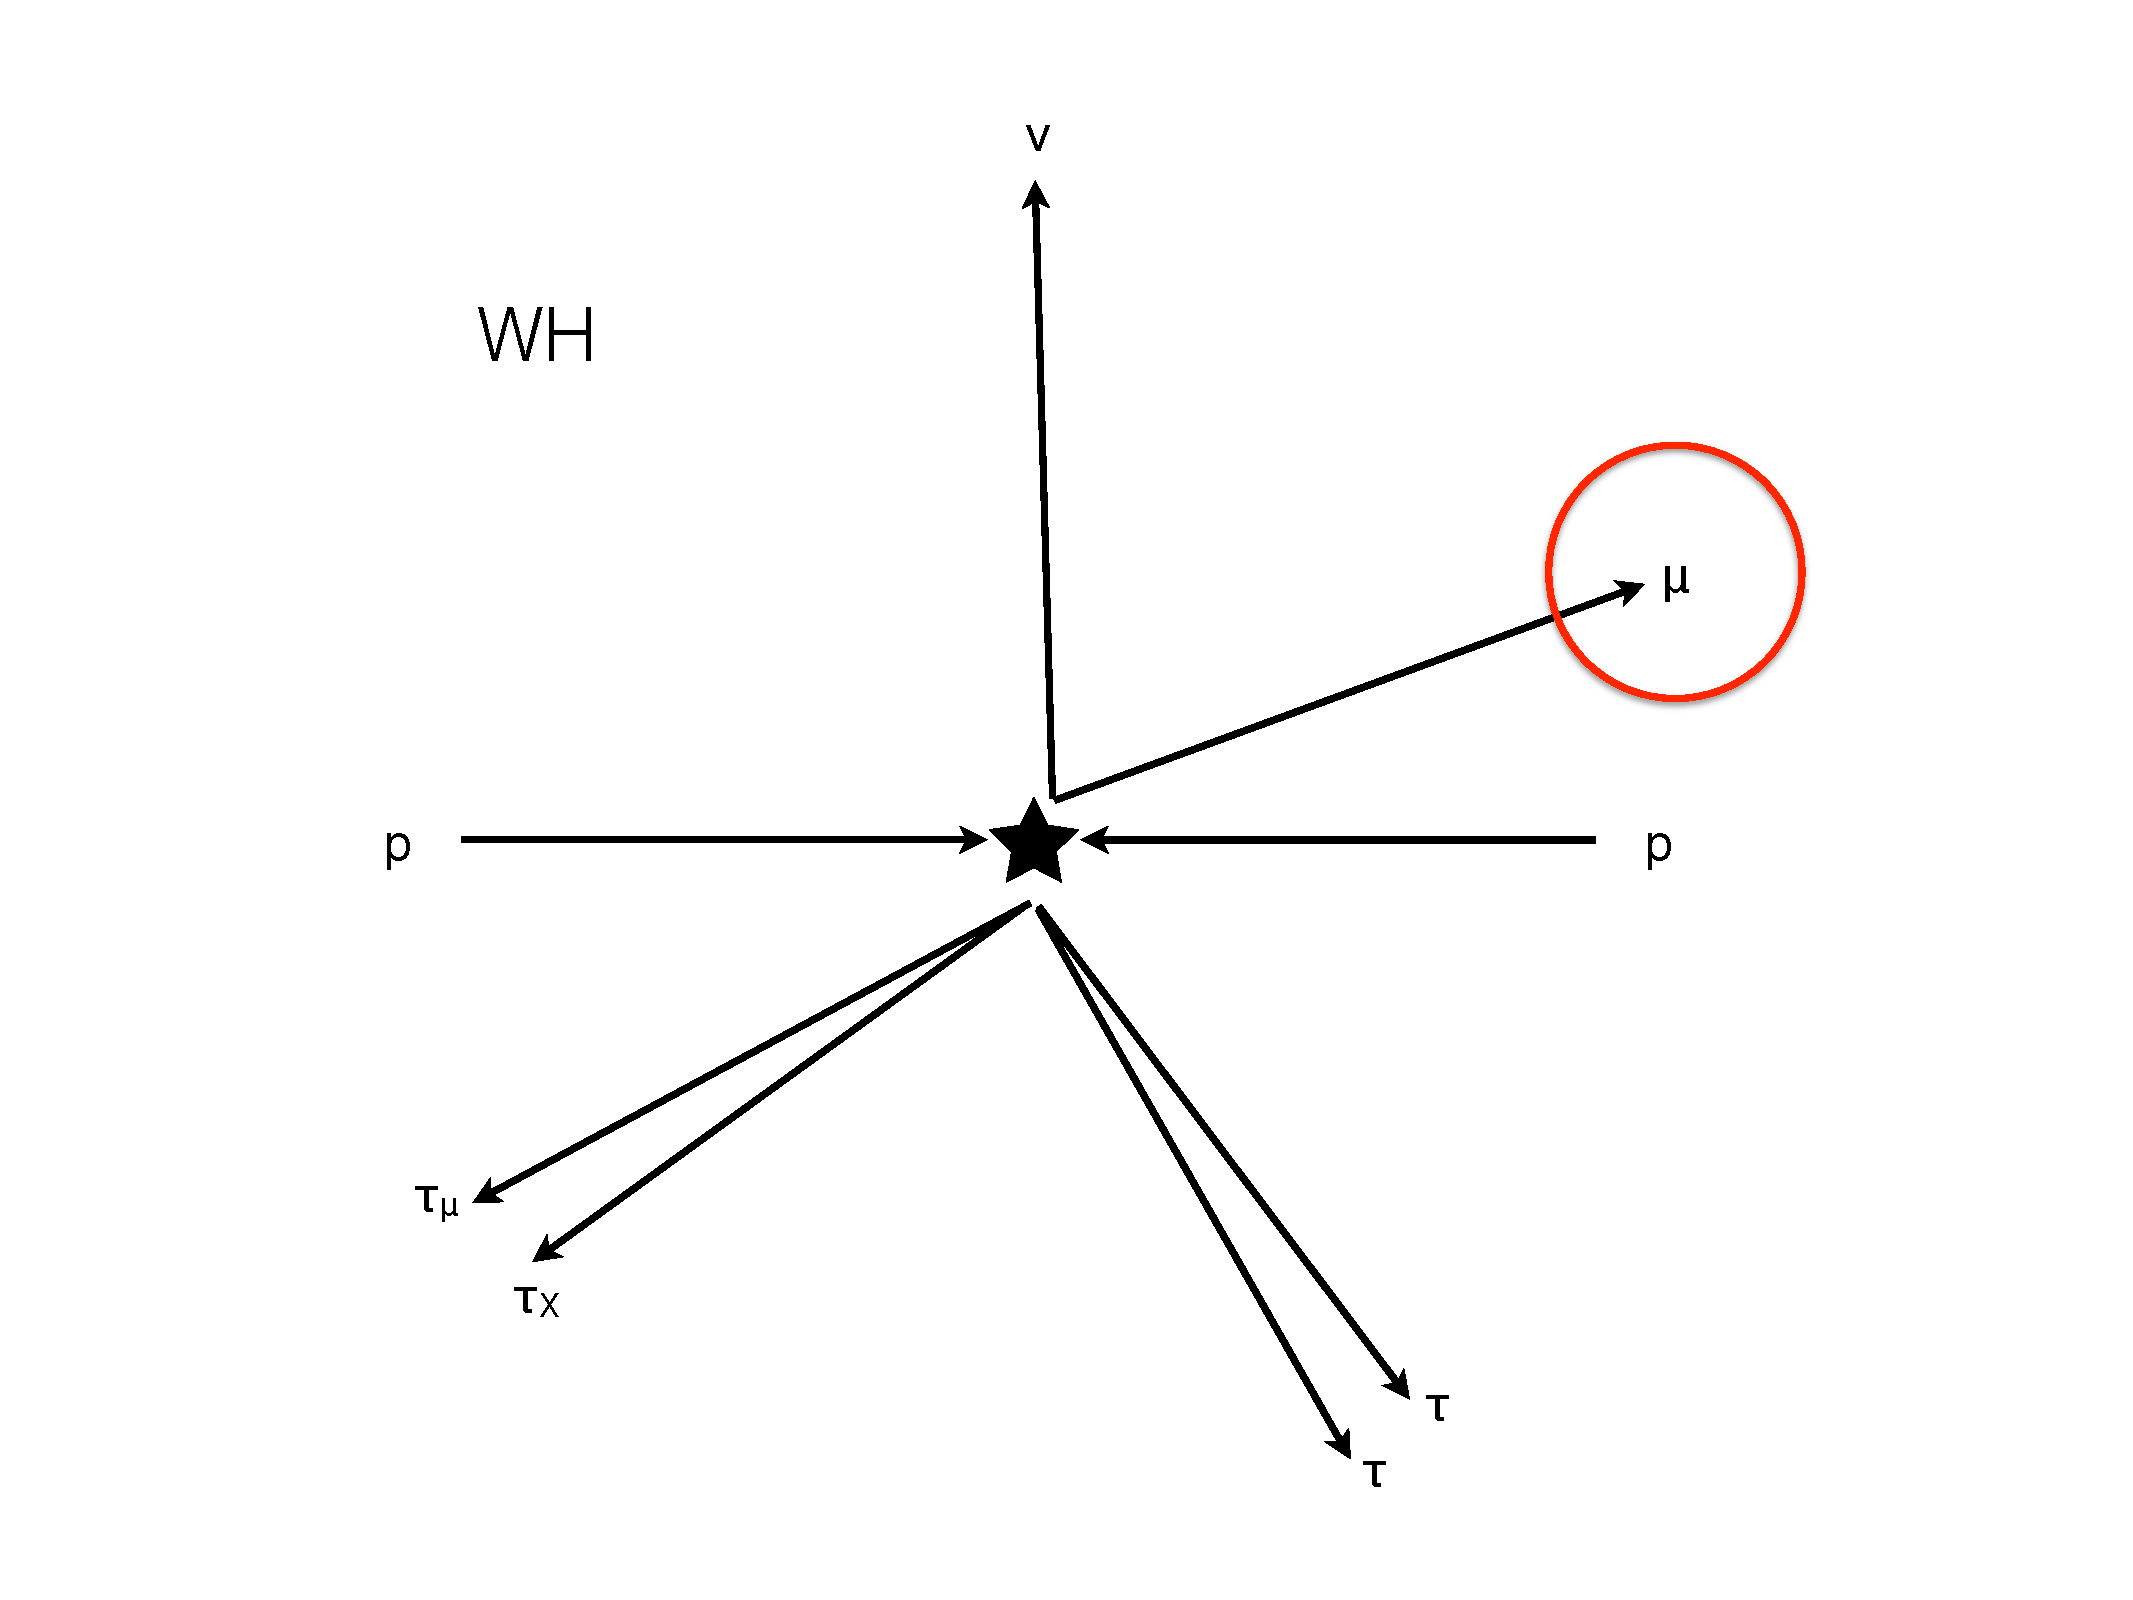
\includegraphics[width=\cmsFigWidth]{figures/WH_trigger}
    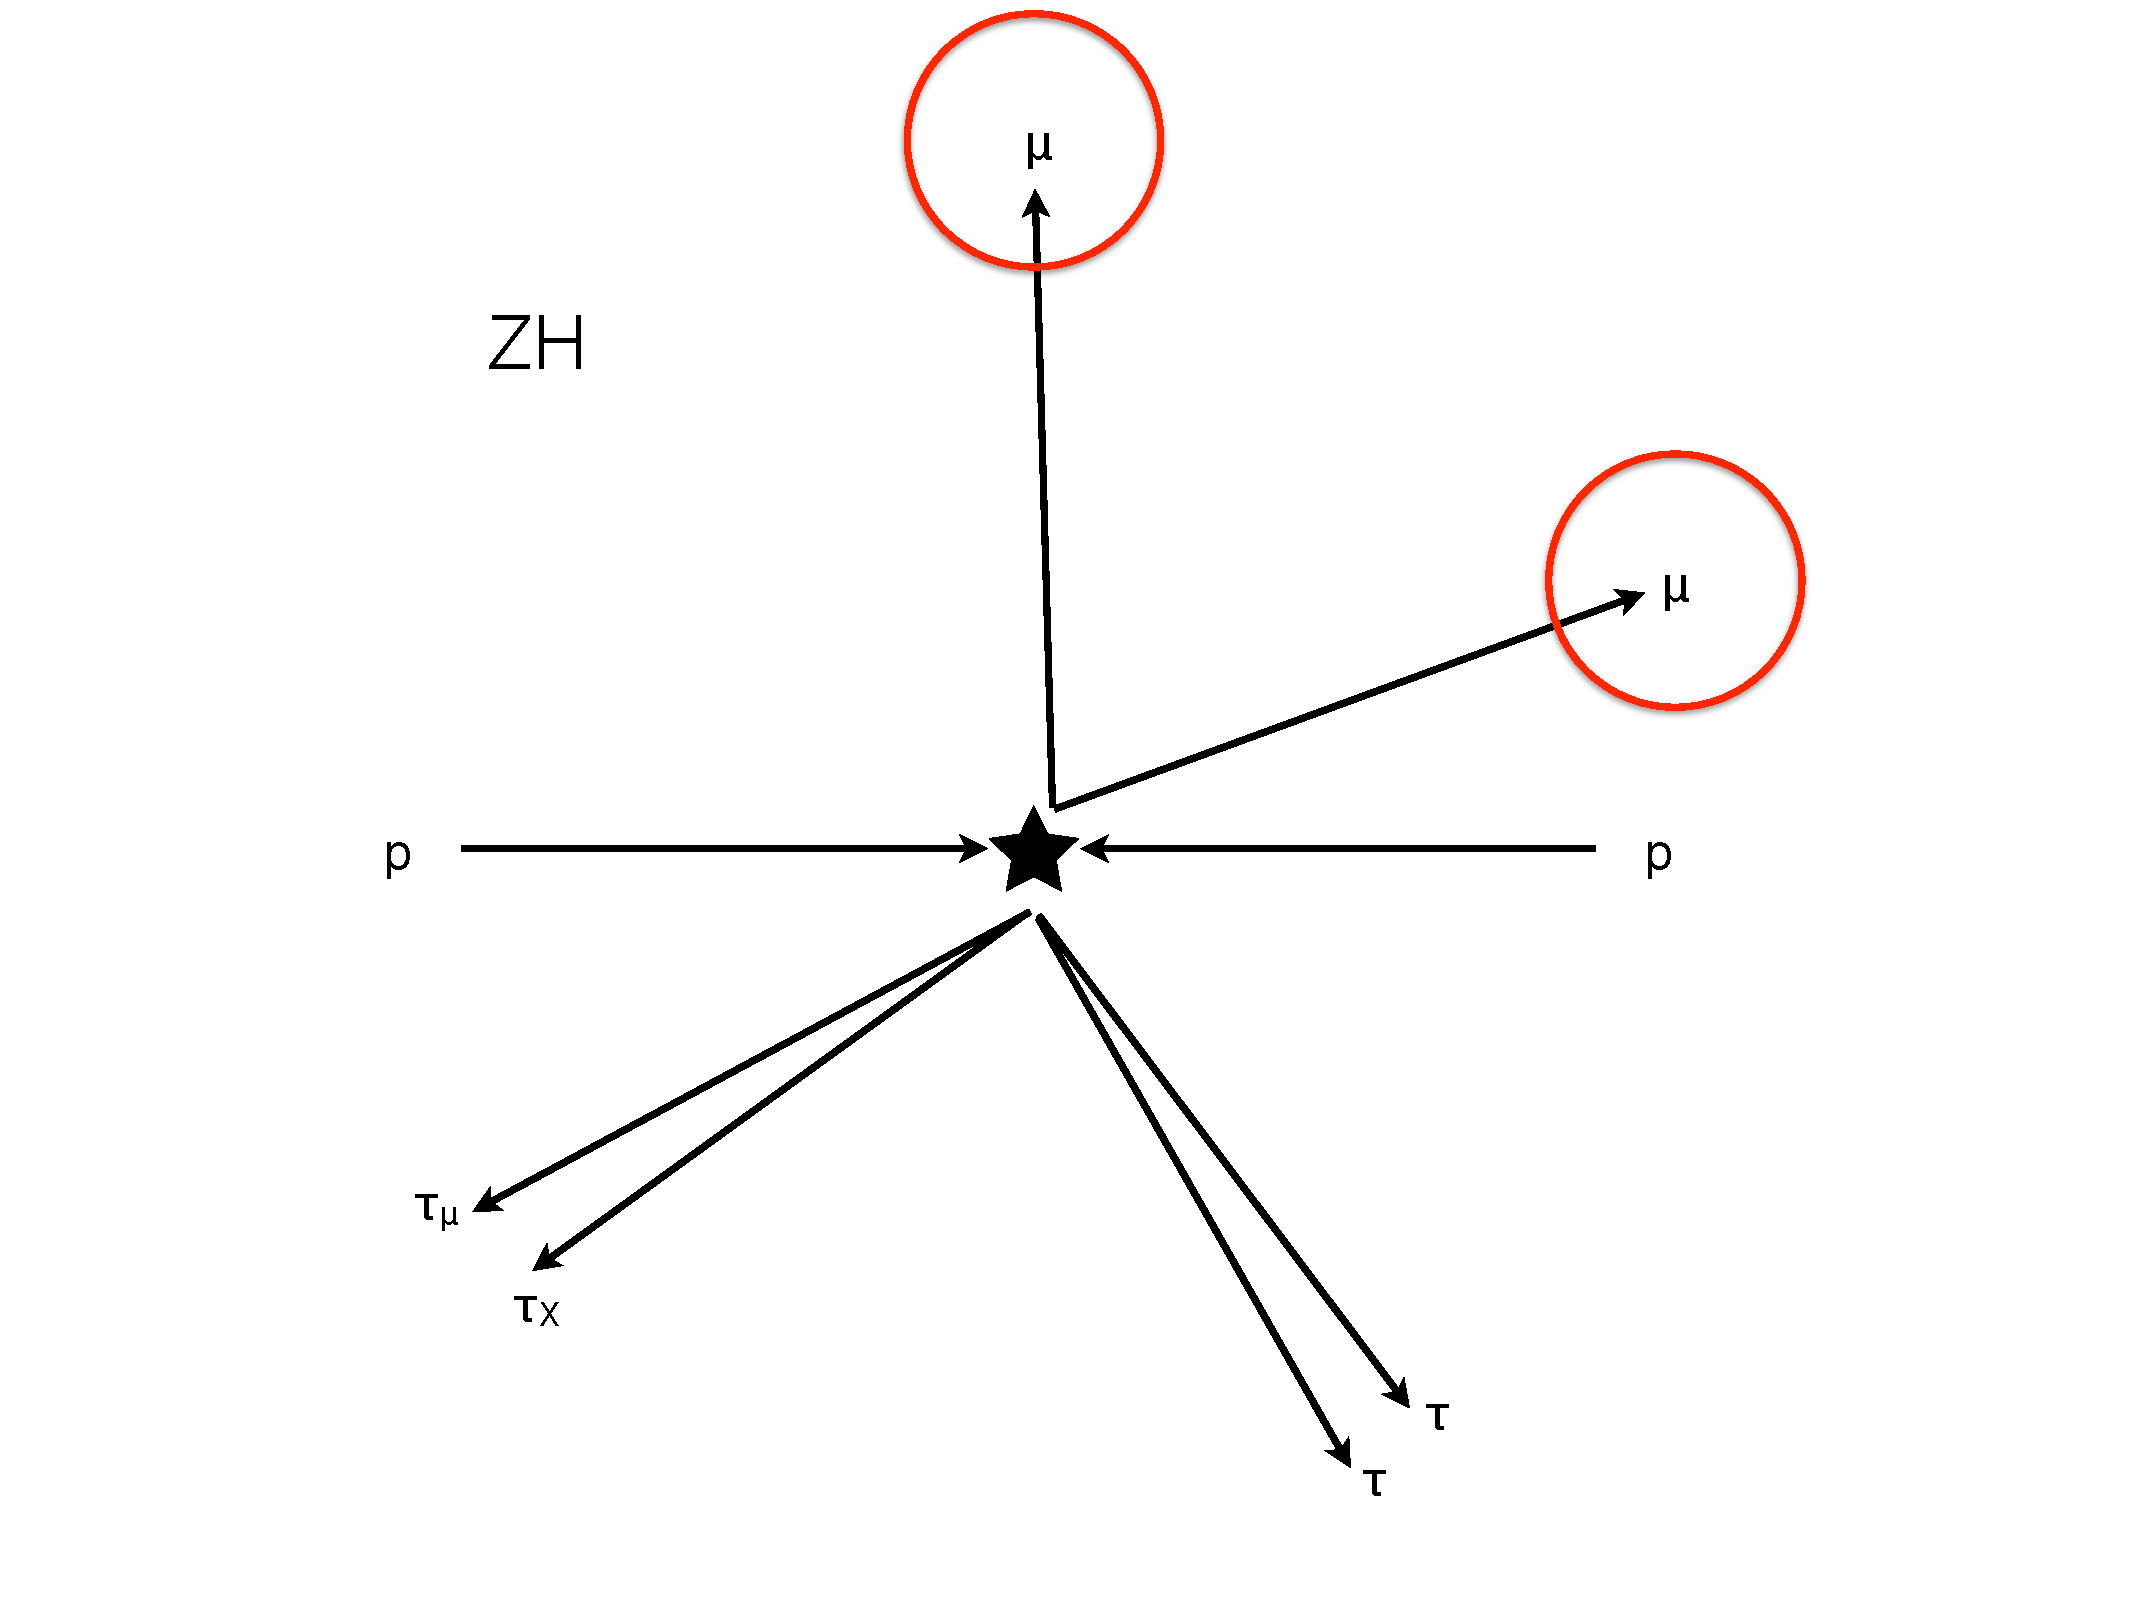
\includegraphics[width=\cmsFigWidth]{figures/ZH_trigger}
    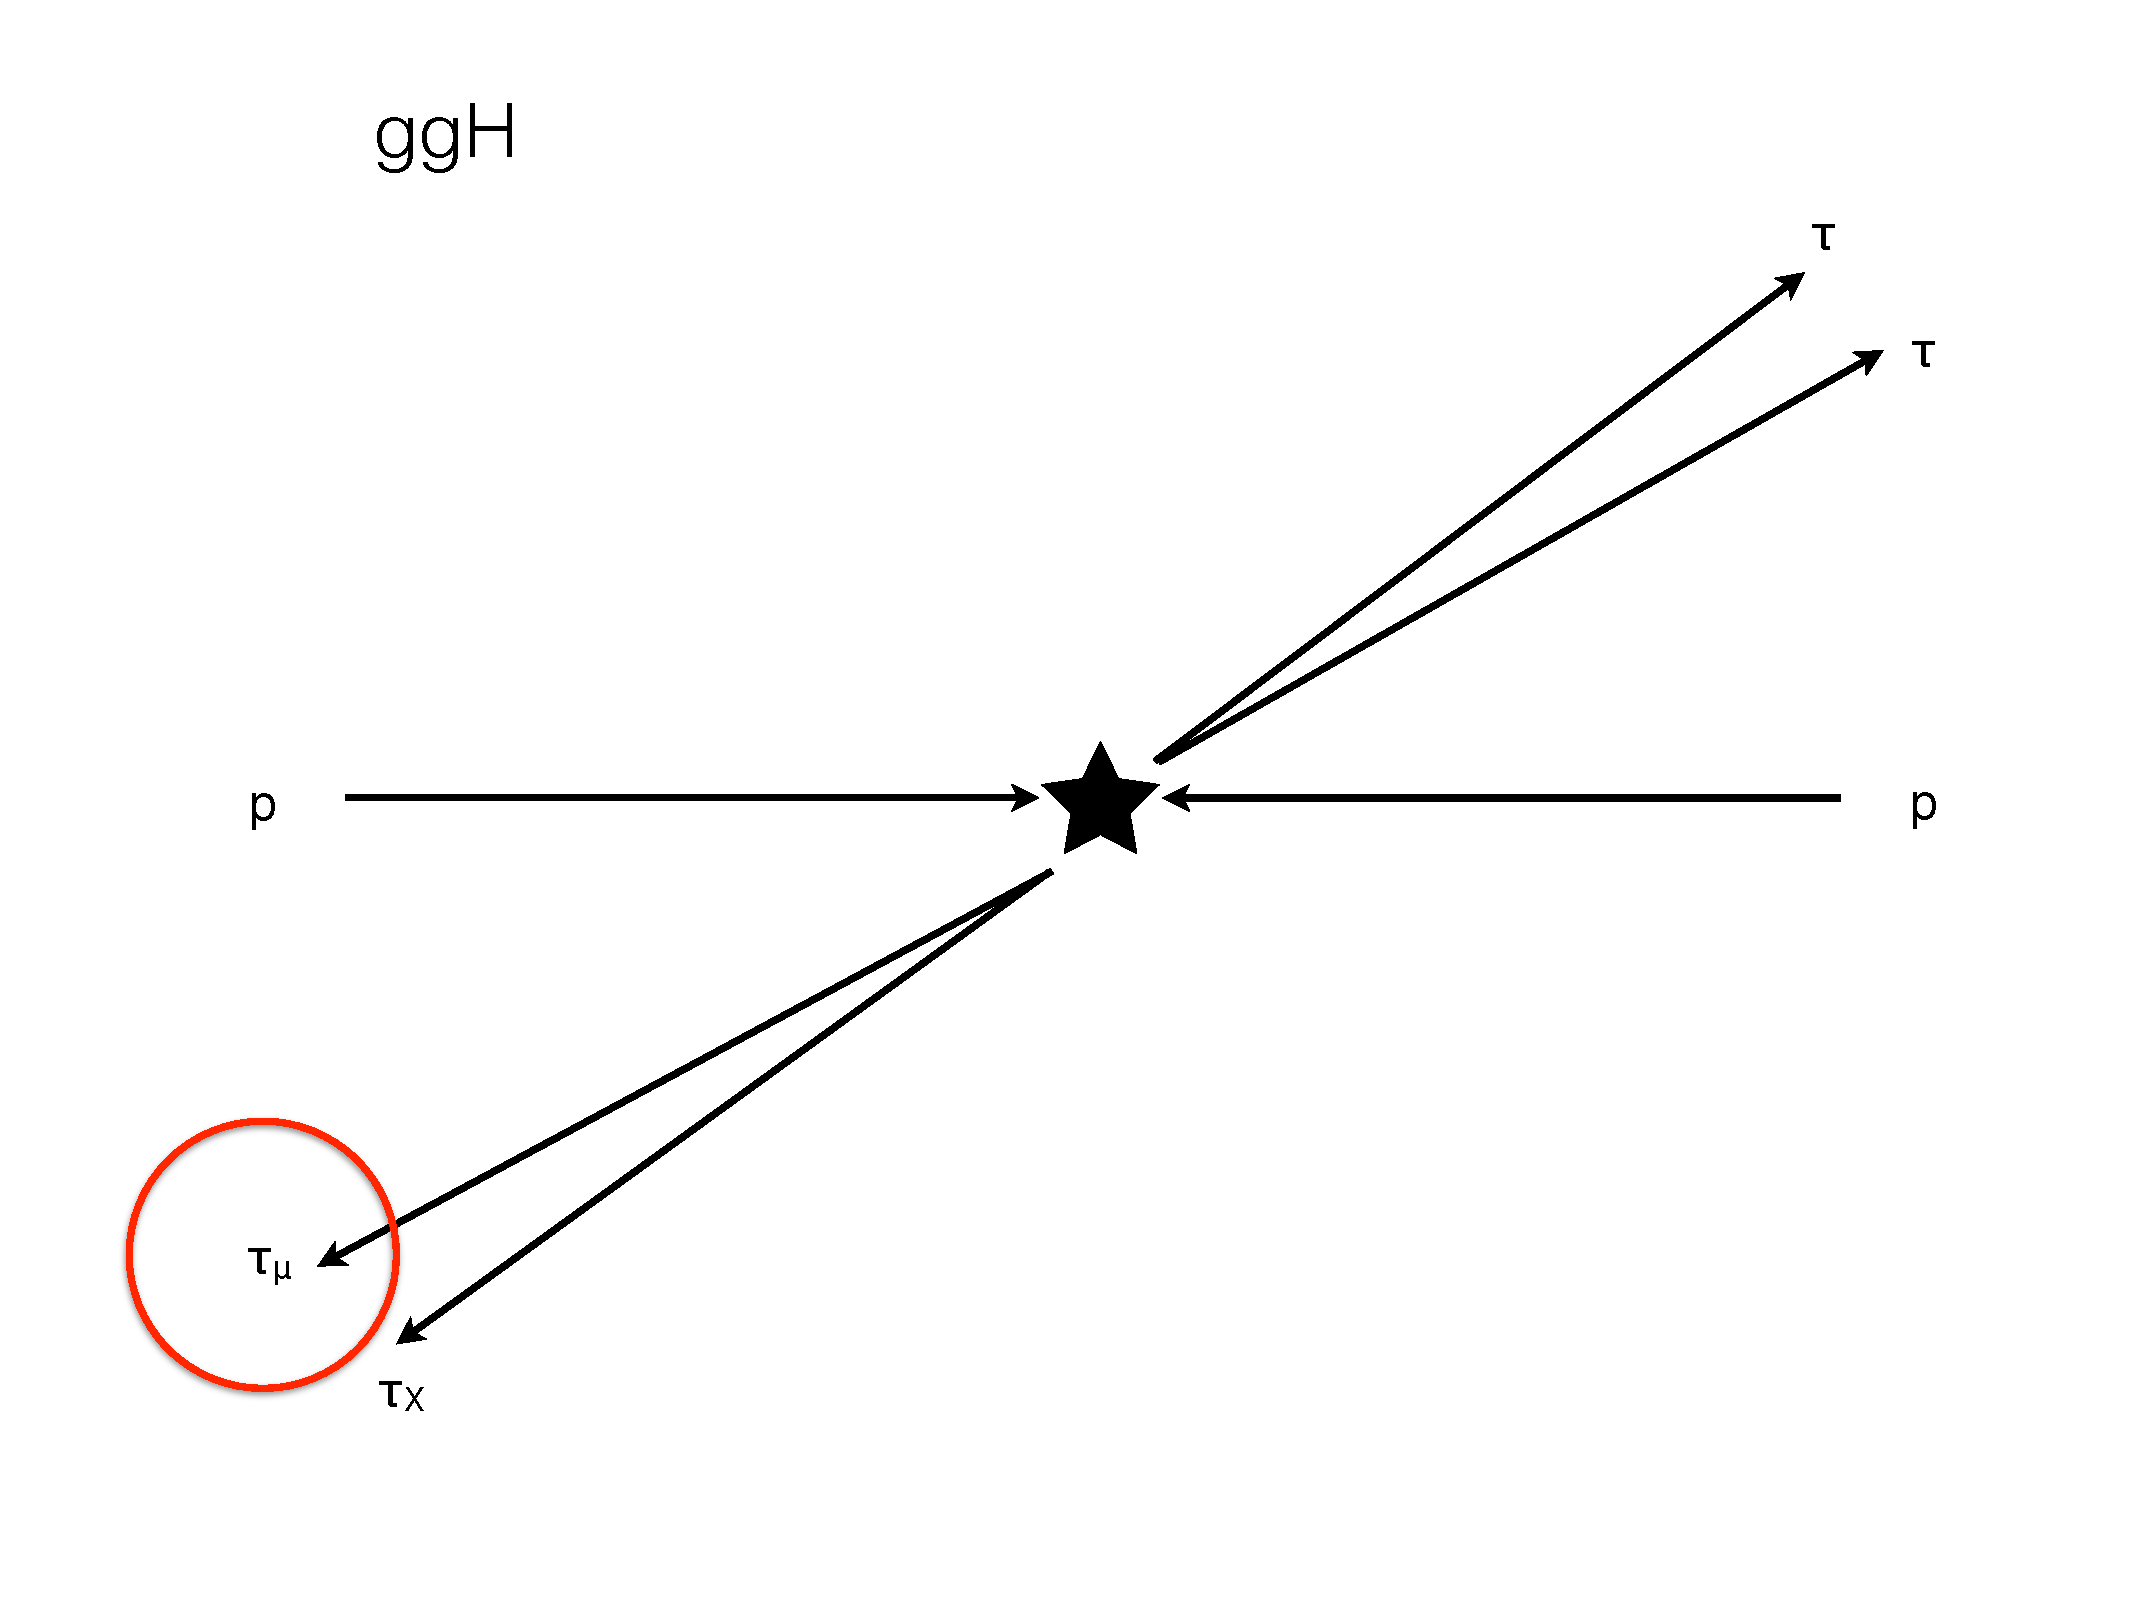
\includegraphics[width=\cmsFigWidth]{figures/ggH_trigger}
    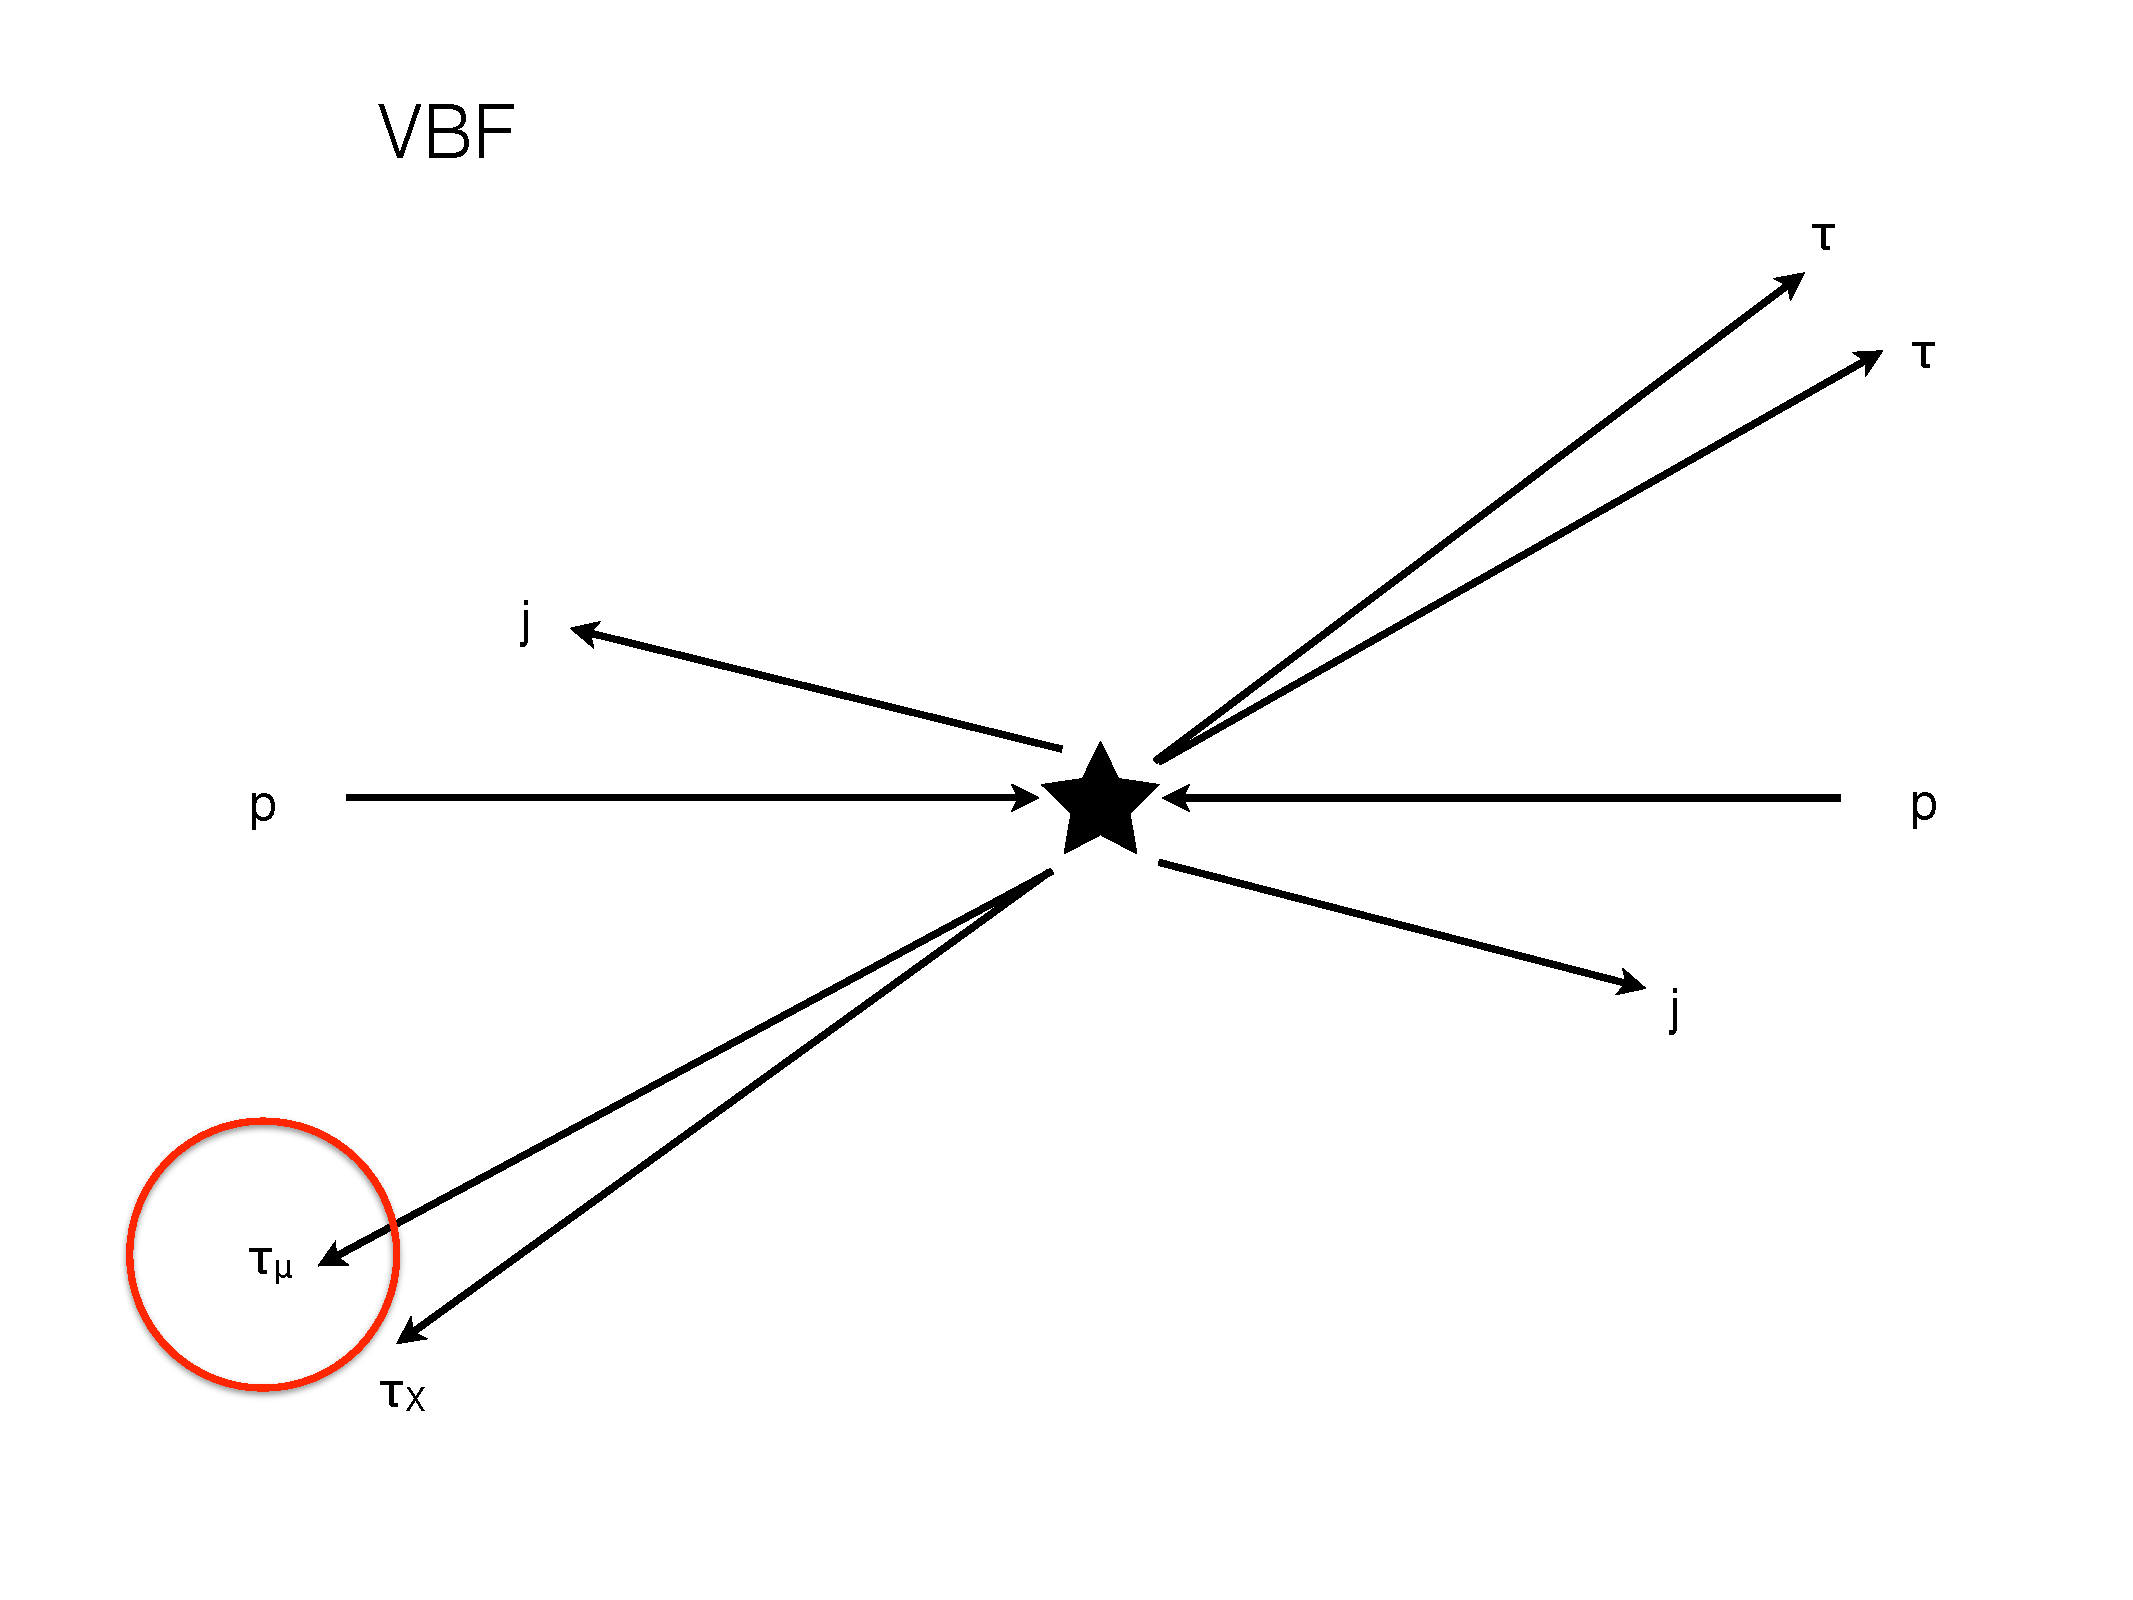
\includegraphics[width=\cmsFigWidth]{figures/VBF_trigger}
    \caption{Diagrams of the four Higgs production modes considered in this search, with the triggering particle circled in red.  (Top \cmsLeft) WH.  (Top \cmsRight) ZH.  (Bottom \cmsLeft) ggH.  (Bottom \cmsRight) VBF.}
    \label{fig:WHZH-vs-ggHVBF-trigger}
  \end{center}
\end{figure}

Due to the boost and low $p_T$ of the pseudoscalar tau decay pairs in ggH and VBF events, most are rejected by \texttt{HLT\_IsoMu24\_eta2p1}.  Those that are accepted fall into two categories:

\begin{enumerate}
\item $a\rightarrow\tau\tau$, one tau decays to a 24 GeV muon and the other tau decays to particles with $p_T$ low enough to pass the HLT muon isolation cut
\item $a\rightarrow\tau\tau$, one tau decays to a 24 GeV muon and the other tau decays far enough away to not be counted in the HLT muon isolation sum
\end{enumerate}

To avoid likely systematic effects in the MC description of ggH and VBF trigger and PF relative isolation efficiency due to the presence of low $p_T$ particles around the trigger muon, events in category 1 are rejected by the nearby lepton isolation requirement.  With this requirement, tau decay muons from the accepted category 2 events appear very similar to muons from $Z$'s or $W$'s, for which \texttt{HLT\_IsoMu24\_eta2p1} and PF relative isolation $<$ 0.12 efficiency measurements and standard scale factors for data-simulation differences are well understood.  The following sections demonstrate that once the nearby lepton isolation requirement is imposed, the efficiency of \texttt{HLT\_IsoMu24\_eta2p1} and PF relative isolation $<$ 0.12 for ggH and VBF tau decay muons in MC is very similar to that of $W$ decay muons in MC.

%HLT efficiency subsection

\subsection{Study of the HLT efficiency for signal events produced via gluon fusion\label{sec:lep-id-eff-ggH-HLT}}
The efficiency for ggH $a\rightarrow\tau\rightarrow\mu$ decay muons to fire \texttt{HLT\_IsoMu24\_eta2p1} is calculated for two reconstructed muon selections.  The first selection is  criteria described in Sec.~\ref{sec:evtsel-triggermu}, except that the nearby lepton isolation requirement is removed.  The second selection is identical to the criteria described in Sec.~\ref{sec:evtsel-triggermu}.  Trigger efficiency is compared for the two selections.  Since the signature of pseudoscalar decays in the detector is similar between the ggH and VBF production modes, the results obtained for ggH simulation can be applied to VBF simulation as well.

The trigger efficiencies of the two selections are given by 

\begin{equation}
\epsilon_{\text{HLT}}^{\text{no }l\text{ iso}} = \frac{\text{No. gen-matched reco'd muons passing no-lepton-isolation ID and HLT}}{\text{No. gen-matched reco'd muons passing trigger muon ID}} \\
\label{eq:muonHLTeff-noliso}
\end{equation}

\begin{equation}
\epsilon_{\text{HLT}} = \frac{\text{No. gen-matched reco'd muons passing trigger muon ID and HLT}}{\text{No. gen-matched reco'd muons passing trigger muon ID}} \\
\label{eq:muonHLTeff}
\end{equation}

where

\begin{itemize}
\item the gen-matching criteria is $\Delta$$p_T$(reco muon, gen $a\rightarrow\tau\rightarrow\mu$ muon) $<$ 0.1 GeV and the gen muon is from the decay of a tau that is itself from the decay of a pseudoscalar;
\item the trigger muon ID for $\epsilon_{\text{HLT}}^{\text{no }l\text{ iso}}$ is as described in Sec.~\ref{sec:evtsel-triggermu} but with the nearby lepton isolation requirement removed;
\item the trigger muon ID for $\epsilon_{\text{HLT}}$ is as described in Sec.~\ref{sec:evtsel-triggermu}; and
\item ``HLT'' refers to firing \texttt{HLT\_IsoMu24\_eta2p1}.
\end{itemize}

Figure~\ref{fig:HLTEffVsDR} shows $\epsilon_{\text{HLT}}^{\text{no }l\text{ iso}}$ as a function of $\Delta$R(gen $a\rightarrow\tau\rightarrow\mu$ muon, gen $\tau_{\text{2}}$), where the gen $a\rightarrow\tau\rightarrow\mu$ muon is matched to the reco'd muon as described in Eq.~\ref{eq:muonHLTeff-noliso} above and the gen $\tau_{\text{2}}$ is the other tau from the $a\rightarrow\tau\tau$ decay.  The efficiency is calculated separately for each decay mode of the gen $\tau_{\text{2}}$ (electronic, muonic, or hadronic).  $\epsilon_{\text{HLT}}^{\text{no }l\text{ iso}}$ is $\sim$90\% for $\Delta$R $>$ 0.4, when the two taus from pseudoscalar decay are separated enough that the tau decay muon appears isolated. This is similar to the efficiency of \texttt{HLT\_IsoMu24\_eta2p1} for $W$ decay muons~\cite{1748-0221-7-10-P10002}.  When the two taus are closer than $\Delta$R $\sim$ 0.4, the efficiency decreases because the non-triggering tau spoils the isolation of the tau decay muon that fires the trigger.  The effect is worst in the $\tau_{\mu}\tau_{e}$ and $\tau_{\mu}\tau_{\mu}$ modes because electrons and muons contribute to isolation at the trigger level, but are not counted in the offline PF relative isolation.

\begin{figure}[hbtp]
  \begin{center}
    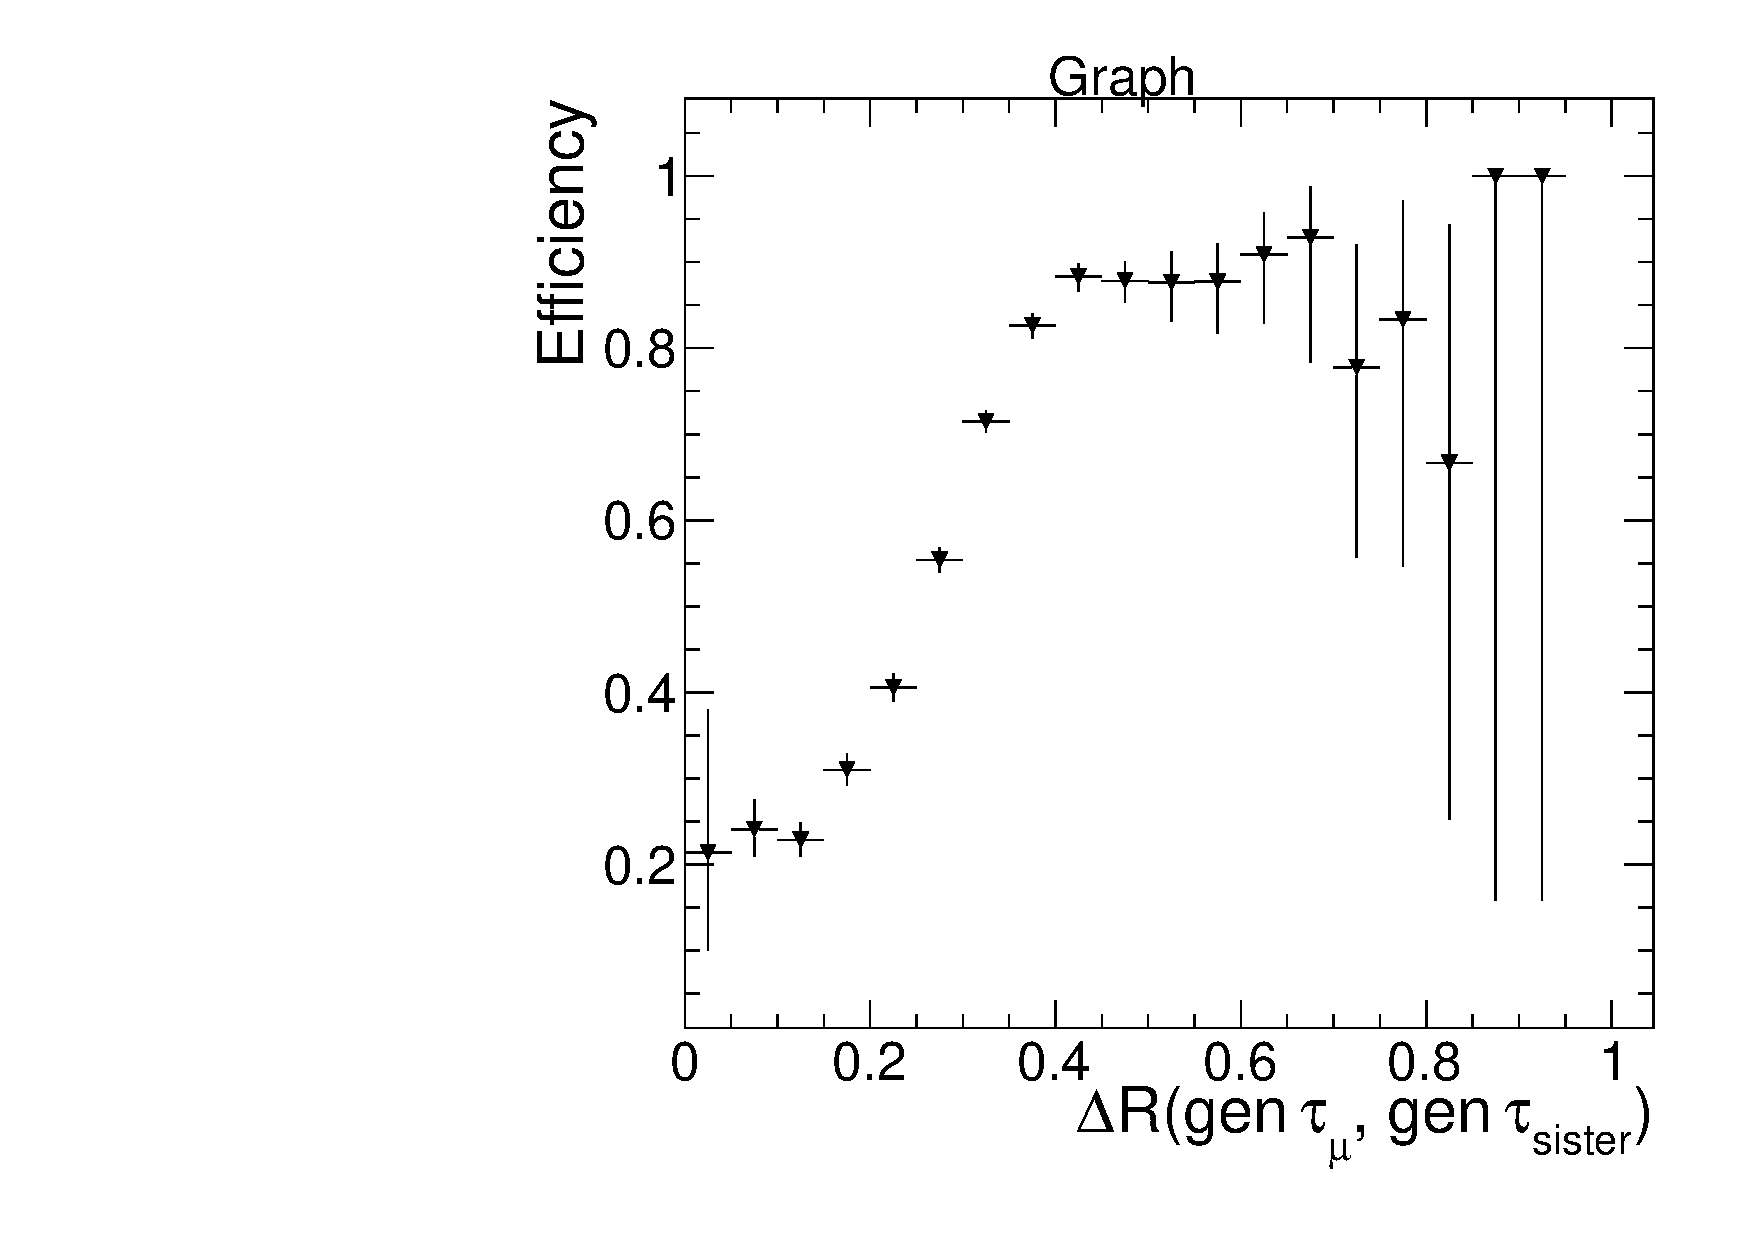
\includegraphics[width=0.8\cmsFigWidth]{figures/dREfficiency_WmuIDIso_muEOnly}
    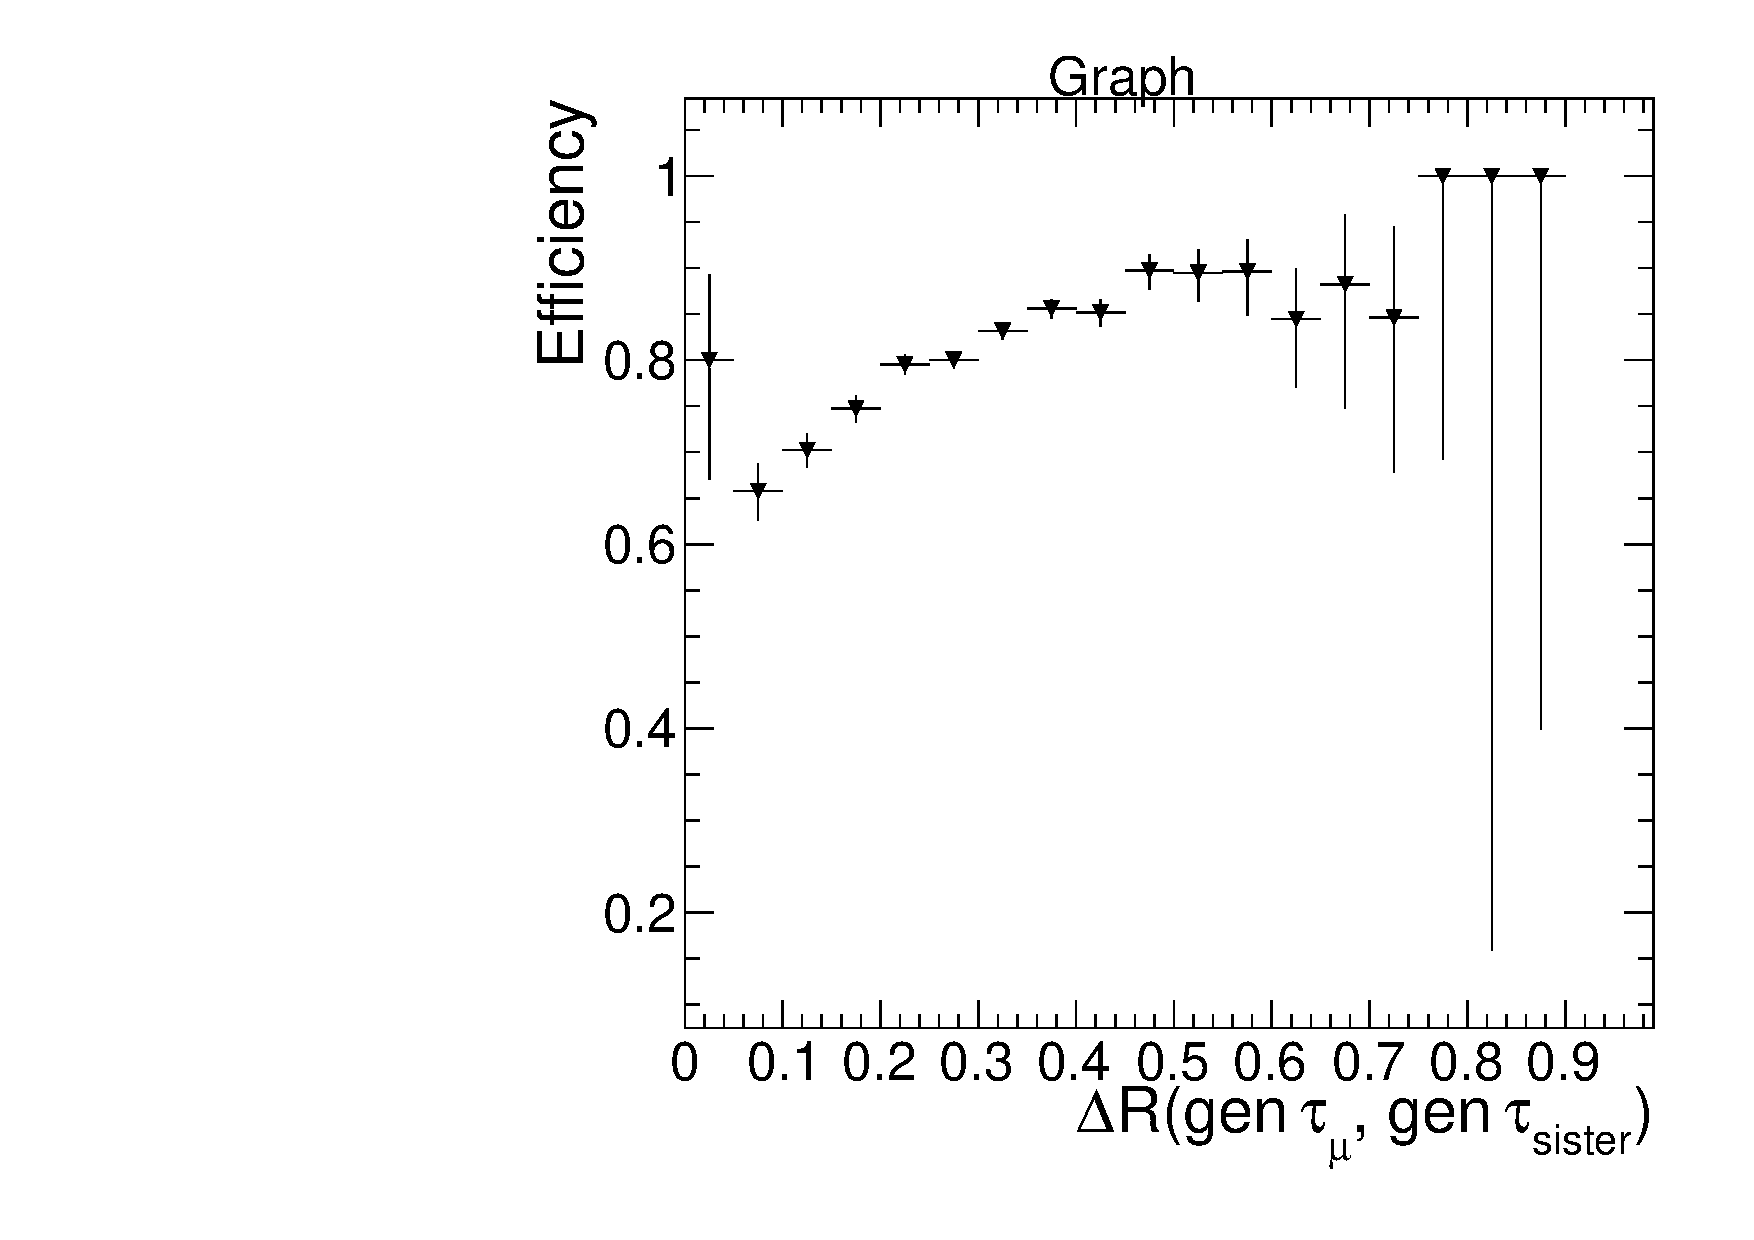
\includegraphics[width=0.8\cmsFigWidth]{figures/dREfficiency_WmuIDIso_muMuOnly}
    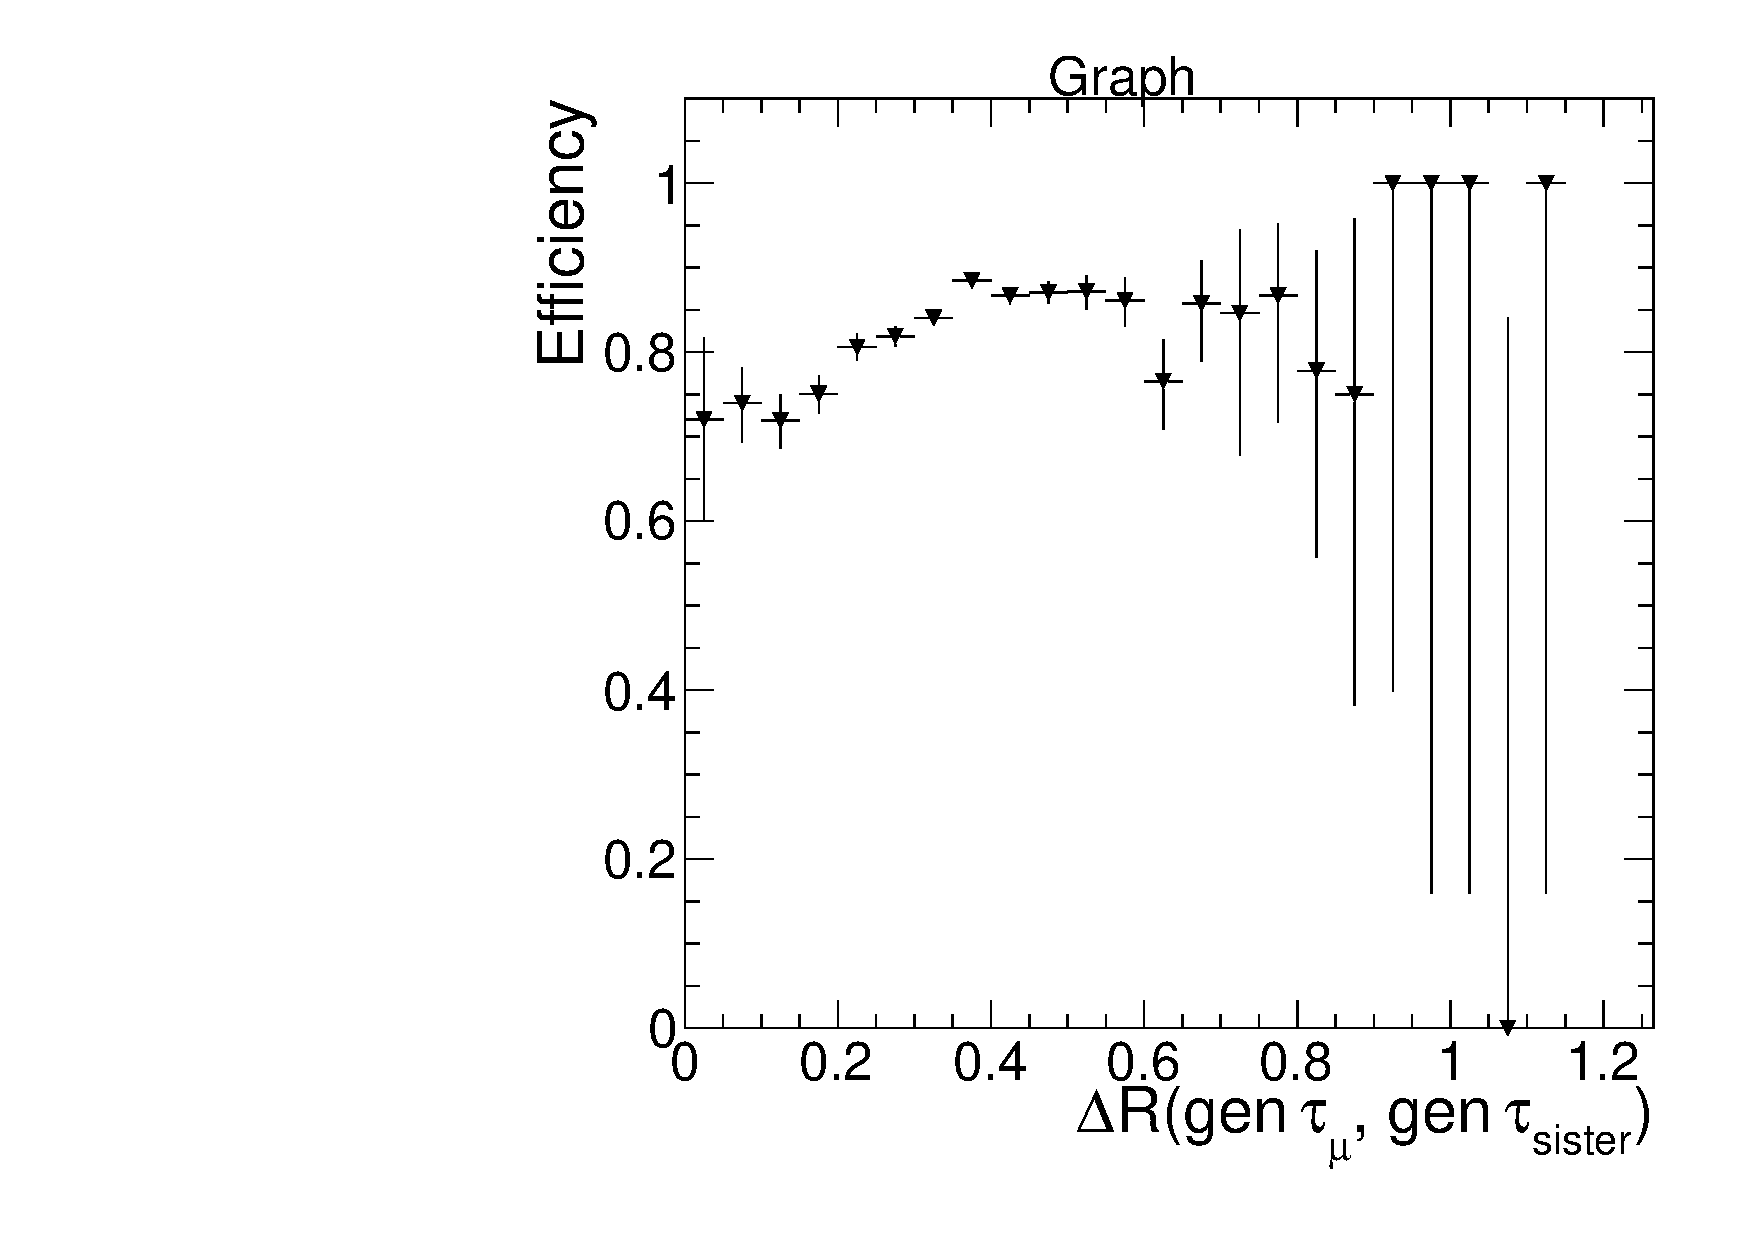
\includegraphics[width=0.8\cmsFigWidth]{figures/dREfficiency_WmuIDIso_muHadOnly}
    \caption{$\epsilon_{\text{HLT}}^{\text{no }l\text{ iso}}$ for the ggH signal as a function of the separation $\Delta$R(gen $a\rightarrow\tau\rightarrow\mu$ muon, gen $\tau_{\text{2}}$), where the gen $\tau_{\text{2}}$ is a decay product of the same pseudoscalar as in the $a\rightarrow\tau\rightarrow\mu$.  The $a\rightarrow\tau\rightarrow\mu$ muon is matched to the reco'd muon as described in the text.  The reco'd muon is required to pass the trigger muon ID of Sec.~\ref{sec:evtsel-triggermu}, but with the nearby lepton isolation requirement removed.  (\cmsLeft) Gen $\tau_{\text{2}}$ decays to an electron.  (middle) Gen $\tau_{\text{2}}$ decays to a muon.  (\cmsRight) Gen $\tau_{\text{2}}$ decays to hadrons.}
    \label{fig:HLTEffVsDR}
  \end{center}
\end{figure}

In contrast, Figure~\ref{fig:HLTEffVsDR_withFilters} shows $\epsilon_{\text{HLT}}$ as a function of $\Delta$R(gen $a\rightarrow\tau\rightarrow\mu$ muon, gen $\tau_{\text{2}}$), where the gen $a\rightarrow\tau\rightarrow\mu$ muon is matched to the reco'd muon as described in Eq.~\ref{eq:muonHLTeff} above and the gen $\tau_{\text{2}}$ is the other tau from the $a\rightarrow\tau\rightarrow\mu$ decay.  The efficiency is calculated separately for each decay mode of the gen $\tau_{\text{2}}$ (electronic, muonic, or hadronic).  The efficiencies are much flatter in $\Delta$R when the nearby lepton isolation requirement is applied to the reconstructed trigger muon, because it ensures that events can pass the selection sequence only if the two reconstructed taus from the pseudoscalar decay are well separated.  The trigger efficiency for $a\rightarrow\tau\rightarrow\mu$ muons in these events is similar to that of $W$ decay muons and is in the regime where the trigger muon is isolated and MC describes the data well.

\begin{figure}[hbtp]
  \begin{center}
    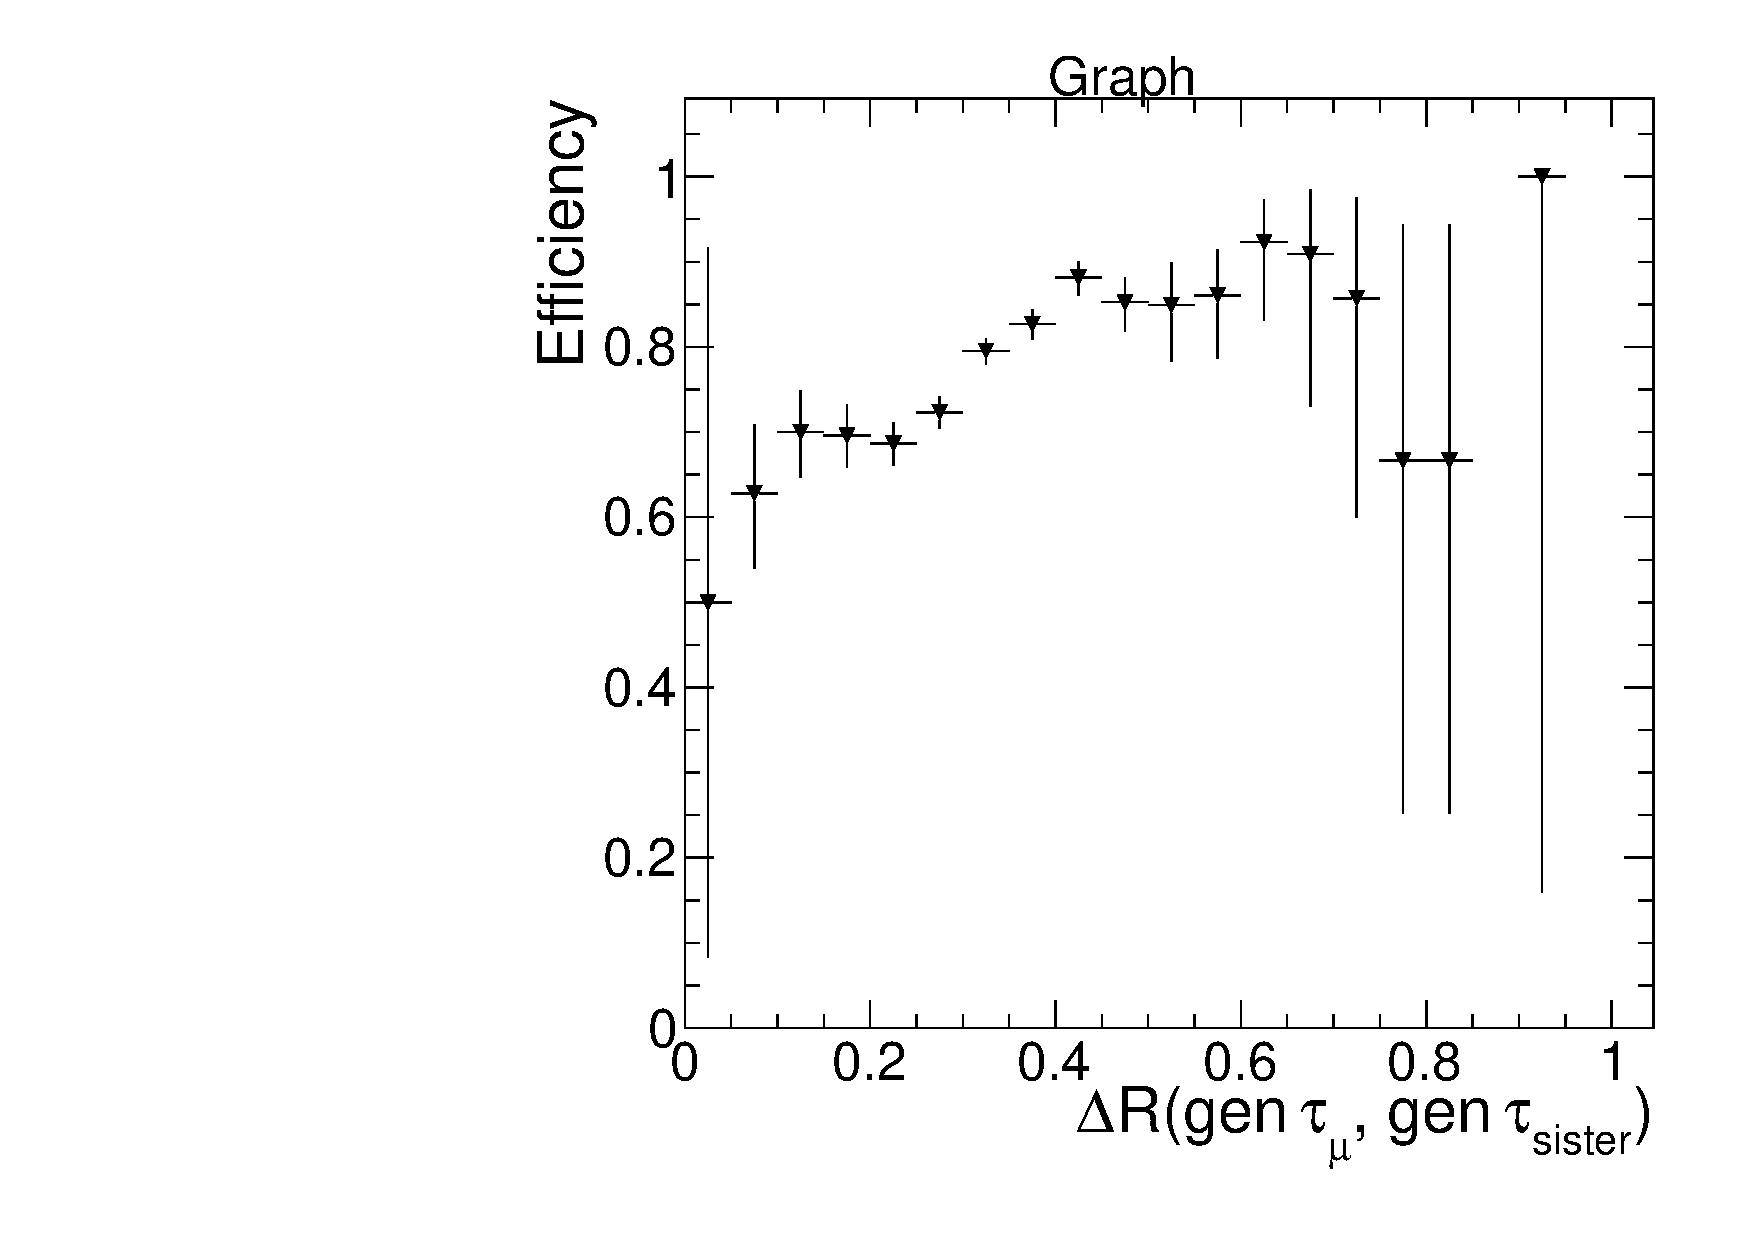
\includegraphics[width=0.8\cmsFigWidth]{figures/dRHLTEfficiency_WmuIDIso_withFilters_muEOnly}
    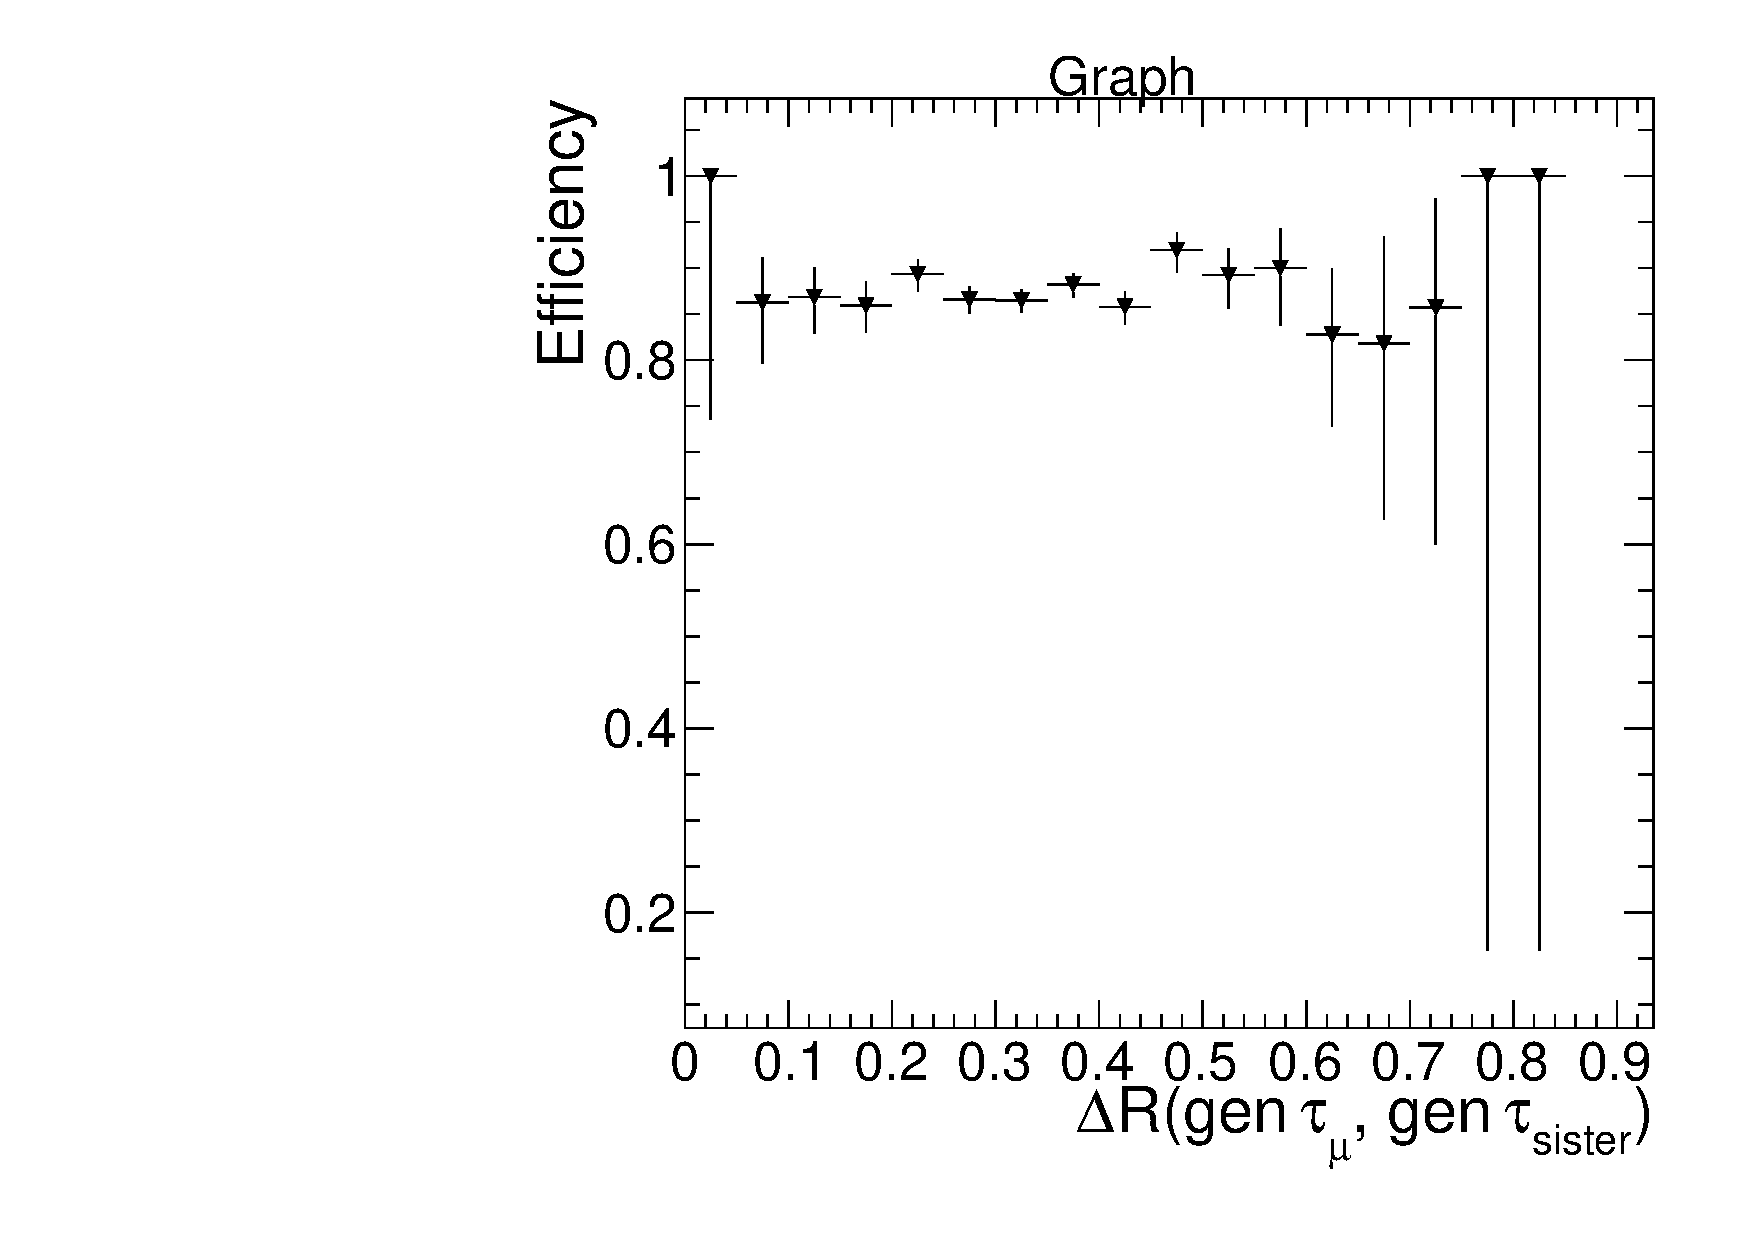
\includegraphics[width=0.8\cmsFigWidth]{figures/dRHLTEfficiency_WmuIDIso_withFilters_muMuOnly}
    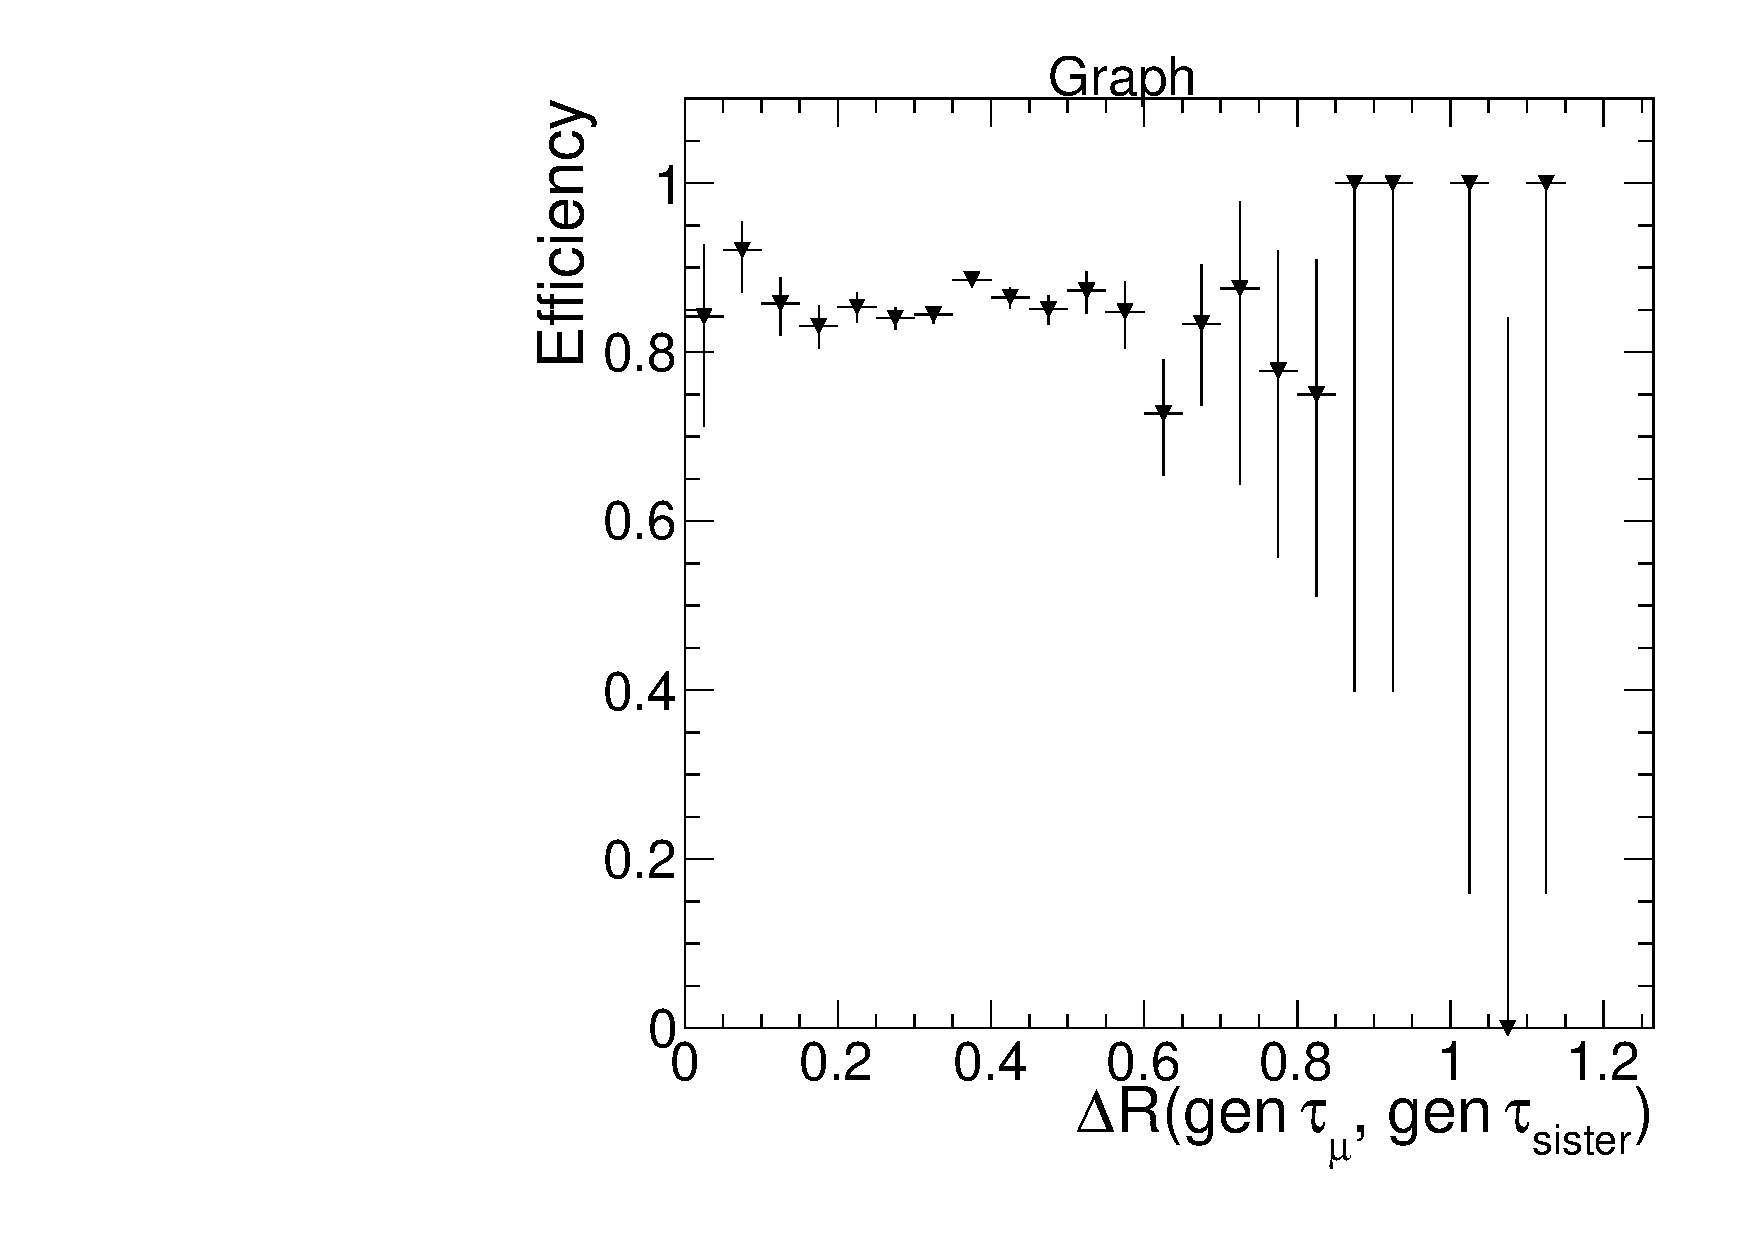
\includegraphics[width=0.8\cmsFigWidth]{figures/dRHLTEfficiency_WmuIDIso_withFilters_muHadOnly}
    \caption{$\epsilon_{\text{HLT}}$ for the ggH signal as a function of the separation $\Delta$R(gen $a\rightarrow\tau\rightarrow\mu$ muon, gen $\tau_{\text{2}}$), where the gen $\tau_{\text{2}}$ is a decay product of the same pseudoscalar as in the $a\rightarrow\tau\rightarrow\mu$.  The $a\rightarrow\tau\rightarrow\mu$ muon is matched to the reco'd muon as described in the text.  The reco'd muon is required to pass the trigger muon ID of Sec.~\ref{sec:evtsel-triggermu}.  (\cmsLeft) Gen $\tau_{\text{2}}$ decays to an electron.  (middle) Gen $\tau_{\text{2}}$ decays to a muon.  (\cmsRight) Gen $\tau_{\text{2}}$ decays to hadrons.}
    \label{fig:HLTEffVsDR_withFilters}
  \end{center}
\end{figure}

Figure~\ref{fig:HLT-eff-W-mu} shows the HLT efficiency for muons passing the trigger muon ID in both the WH and gluon fusion production modes.  In both modes, the trigger muon ID includes the nearby lepton non-overlap requirement.  The efficiencies are very similar for the reasons discussed above.

\begin{figure}[hbtp]
  \begin{center}
    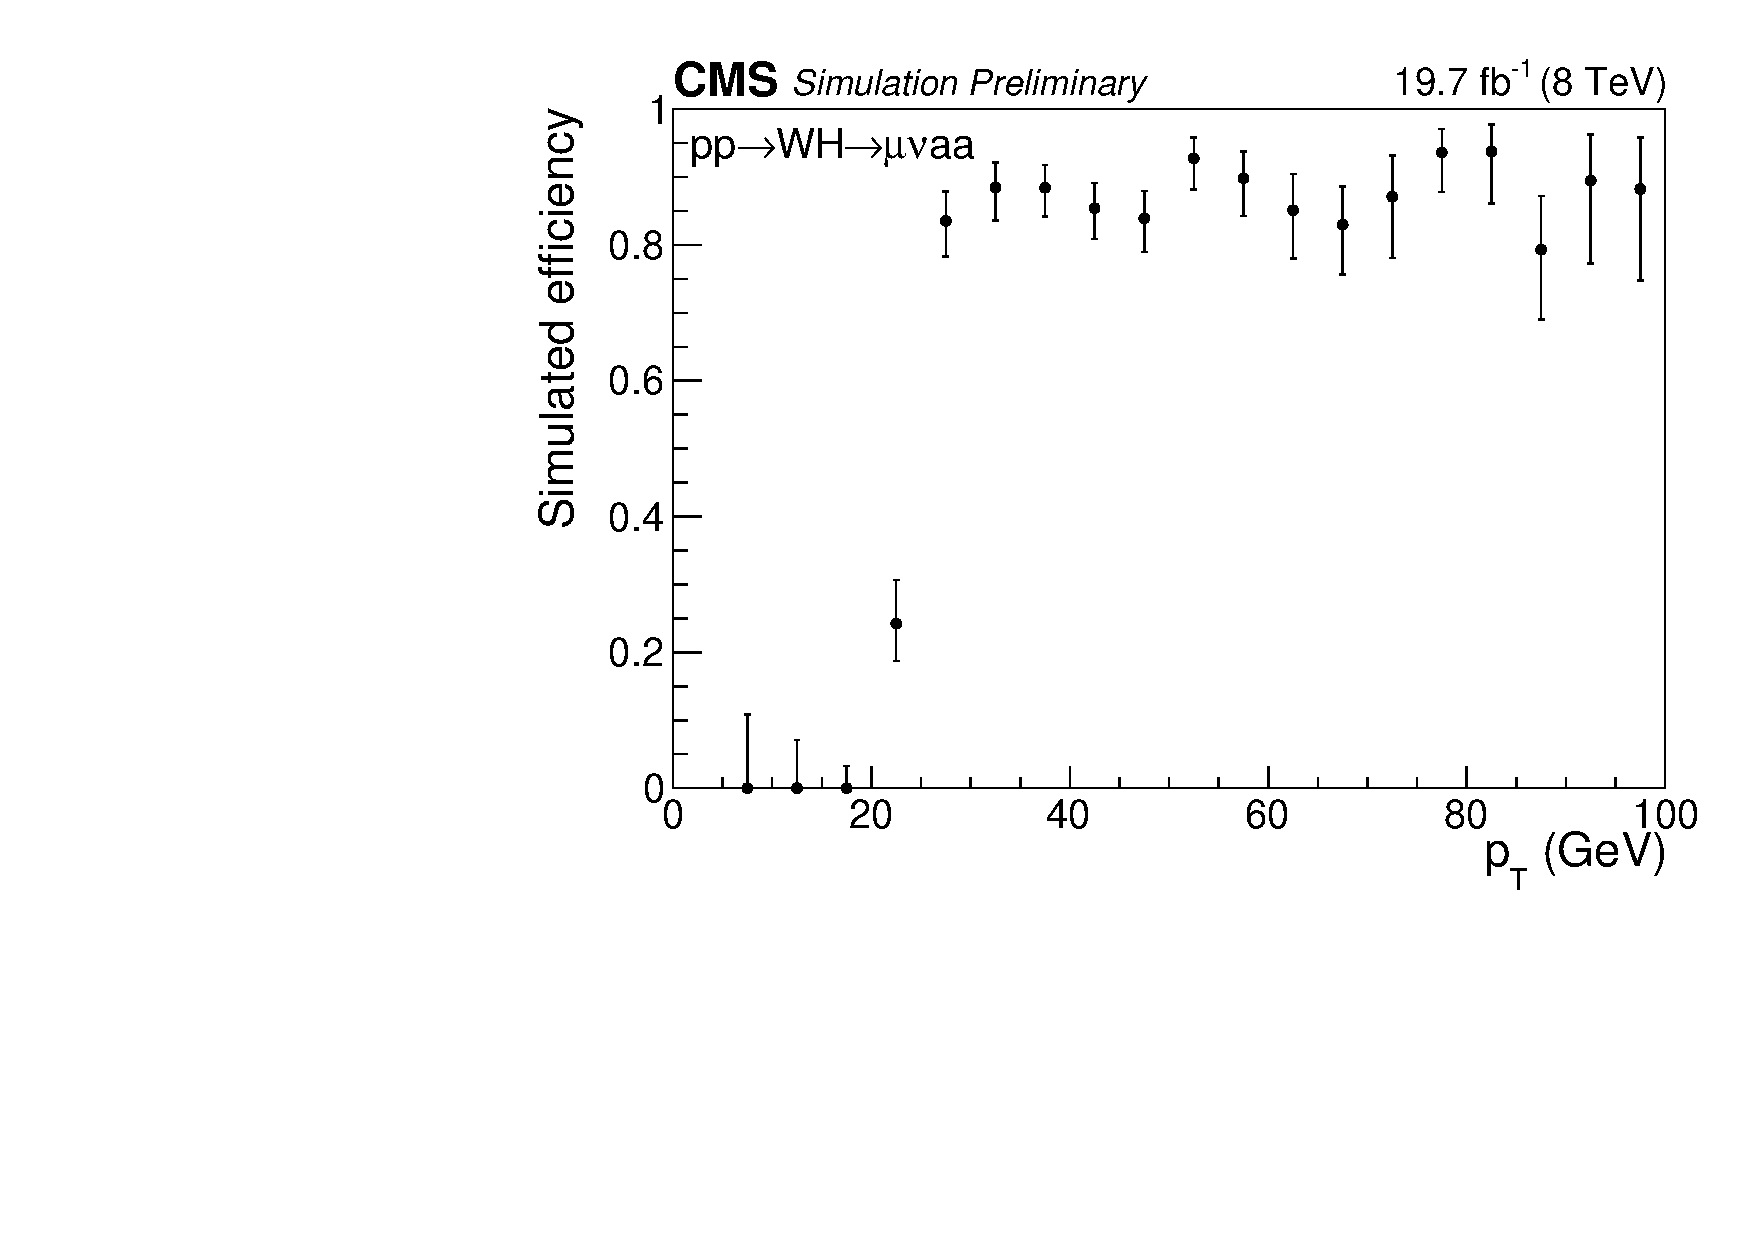
\includegraphics[width=1.24\cmsFigWidth]{figures/HLT_eff_Wmu_WH}
    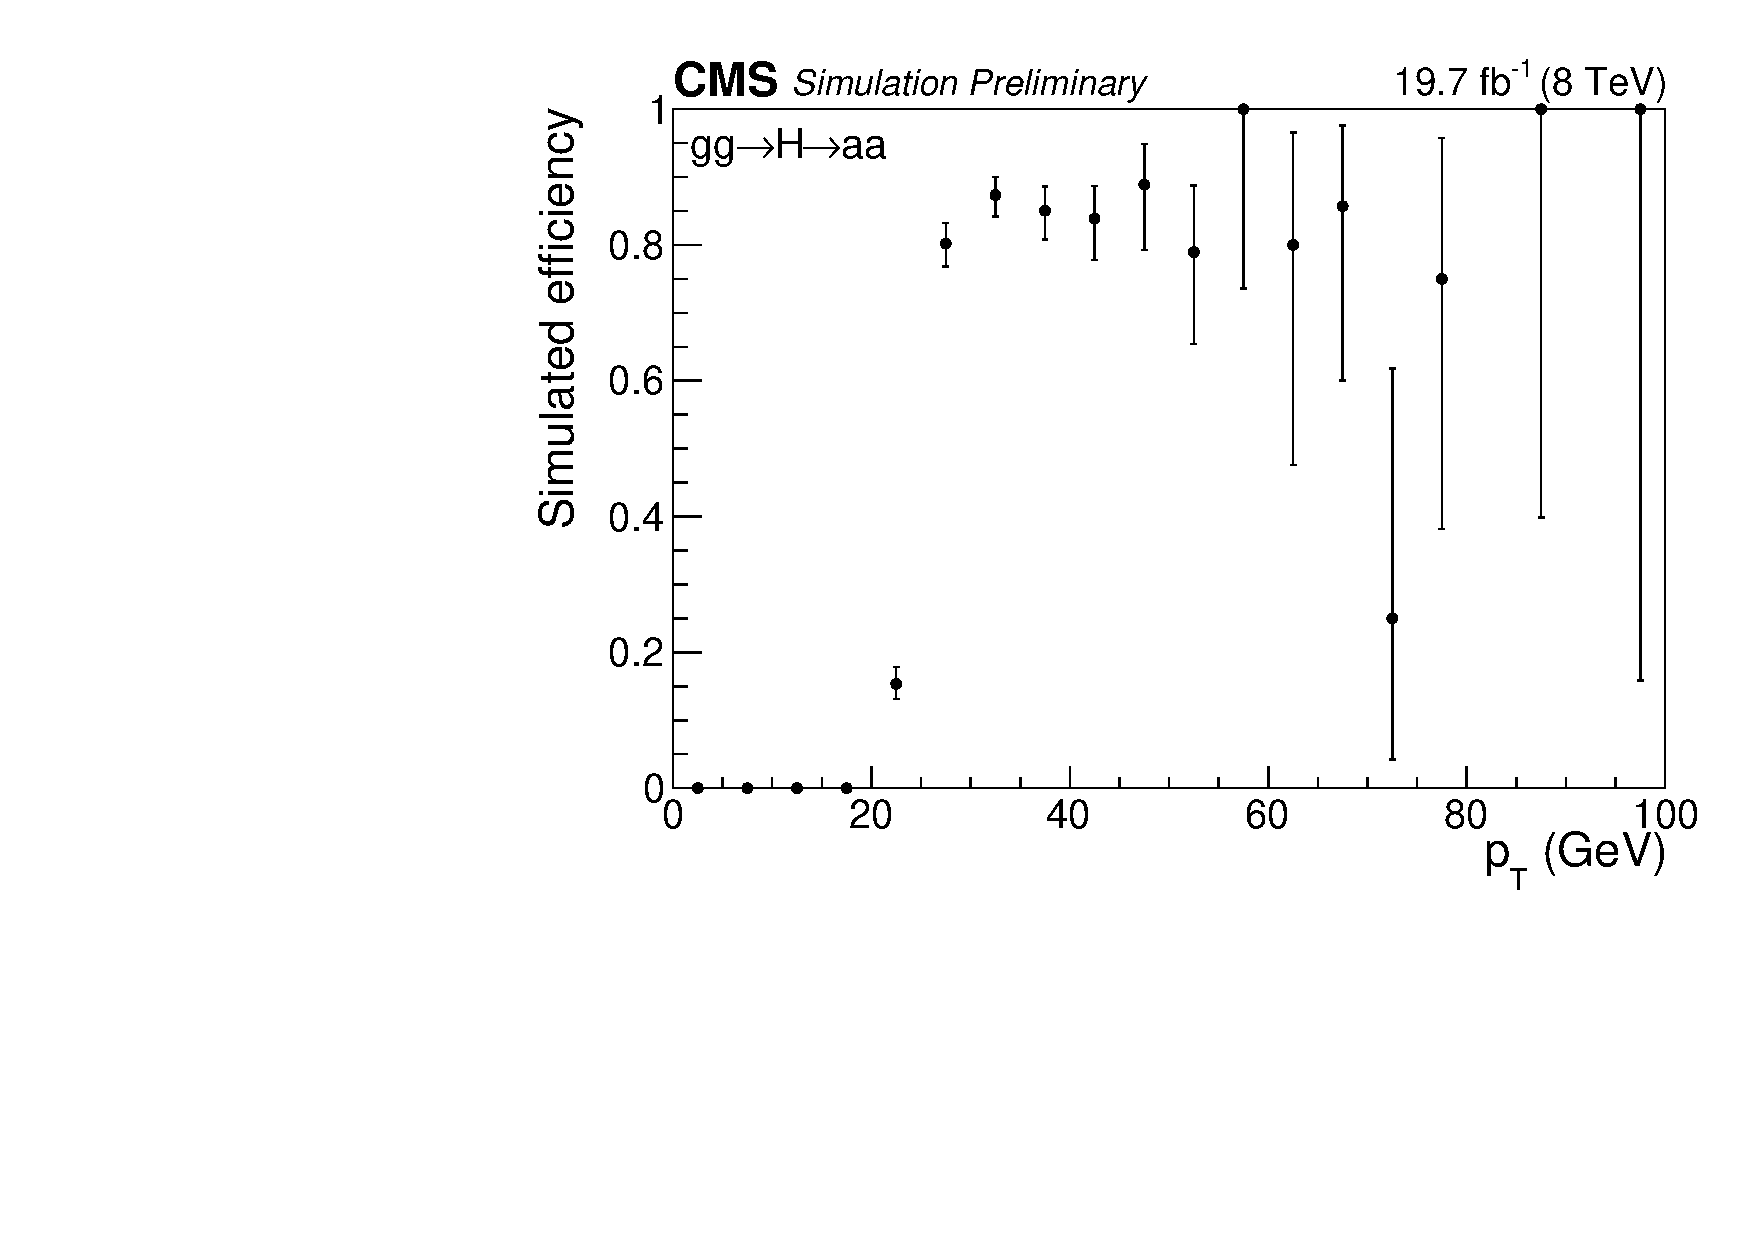
\includegraphics[width=1.24\cmsFigWidth]{figures/HLT_eff_Wmu_ggH}
    \caption{MC simulation prediction of efficiency for reconstructed muons passing the trigger muon ID to fire \texttt{HLT\_IsoMu24\_eta2p1}. Efficiencies were measured in MC events where the Higgs is produced via the (\cmsLeft) WH and (\cmsRight) gluon fusion channels.}
    \label{fig:HLT-eff-W-mu}
  \end{center}
\end{figure}

%Iso efficiency subsection
\subsection{Study of the particle flow relative isolation efficiency for signal events produced via gluon fusion\label{sec:muon-id-eff-iso}}

The efficiency for ggH $a\rightarrow\tau\rightarrow\mu$ decay muons that pass the tight muon ID criteria to pass the PF relative isolation cut is calculated for two reconstructed muon selections.  As a reminder, the PF relative isolation is defined as the $p_T$ sum of all PF hadrons and photons within a cone of $\Delta$R = 0.4 around the trigger muon divided by the trigger muon $p_T$.  Both selections have the PF relative isolation requirement of Sec.~\ref{sec:evtsel-triggermu} removed, since it is the efficiency of that requirement being studied here.   Barring that, the first selection is identical to the criteria described in Sec.~\ref{sec:evtsel-triggermu}, except that in addition the nearby lepton isolation requirement is removed.  Similarly, barring the PF relative isolation requirement, the second selection is identical to the criteria described in Sec.~\ref{sec:evtsel-triggermu}.  PF relative isolation efficiency is compared for the two selections.  Since the signature of pseudoscalar decays in the detector is similar between the ggH and VBF production modes, the results obtained for ggH simulation can be applied to VBF simulation as well.

The PF relative isolation efficiencies of the two selections are given by 

\begin{equation}
\epsilon_{\text{rel. iso}}^{\text{no }l\text{ iso}} = \frac{\text{No. gen-matched reco'd muons passing no-lepton-isolation ID and PF rel. iso.}}{\text{No. gen-matched reco'd muons passing trigger muon ID excl. PF rel. iso.}} \\
\label{eq:muonPFRelIsoeff-noliso}
\end{equation}

\begin{equation}
\epsilon_{\text{rel. iso.}} = \frac{\text{No. gen-matched reco'd muons passing trigger muon ID incl. PF. rel. iso.}}{\text{No. gen-matched reco'd muons passing trigger muon ID excl. PF rel. iso.}} \\
\label{eq:muonPFRelIsoeff}
\end{equation}

where

\begin{itemize}
\item the gen-matching criteria is $\Delta$$p_T$(reco muon, gen $a\rightarrow\tau\rightarrow\mu$ muon) $<$ 0.1 GeV and the gen muon is from the decay of a tau that is itself from the decay of a pseudoscalar;
\item the trigger muon ID for $\epsilon_{\text{rel. iso.}}^{\text{no }l\text{ iso}}$ is as described in Sec.~\ref{sec:evtsel-triggermu} but with the PF relative isolation and nearby lepton isolation requirements removed;
\item the trigger muon ID for $\epsilon_{\text{rel. iso.}}$ is as described in Sec.~\ref{sec:evtsel-triggermu} but with the PF relative isolation requirement removed; and
\item ``rel. iso.'' refers to passing the cut PF relative isolation $<$ 0.12.
\end{itemize}

Figure~\ref{fig:IsoEffVsDR} shows $\epsilon_{\text{rel. iso.}}^{\text{no }l\text{ iso}}$ as a function of $\Delta$R(gen $a\rightarrow\tau\rightarrow\mu$ muon, gen $\tau_{\text{2}}$), where the gen $a\rightarrow\tau\rightarrow\mu$ muon is matched to the reco'd muon as described in Eq.~\ref{eq:muonPFRelIsoeff-noliso} above and the gen $\tau_{\text{2}}$ is the other tau from the $a\rightarrow\tau\tau$ decay.  The efficiency is calculated separately for each decay mode of the gen $\tau_{\text{2}}$ (electronic, muonic, or hadronic).  $\epsilon_{\text{rel. iso.}}^{\text{no }l\text{ iso}}$ is $\sim$80\%, independent of $\Delta$R, for the $\tau_{\mu}\tau_{\text{e}}$ the $\tau_{\mu}\tau_{\mu}$ channels.  Because PF electrons and muons are not counted in the PF relative isolation sum, the presence of a nearby $\tau_{\text{e}}$ or $\tau_{\mu}$ does not significantly spoil the relative isolation of the main $a\rightarrow\tau\rightarrow\mu$ muon.  The overall efficiency is lower than the efficiency for $Z$ decay muons~\cite{1748-0221-7-10-P10002} by $\sim$15\% due to the different kinematics of di-tau objects vs. isolated $Z$ decay muons.  Conversely, in the $\tau_{\mu}\tau_{\text{had}}$ channel, $\epsilon_{\text{rel. iso.}}^{\text{no }l\text{ iso}}$ is $\sim$80\% only for $\Delta$R $>$ 0.4, when the two taus from pseudoscalar decay are separated enough that the tau decay muon appears isolated.  When the two taus are closer than $\Delta$R $\sim$ 0.4, the efficiency decreases because the hadronically decaying non-identified partner tau spoils the relative isolation of the tau decay muon that is identified as a trigger muon.

\begin{figure}[hbtp]
  \begin{center}
    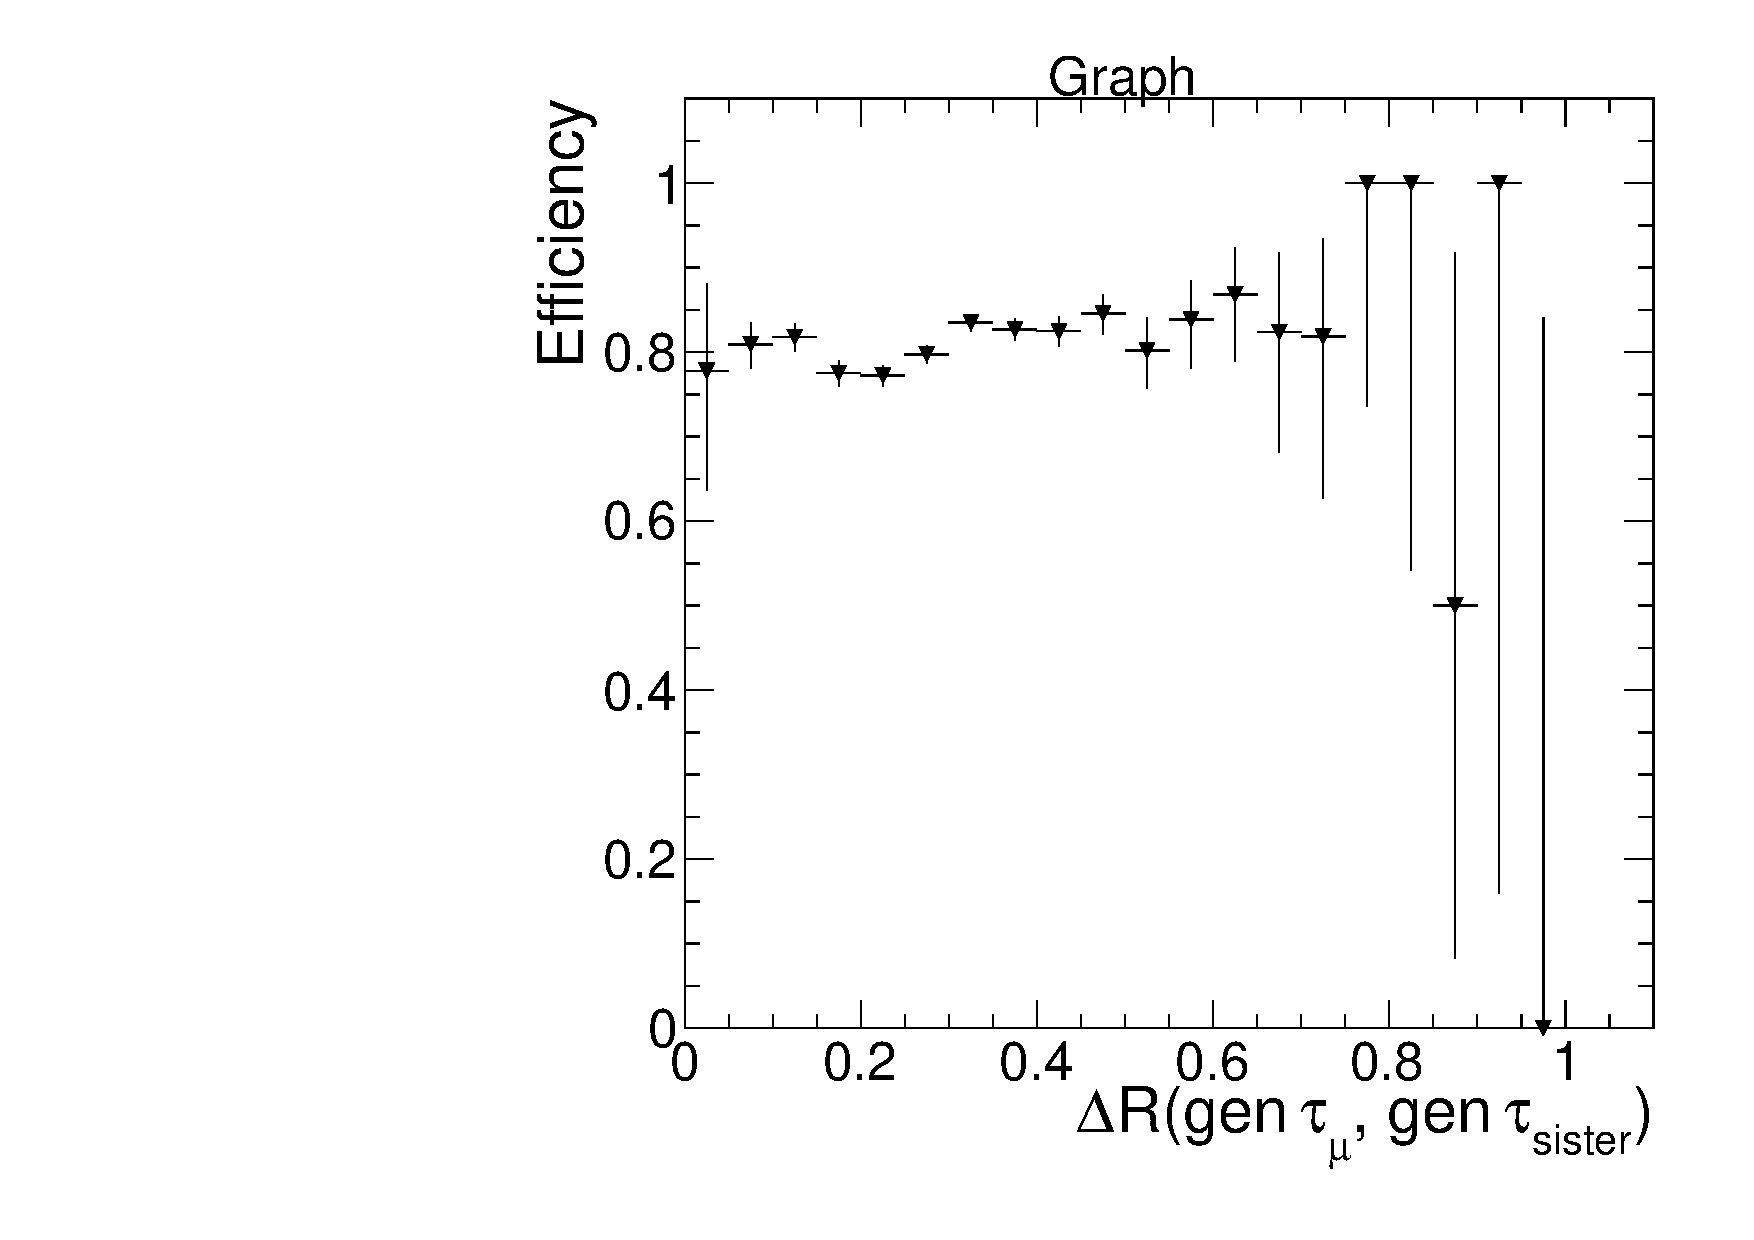
\includegraphics[width=0.8\cmsFigWidth]{figures/dRIsoEfficiency_muEOnly}
    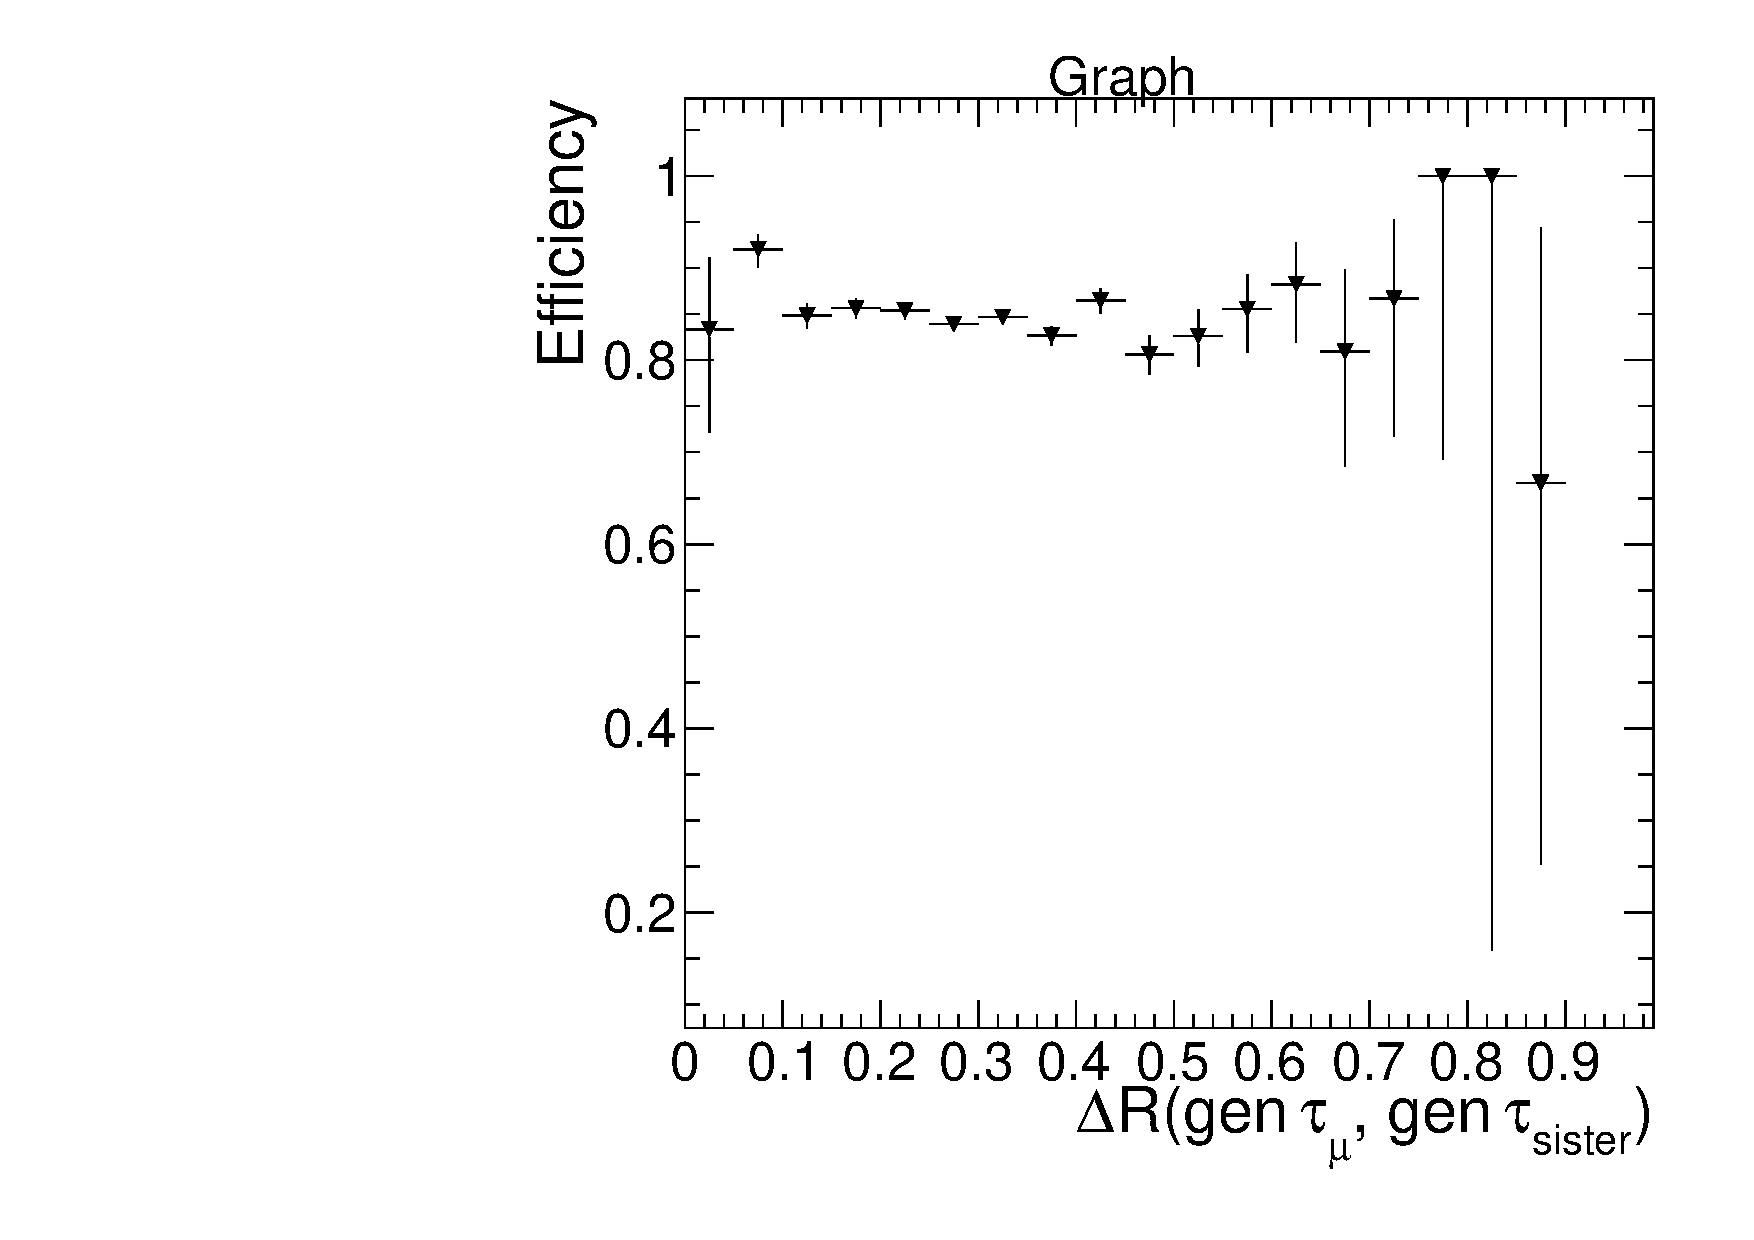
\includegraphics[width=0.8\cmsFigWidth]{figures/dRIsoEfficiency_muMuOnly}
    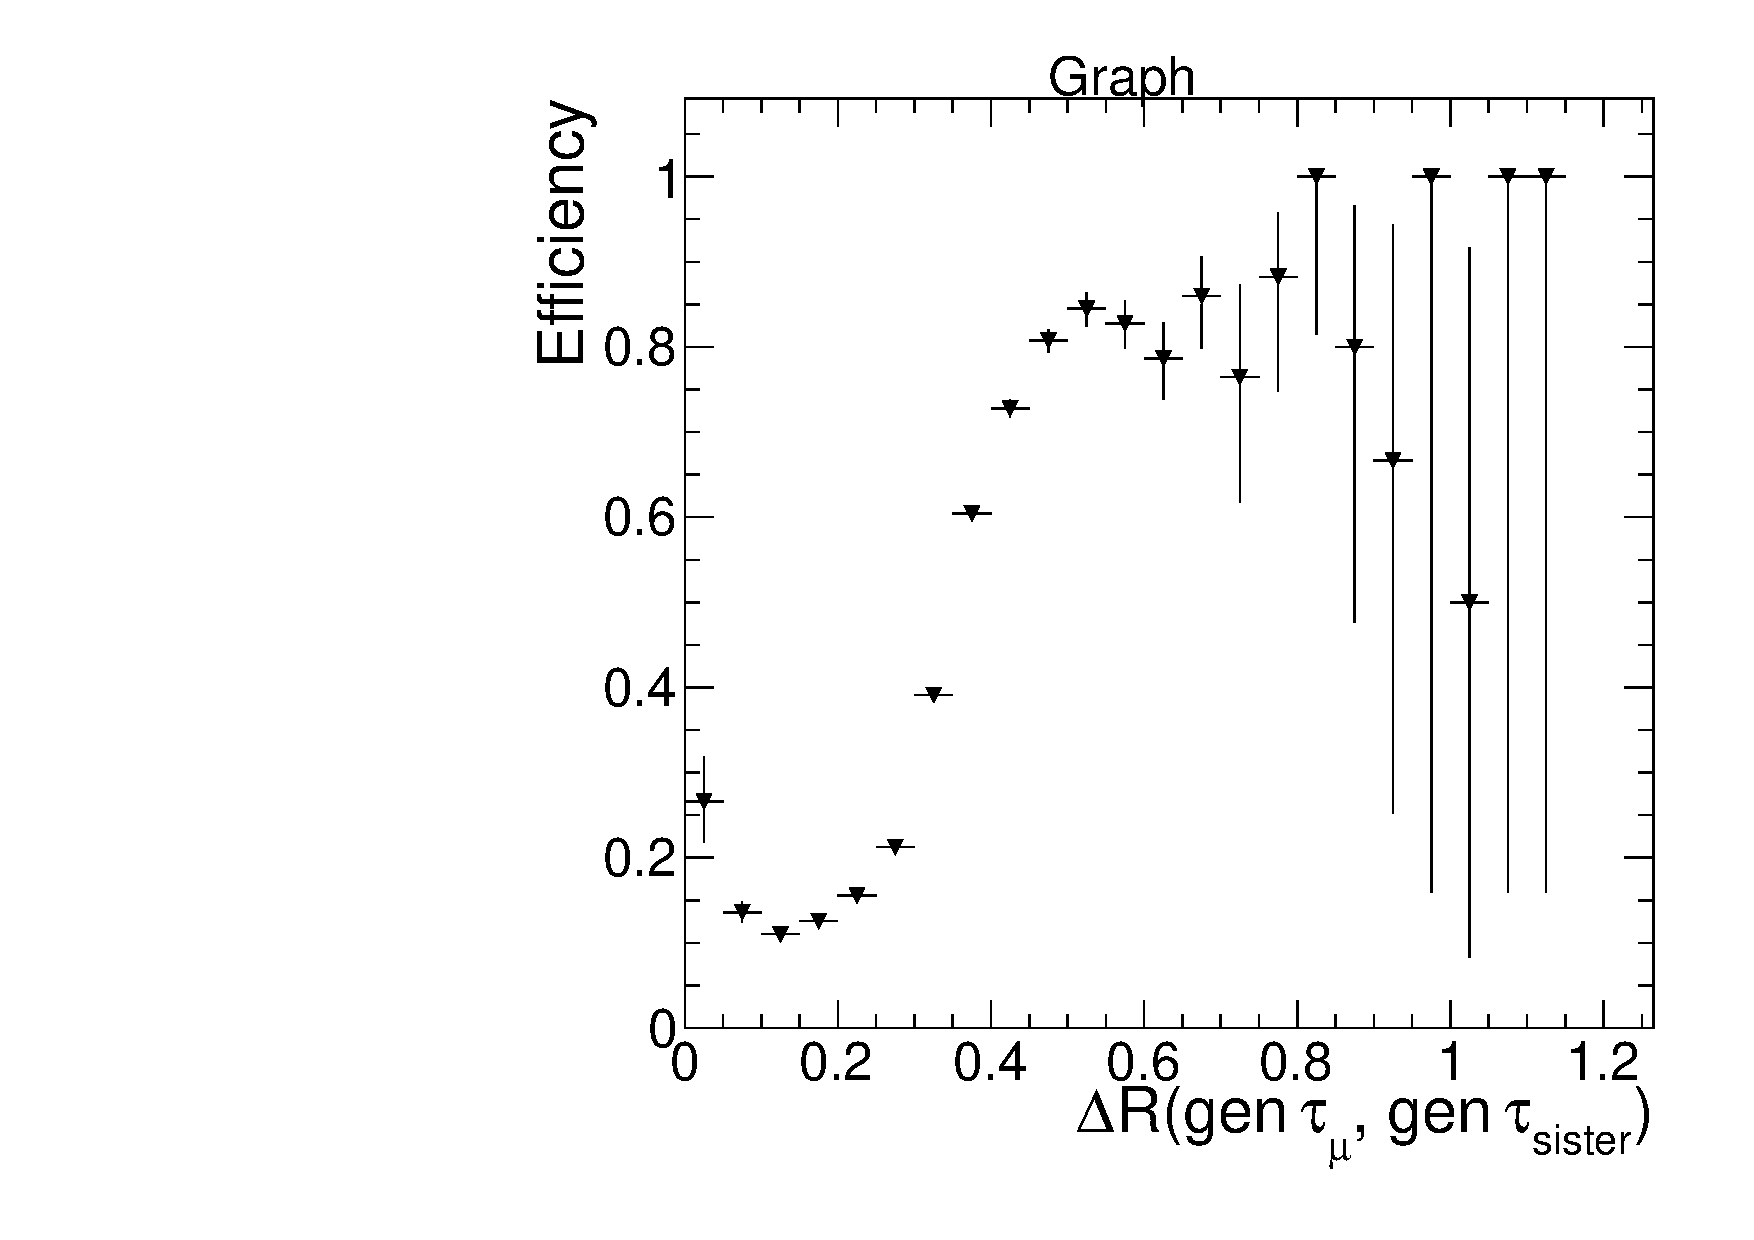
\includegraphics[width=0.8\cmsFigWidth]{figures/dRIsoEfficiency_muHadOnly}
    \caption{$\epsilon_{\text{rel. iso.}}^{\text{no }l\text{ iso}}$ for the ggH signal as a function of the separation $\Delta$R(gen $a\rightarrow\tau\rightarrow\mu$ muon, gen $\tau_{\text{2}}$), where the gen $\tau_{\text{2}}$ is a decay product of the same pseudoscalar as in the $a\rightarrow\tau\rightarrow\mu$.  The $a\rightarrow\tau\rightarrow\mu$ muon is matched to the reco'd muon as described in the text.  The reco'd muon is required to pass the trigger muon ID of Sec.~\ref{sec:evtsel-triggermu}, but with the PF relative isolation (because this is the cut under study) and nearby lepton isolation requirements removed.  (\cmsLeft) Gen $\tau_{\text{2}}$ decays to an electron.  (middle) Gen $\tau_{\text{2}}$ decays to a muon.  (\cmsRight) Gen $\tau_{\text{2}}$ decays to hadrons.}
    \label{fig:IsoEffVsDR}
  \end{center}
\end{figure}

In contrast, Figure~\ref{fig:IsoEffVsDR_withFilters} shows $\epsilon_{\text{rel. iso.}}$ as a function of $\Delta$R(gen $a\rightarrow\tau\rightarrow\mu$ muon, gen $\tau_{\text{2}}$), where the gen $a\rightarrow\tau\rightarrow\mu$ muon is matched to the reco'd muon as described in Eq.~\ref{eq:muonPFRelIsoeff} above and the gen $\tau_{\text{2}}$ is the other tau from the $\cmsSymbolFace{a}\rightarrow\tau\tau$ decay.  The efficiency is calculated separately for each decay mode of the gen $\tau_{\text{2}}$ (electronic, muonic, or hadronic).  The efficiencies are much flatter in $\Delta$R\ when the nearby lepton isolation requirement is applied to the reconstructed trigger muon, because it ensures that events can pass the selection sequence only if the two reconstructed taus from the pseudoscalar decay are well separated.  The PF relative isolation efficiency for $a\rightarrow\tau\rightarrow\mu$ muons in these events is now similar to that of $Z$ decay muons and is in the regime where the trigger muon is isolated and MC describes the data well.

\begin{figure}[hbtp]
  \begin{center}
    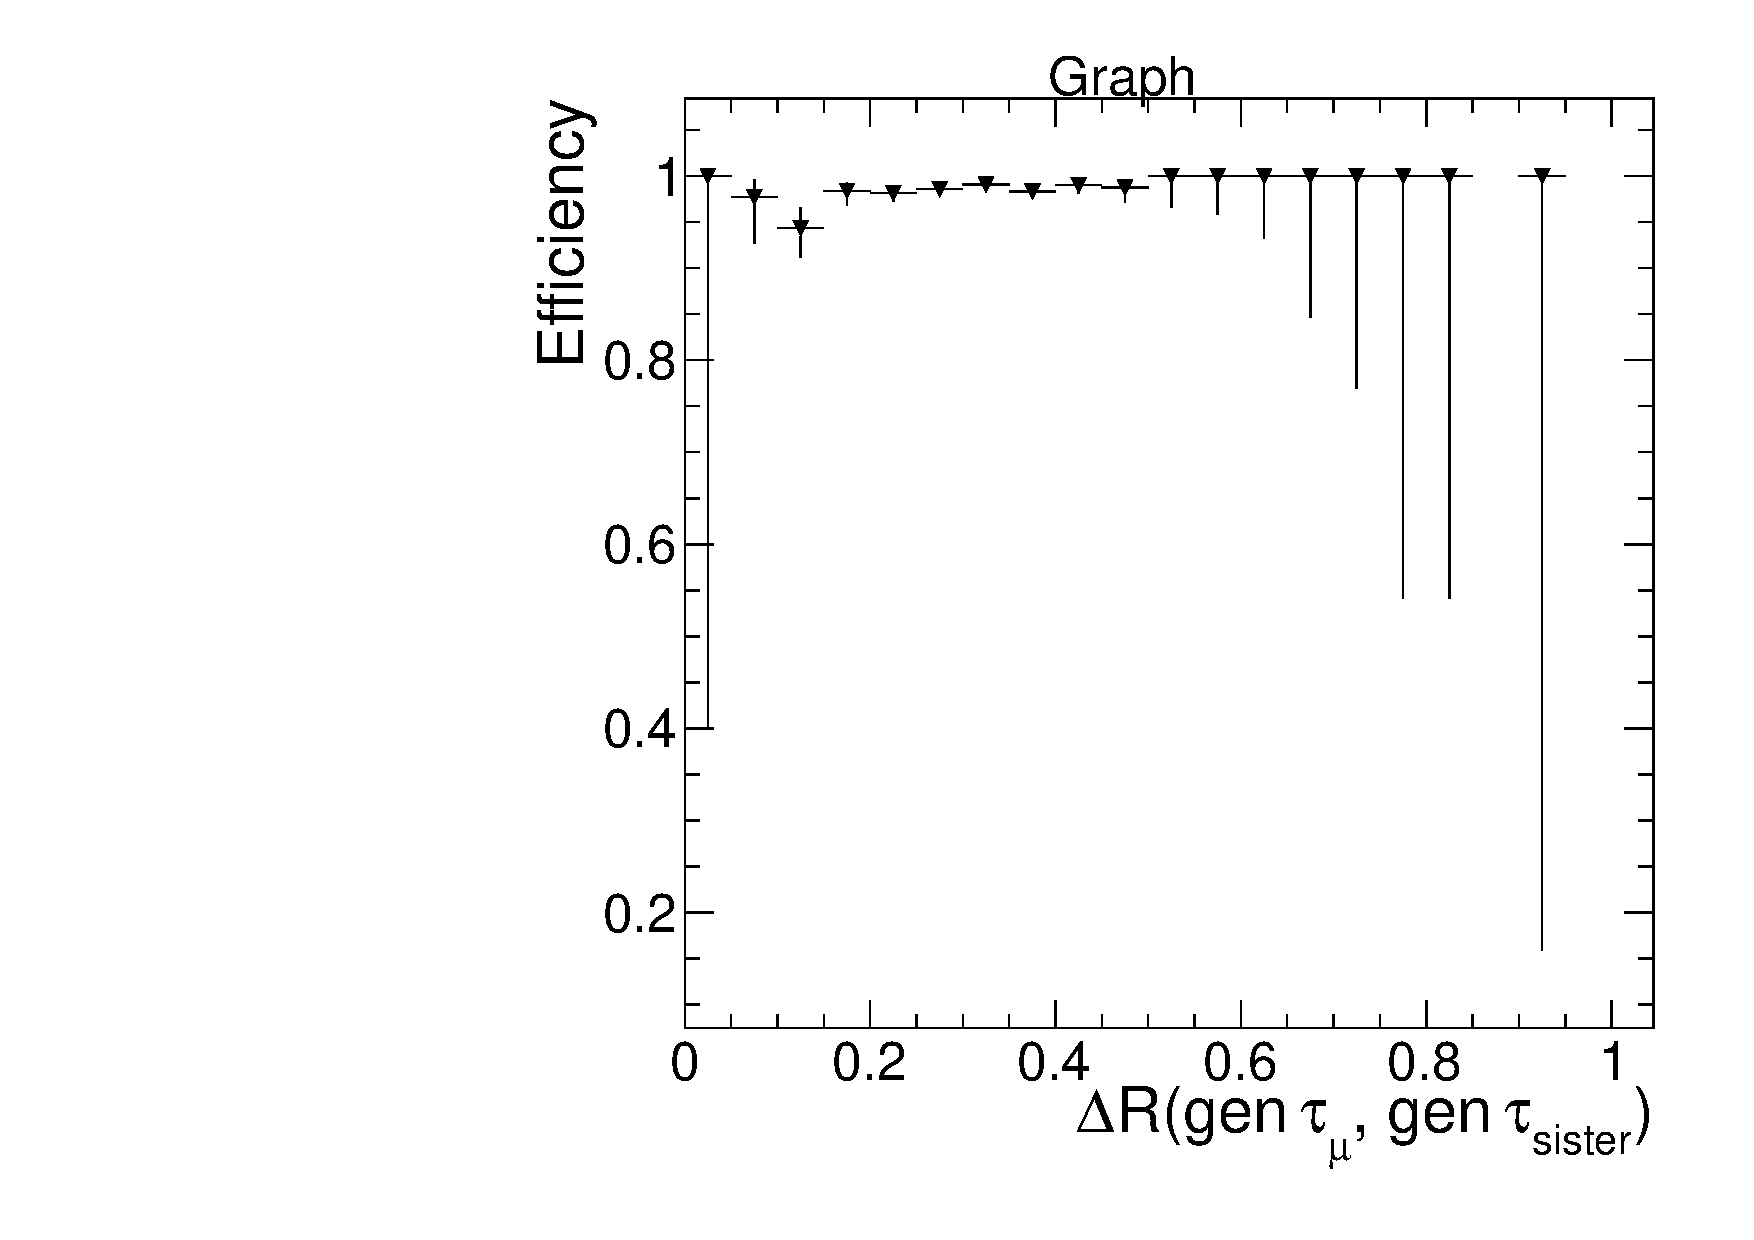
\includegraphics[width=0.8\cmsFigWidth]{figures/dRIsoEfficiency_withFilters_muEOnly}
    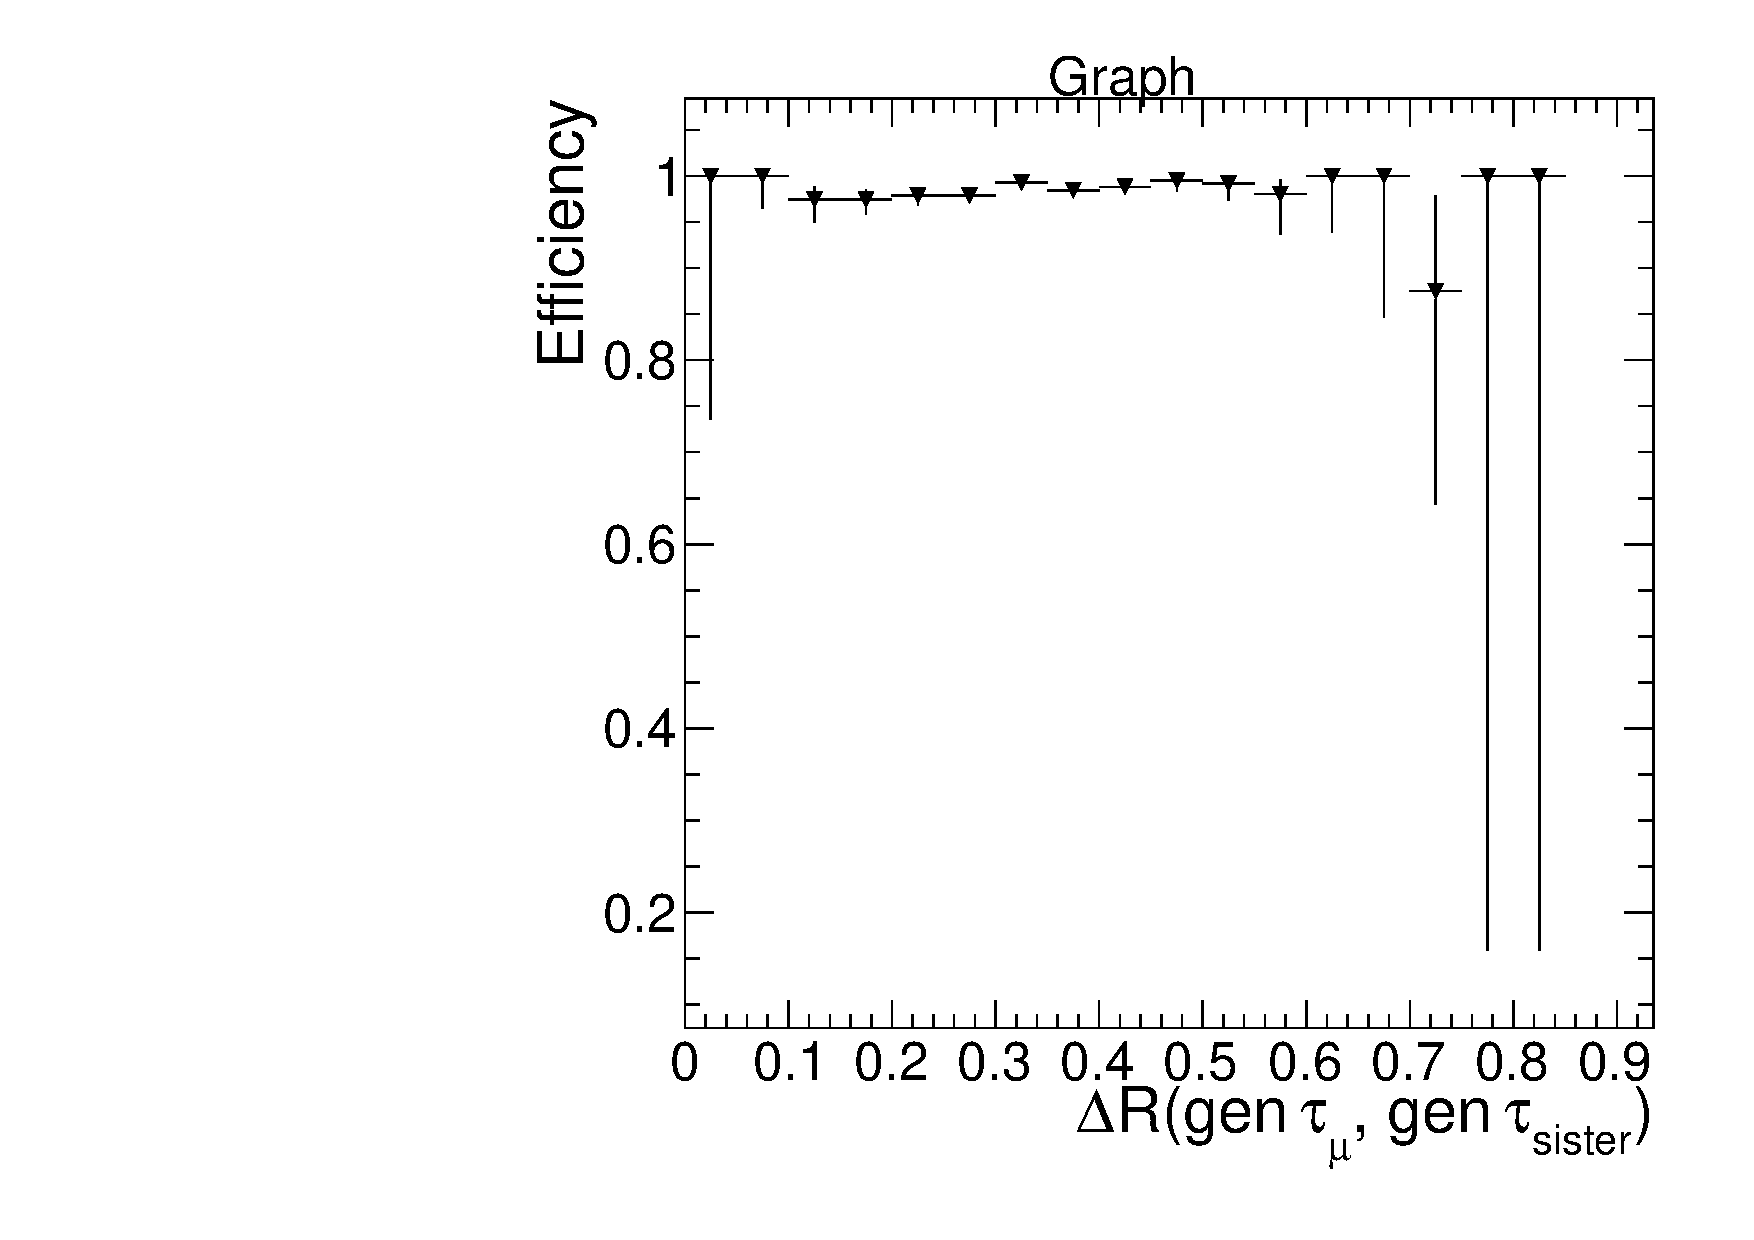
\includegraphics[width=0.8\cmsFigWidth]{figures/dRIsoEfficiency_withFilters_muMuOnly}
    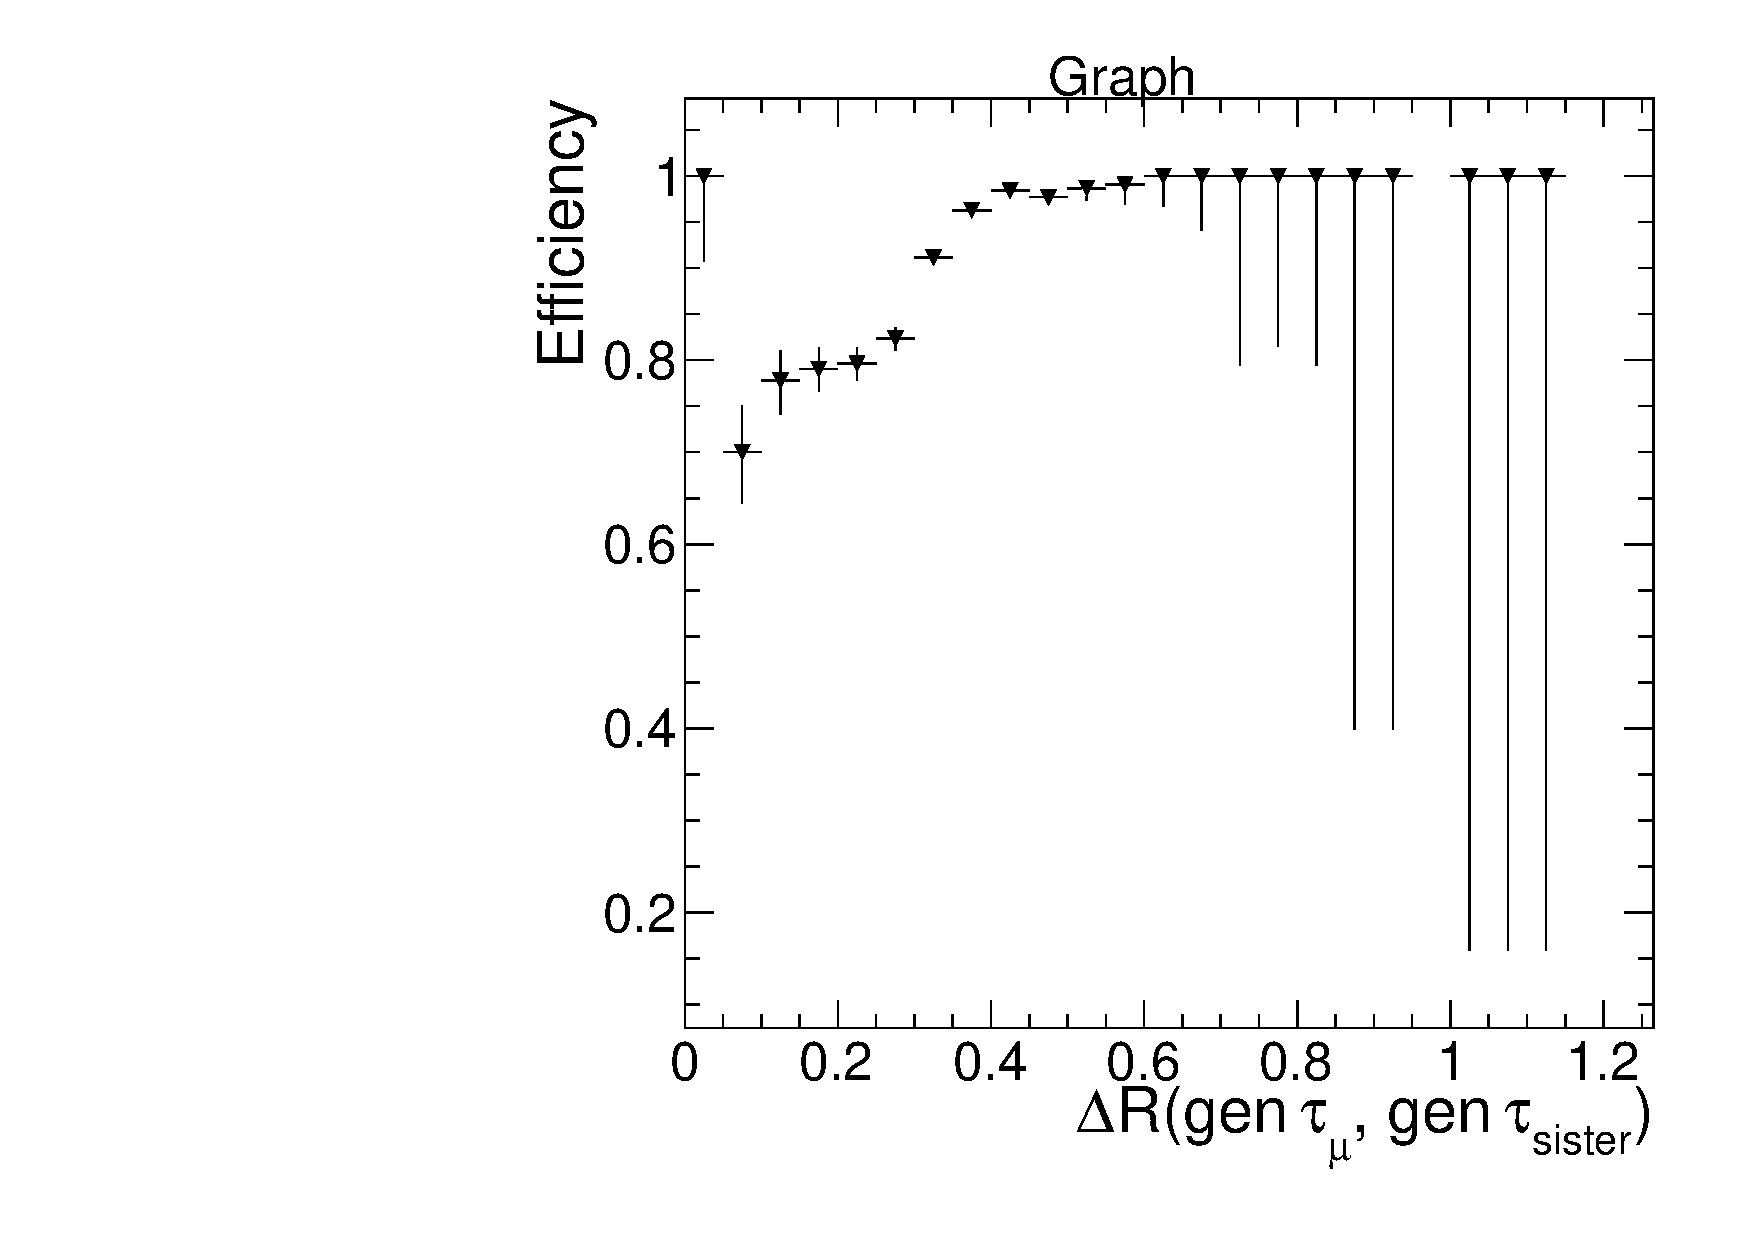
\includegraphics[width=0.8\cmsFigWidth]{figures/dRIsoEfficiency_withFilters_muHadOnly}
    \caption{$\epsilon_{\text{rel. iso.}}$ for the ggH signal as a function of the separation $\Delta$R(gen $a\rightarrow\tau\rightarrow\mu$ muon, gen $\tau_{\text{2}}$), where the gen $\tau_{\text{2}}$ is a decay product of the same pseudoscalar as in the $a\rightarrow\tau\rightarrow\mu$.  The $a\rightarrow\tau\rightarrow\mu$ muon is matched to the reco'd muon as described in the text.  The reco'd muon is required to pass the trigger muon ID of Sec.~\ref{sec:evtsel-triggermu}, but with the PF relative isolation requirement removed (because this is the cut under study).  (\cmsLeft) Gen $\tau_{\text{2}}$ decays to an electron.  (middle) Gen $\tau_{\text{2}}$ decays to a muon.  (\cmsRight) Gen $\tau_{\text{2}}$ decays to hadrons.}
    \label{fig:IsoEffVsDR_withFilters}
  \end{center}
\end{figure}

After all other selection cuts, the acceptance of the nearby lepton isolation requirement ranges from 87\% to 95\% for ggH pseudoscalar masses 7, 9, 11, 13, and 15 GeV.

%boosted tau ID
\section{Boosted tau ID\label{sec:evtsel-ditau}}

The target signature in this search is one in which one of the $a$ decays results in a $\tau_{\mu}\tau_{\text{had}}$ final state, while no constraints are placed on the decay of the taus coming from the other $\cmsSymbolFace{a}$. The hadronic tau identification algorithm employed in this search is the HPS algorithm.

As described in Section~\ref{sec:semileptonic}, the tau pairs produced in the pseudoscalar decays will be highly collimated, and their decay products will invade one another's isolation cones. In particular, for the $\tau_{\mu}\tau_{\text{had}}$ pair, the muon from $\tau_{\mu}$ has been found to end up frequently among the constituents of the jet seeded by the $\tau_{\text{had}}$ decay and therefore among the isolation constituents of the $\tau_{\text{had}}$ reconstructed with HPS.  Figure~\ref{fig:evt-sel-HPS-iso-eff-standard-vs-boosted-ID} shows the $\tau_{\text{had}}$ isolation efficiency for the standard HPS ID versus the boosted $\tau_{\mu}\tau_{\text{had}}$ ID described below.  The isolation efficiency is about four times higher for the boosted $\tau_{\mu}\tau_{\text{had}}$ ID.

\begin{figure}[hbtp]
  \begin{center}
    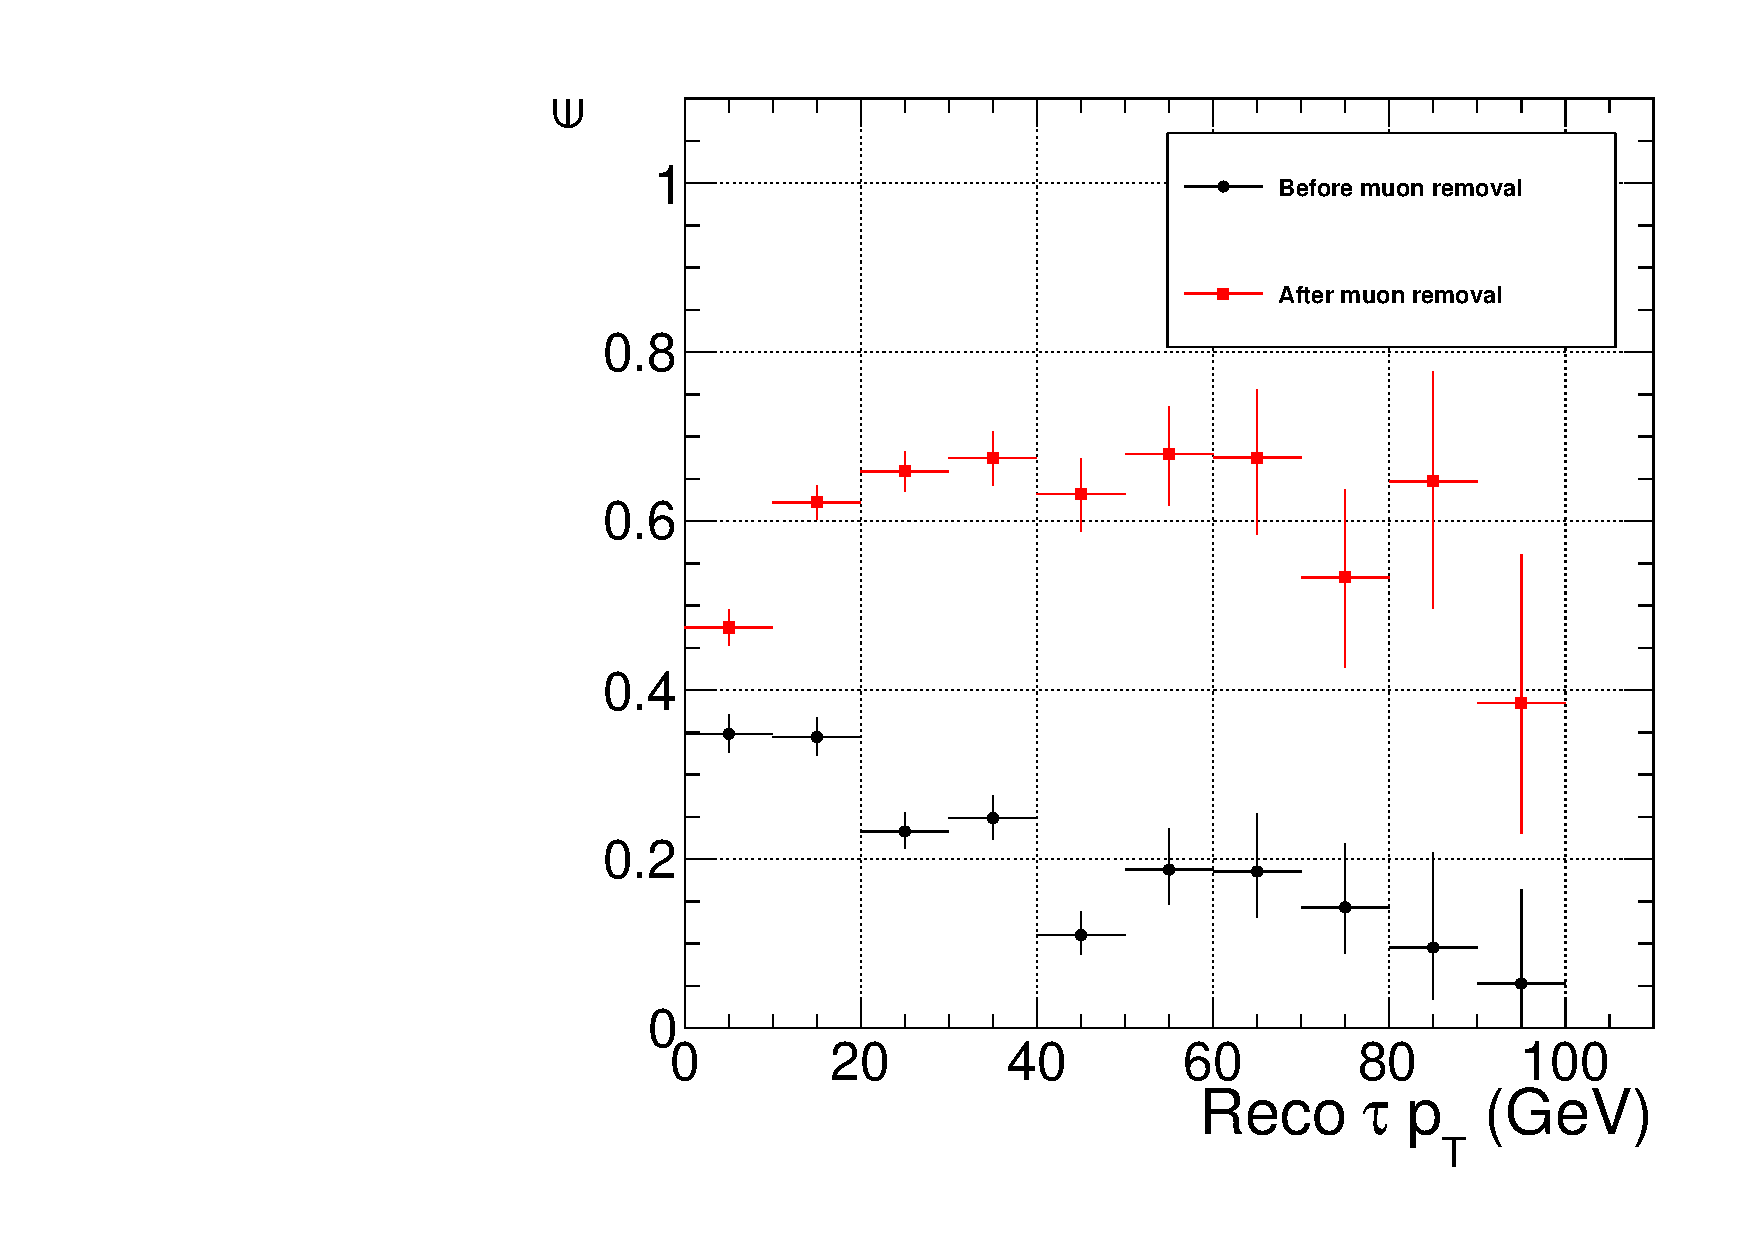
\includegraphics[width=\cmsFigWidth]{figures/effVsPT_MCTruthMuonRemoval_LooseCombinedIsolationDBSumPtCorr_canvas}
    \caption{Hadronic tau isolation efficiency for the WH signal using the standard tau identification algorithm (black) and the boosted ID developed for this search (red).}
    \label{fig:evt-sel-HPS-iso-eff-standard-vs-boosted-ID}
  \end{center}
\end{figure}

To recover the correct reconstruction of the $\tau_{\text{had}}$, a method has been developed to identify soft muon candidates for the $\tau_{\mu}$ and remove them from the constituents of any jet that contained them, while the remaining jet constituents are then reconstructed into a jet and passed to the HPS algorithm to reconstruct a $\tau_{\text{had}}$ decay. The MUO POG soft muon ID is used to identify $\tau_{\mu}$ candidates.

%soft mu
\subsection{Soft muon ID\label{sec:evtsel-softmu}}

In addition to the trigger $\mu$ requirement, events are selected that have at least one reco muon passing the following cuts:
\begin{itemize}
	\item $p_T >$ 5 GeV
	\item $\abs{\eta} <$ 2.4
%	\item required to be \DR \textgreater 0.3 from the reco muon identified earlier as the $\PW_{\mu}$ (thus excluding the possibility that the $\tau_{\mu}$ and $\PW_{\mu}$ candidates are the same object)
	\item Distinct from the trigger muon
	\item Soft muon ID~\cite{CMS:2010uta}:
	\begin{itemize}
		\item Tracker muon track is matched with at least one muon segment in both \unit{x} and y coordinates
		\item More than 5 tracker layers with hits
		\item Number of pixel layers $>$ 1
		\item The tracker muon track fit has $\chi^{2}/\text{ndof} <$ 1.8
		\item The reco muon's tracker track has $d_{\text{xy}} <$ 3 mm and $d_{\text{z}} <$ 30 mm
	\end{itemize}
\end{itemize}
After all soft muons passing these requirements are collected, they are used as described in Section~\ref{sec:evtsel-tauID} to reconstruct $\tau_{\text{had}}$ objects.

%Jet cleaning and boosted tau ID
\subsection{Jet cleaning and hadronic tau ID\label{sec:evtsel-tauID}}

In this search, tau decays are reconstructed from the anti-$k_{\text{T}}$ R = 0.5~\cite{1126-6708-2008-04-063} PF jets (``ak5PFJets'') using the HPS algorithm. Before running HPS, jet constituents passing the soft muon ID (Sec.~\ref{sec:evtsel-softmu}) are removed. In the majority of cases, only one soft muon is removed from a jet, but if more than one muon is removed, the highest $p_T$ removed muon is identified as the $\tau_{\mu}$. A new ak5PFJet (henceforth referred to as the cleaned jet after the removal of the muon) is then reconstructed from the remaining PF constituents. These cleaned jets are submitted to the HPS algorithm and reconstructed as $\tau_{\text{had}}$ candidates.

The event is then selected to have at least one $\tau_{\text{had}}$ candidate reconstructed as above with $p_T >$ 20 GeV, $\abs{\eta} <$ 2.3, and passing the HPS \texttt{DecayModeFinding} and \texttt{\\MediumCombinedIsolationDBSumPtCorr} discriminators. HPS is currently capable of reconstructing the following hadronic tau decay modes: single hadron (one prong decay, or one prong plus one low-energy $\pi^0$), single hadron plus one ECAL strip (one prong plus one $\pi^0$), single hadron plus two strips (one prong plus one $\pi^0$ in which the photons from the $\pi^0$ decay are well separated in the ECAL), and three hadrons (three prong decay). In addition, because no anti-muon or anti-electron discriminators are applied to the HPS object, some leptonic tau decays get counted as single hadron decays.  The DecayModeFinding discriminator requires that the reconstructed HPS $\tau_{\text{had}}$ object have one of these four decay modes. Further selection on the isolation of the $\tau_{\text{had}}$ candidate helps to discriminate against fake taus reconstructed from quark or gluon jets, which tend to involve more hadronic activity and soft radiation and thus are less isolated.  The HPS isolation energy, described in \cite{CMS_AN_2010-082}, is defined by the $\Delta\beta$ pileup-corrected $E_T$ sum of the PF charged and neutral hadron and PF gamma candidates found within a $\Delta$R = 0.5 cone around the $\tau_{\text{had}}$ axis.  The \texttt{MediumCombinedIsolationDBSumPtCorr} discriminator~\cite{CMS:tauidtwiki} imposes an upper limit of 1.0 GeV on the HPS isolation energy.

In the majority of events passing all these selection cuts, there is only one $\tau_{\text{had}}$ passing both HPS discriminators after the $\tau_{\mu}$ is removed from the jet used to reconstruct it. If more than one $\tau_{\text{had}}$ object passes, then the one with the highest $p_T$ is taken to be the $\tau_{\text{had}}$. If more than one $\tau_{\mu}\tau_{\text{had}}$ object is found in the event, the one with the highest $\tau_{\mu}\tau_{\text{had}}$ invariant mass is chosen.

Only one $\tau_{\mu}\tau_{\text{had}}$ object is selected in this search. Requiring two such objects was tested, to see whether this could increase sensitivity to the WH signal, but this was observed to kill all MC background events, while only a handful of signal events and QCD control sample events survived.  It would have been impossible to model the background meaningfully.

%charge requirements
\section{Opposite charge muon veto\label{sec:evtsel-OSSF}}

The presence of two muons in the event, one of which is isolated and energetic, makes Drell-Yan di-muon production a large background.  To combat this, the trigger $\mu$ and $\tau_{\mu}$ are required to have the same electric charge.  Figures~\ref{fig:muHadMass_OSSFVeto_vs_none_lowMT} and~\ref{fig:muHadMass_OSSFVeto_vs_none_highMT} show the effect of this requirement on the Drell-Yan background, which is reduced by almost a factor of 20 in the low-$M_{T}$ bin and 13 in the high-$M_{T}$ bin, at a cost of reducing the signal by at most 50\%.

\begin{figure}[hbtp]
  \begin{center}
    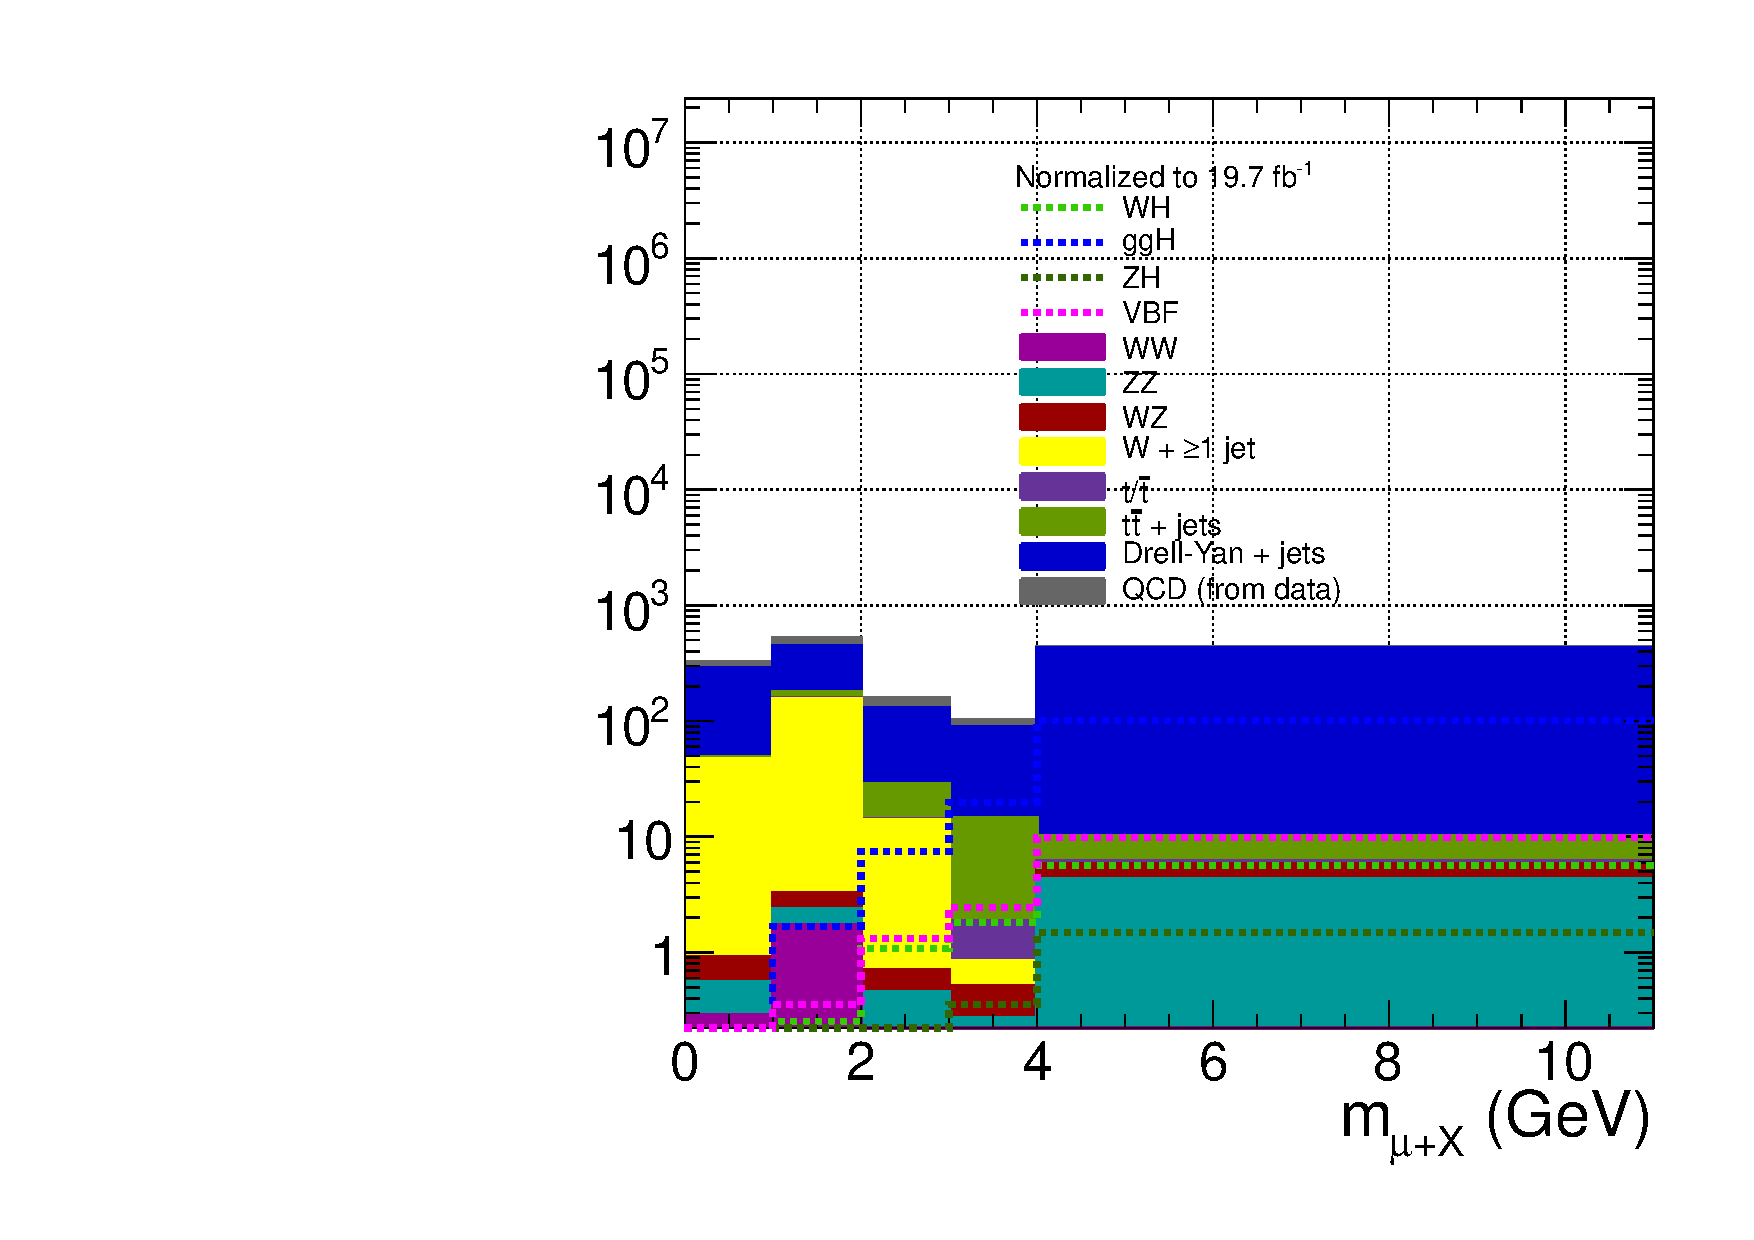
\includegraphics[width=1.2\cmsFigWidth]{figures/muHadMass_lowMT_beforeOSSF}
    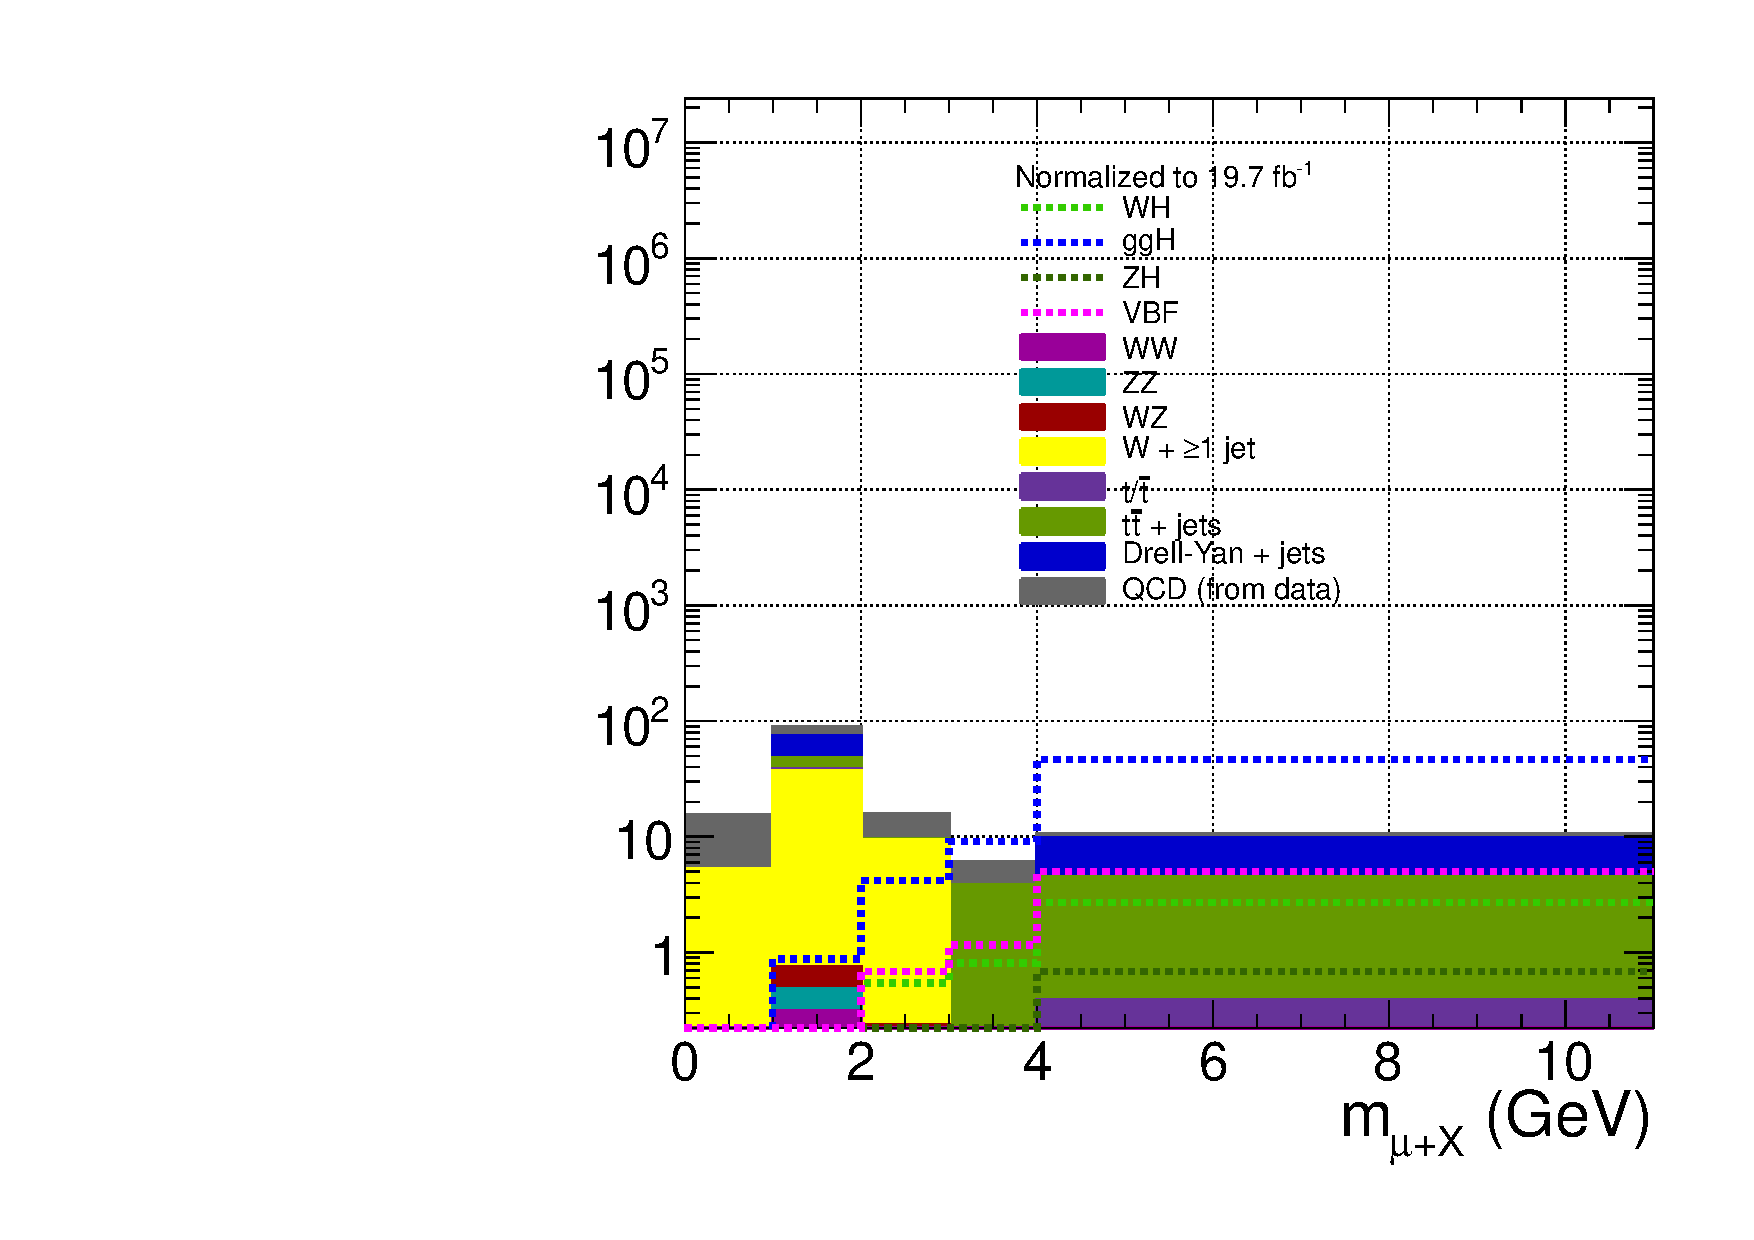
\includegraphics[width=1.2\cmsFigWidth]{figures/muHadMass_lowMT_afterOSSF}
    \caption{Invariant mass of the $\tau_{\mu}\tau_{\text{had}}$ pair for signals in the low-$M_{T}$ bin with $m_a$ = 9 GeV and all backgrounds before (\cmsLeft) and after (\cmsRight) the (trigger $\mu$)-$\tau_{\mu}$ same charge requirement.  All backgrounds except QCD are estimated from MC simulation. }
    \label{fig:muHadMass_OSSFVeto_vs_none_lowMT}
  \end{center}
\end{figure}

\begin{figure}[hbtp]
  \begin{center}
    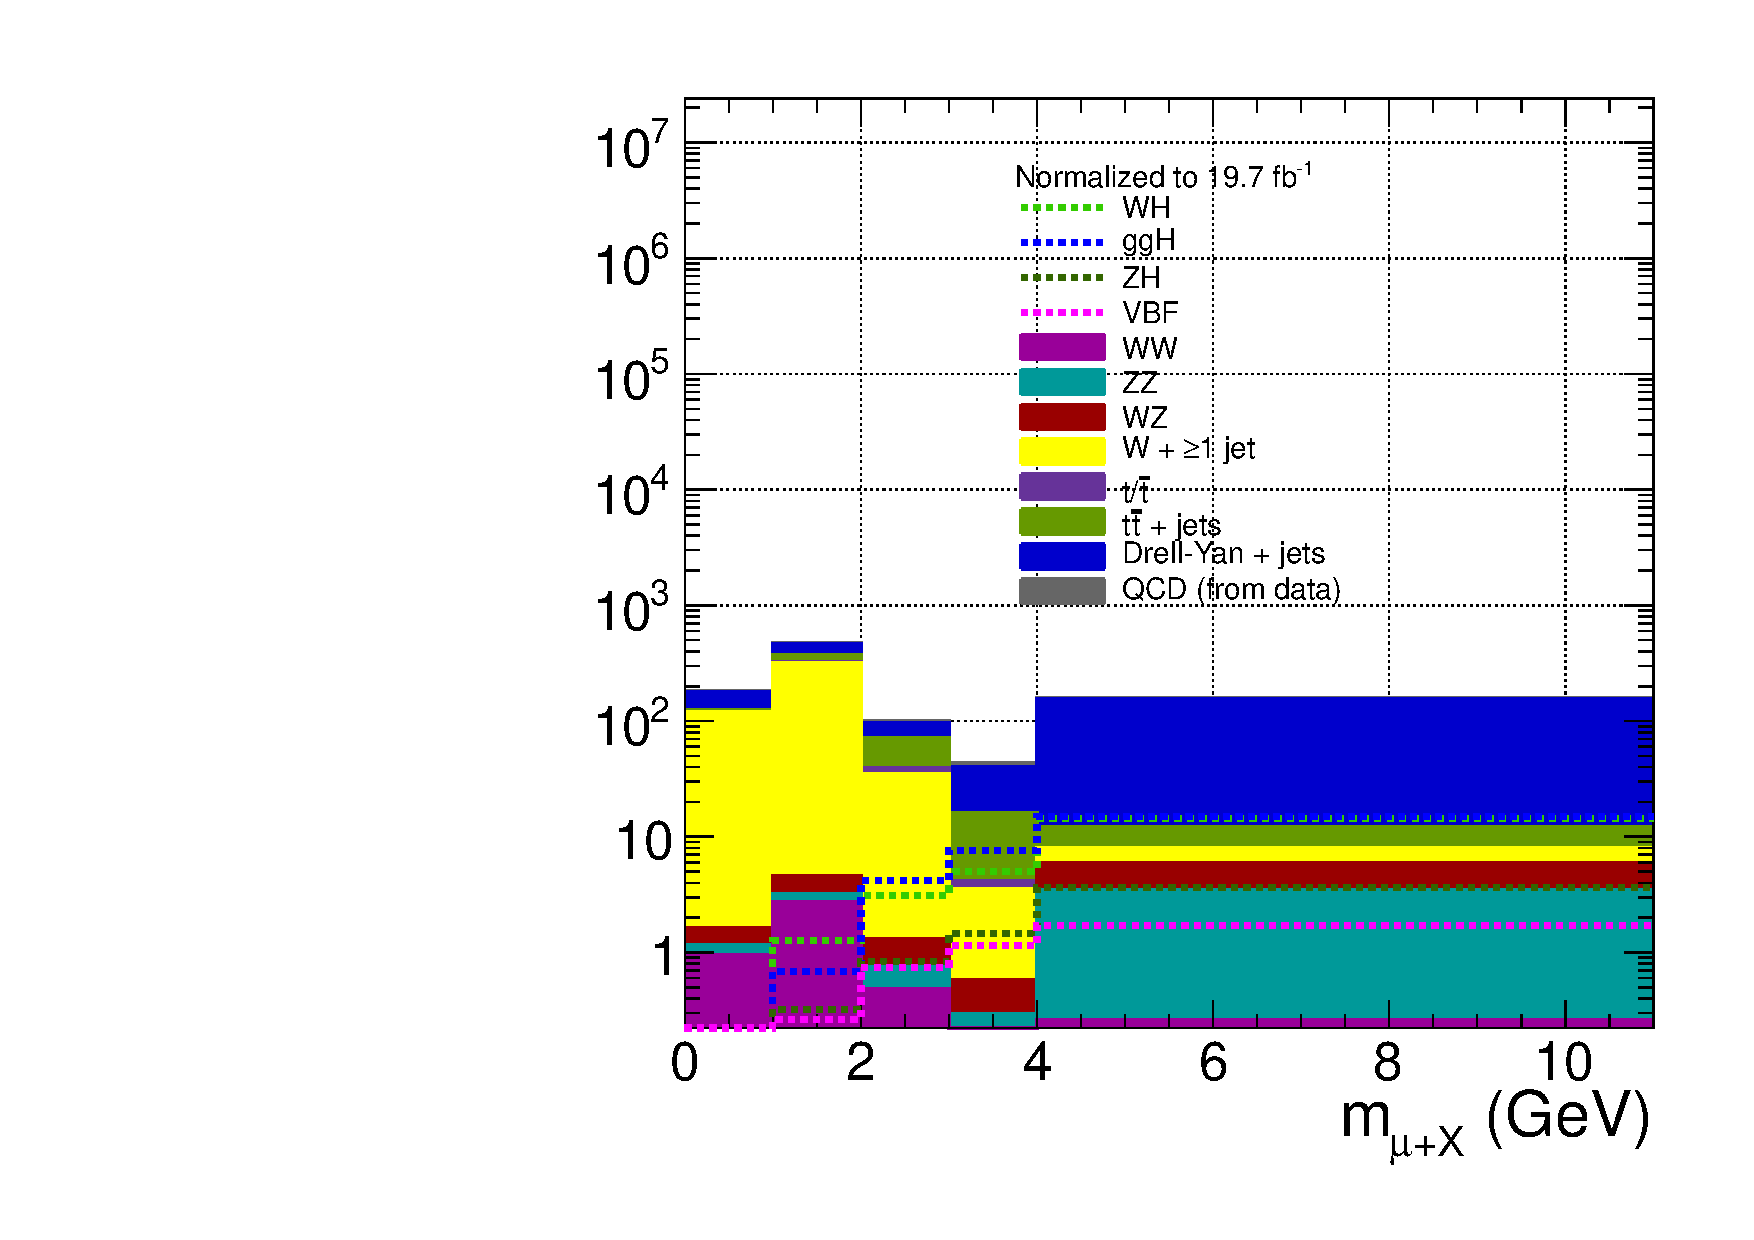
\includegraphics[width=1.2\cmsFigWidth]{figures/muHadMass_highMT_beforeOSSF}
    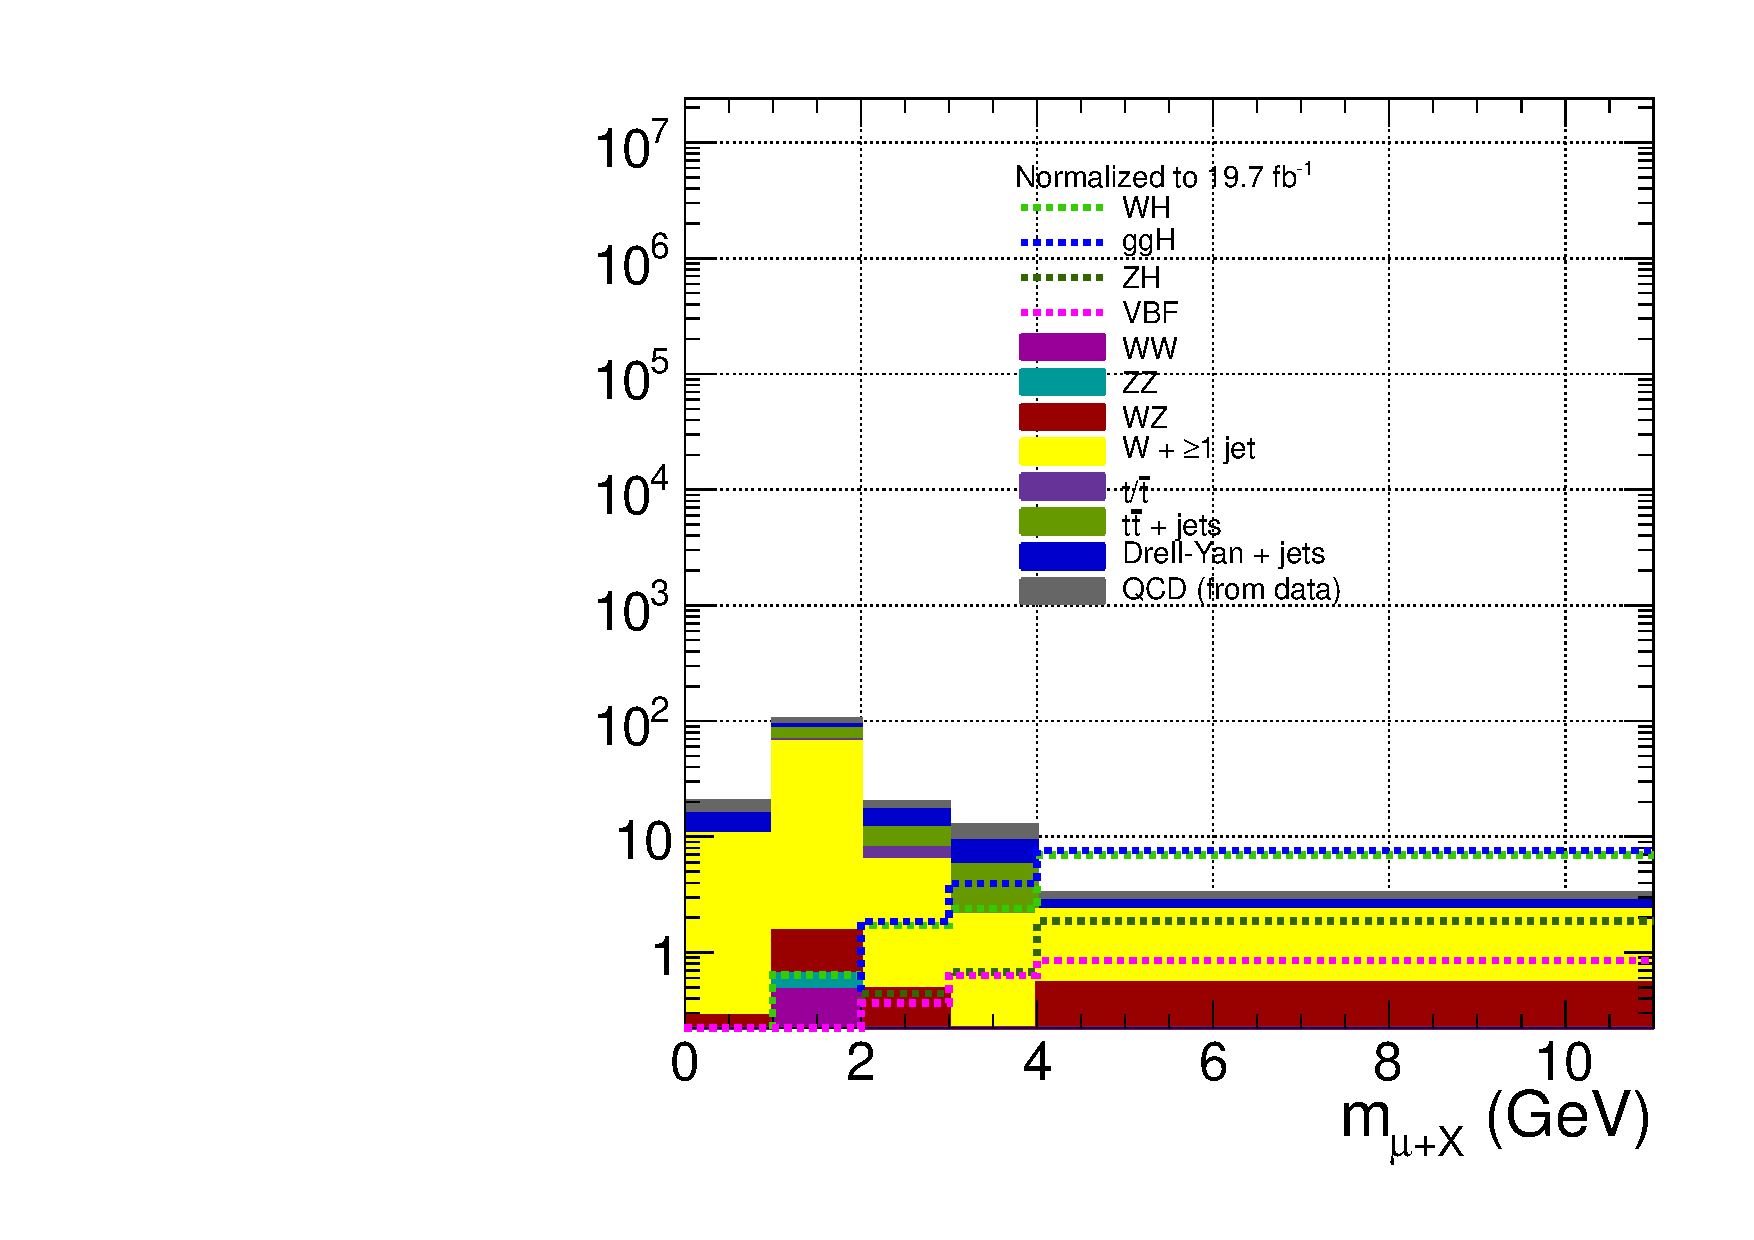
\includegraphics[width=1.2\cmsFigWidth]{figures/muHadMass_highMT_afterOSSF}
    \caption{Invariant mass of the $\tau_{\mu}\tau_{\text{had}}$ pair in the high-$M_{T}$ bin for signals with $m_a$ = 9 GeV and all backgrounds before (\cmsLeft) and after (\cmsRight) the (trigger $\mu$)-$\tau_{\mu}$ same charge requirement.  All backgrounds except QCD are estimated from MC simulation. }
    \label{fig:muHadMass_OSSFVeto_vs_none_highMT}
  \end{center}
\end{figure}

\section{Same charge tau veto\label{sec:evtsel-SSSF}}

$\tau_{\mu}\tau_{\text{had}}$ pairs are reconstructed in background events when there is a poorly isolated real muon, either promptly produced or coming from a heavy flavor jet, or when one track in a light jet fakes a soft muon and the others fake an HPS tau.  Fake $\tau_{\mu}\tau_{\text{had}}$ pairs rarely come from a real boosted di-tau decay, and therefore no correlation between the $\tau_{\mu}$ and $\tau_{\text{had}}$ charge is expected.  We therefore impose an opposite charge requirement on the $\tau_{\mu}$ and $\tau_{\text{had}}$, which reduces the background by about 20\% while leaving the signal virtually unchanged (Figure~\ref{fig:muHadMass_SSSF}).

\begin{figure}[hbtp]
  \begin{center}
    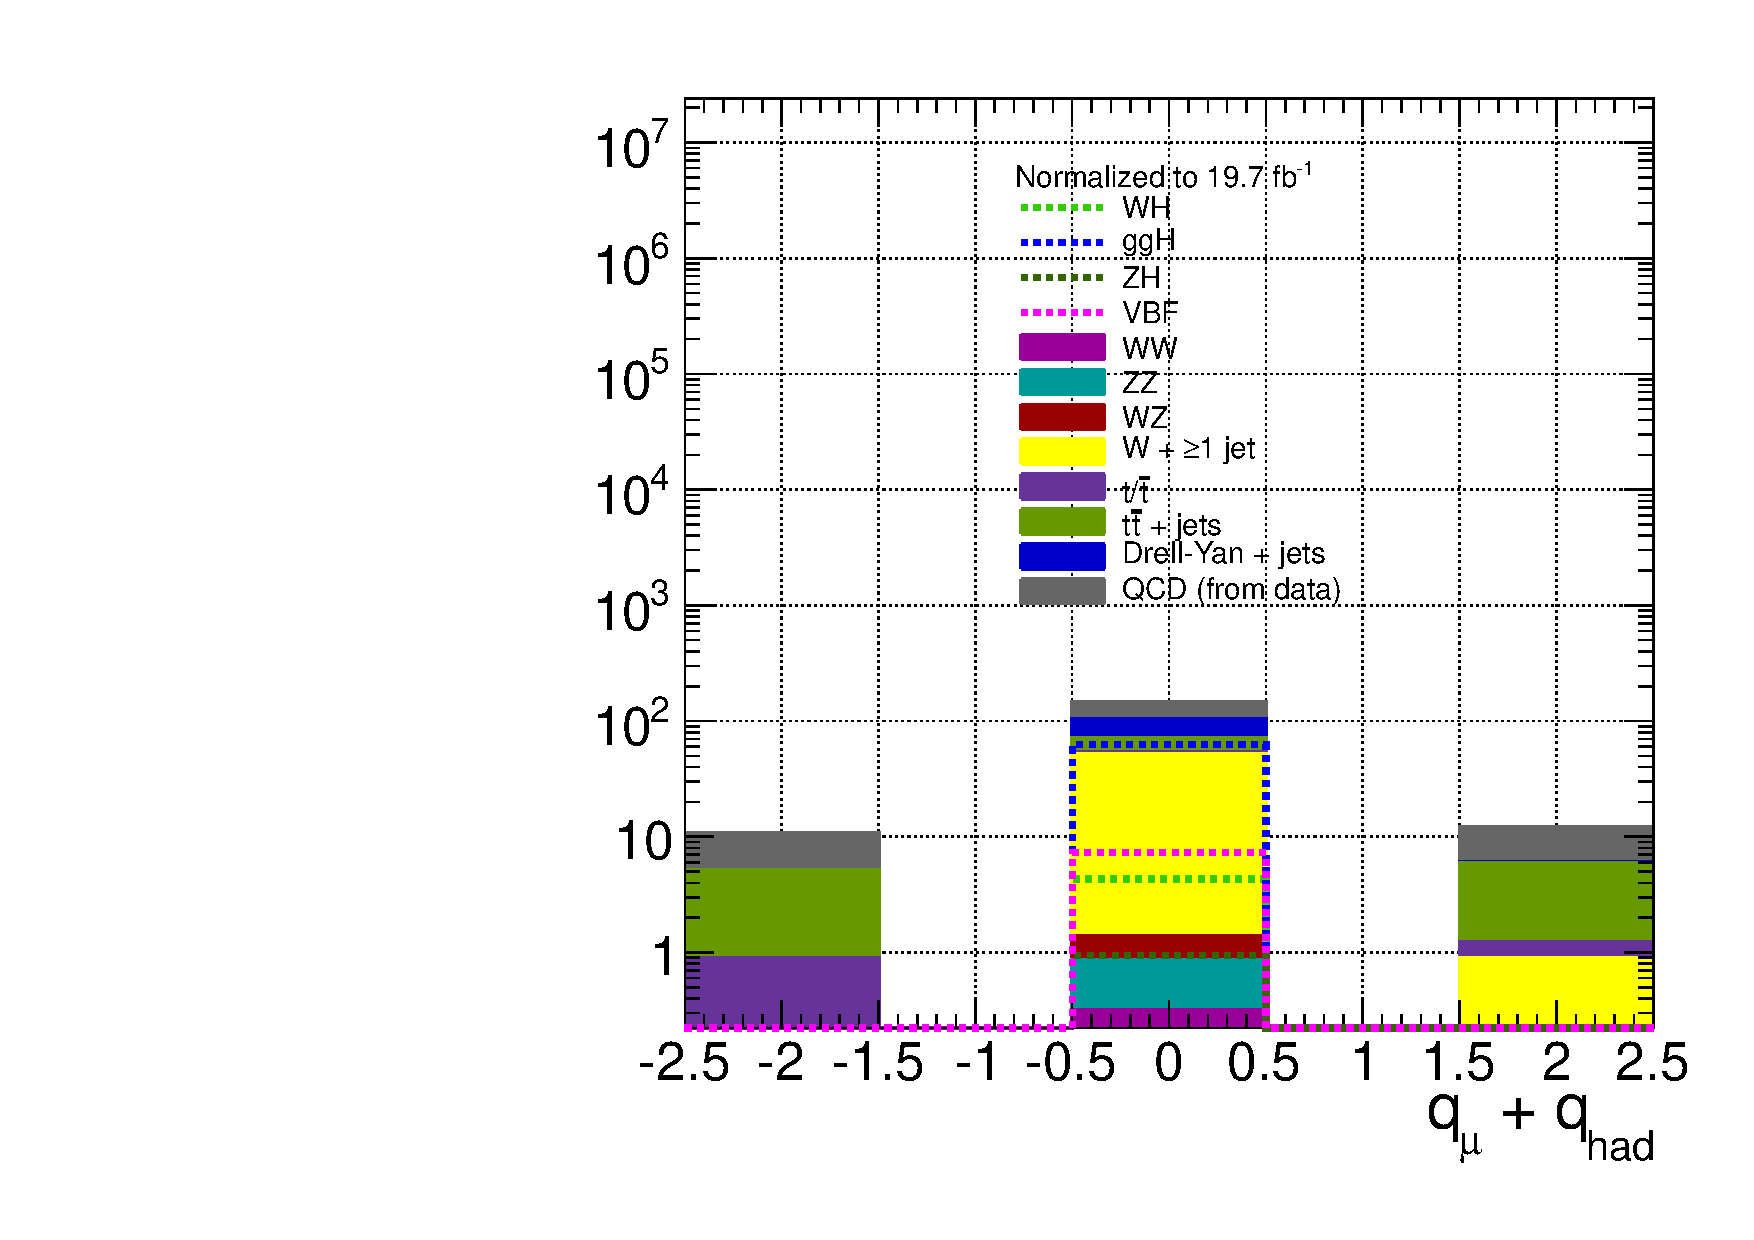
\includegraphics[width=1.2\cmsFigWidth]{figures/muHadCharge_lowMT_beforeSSSF}
    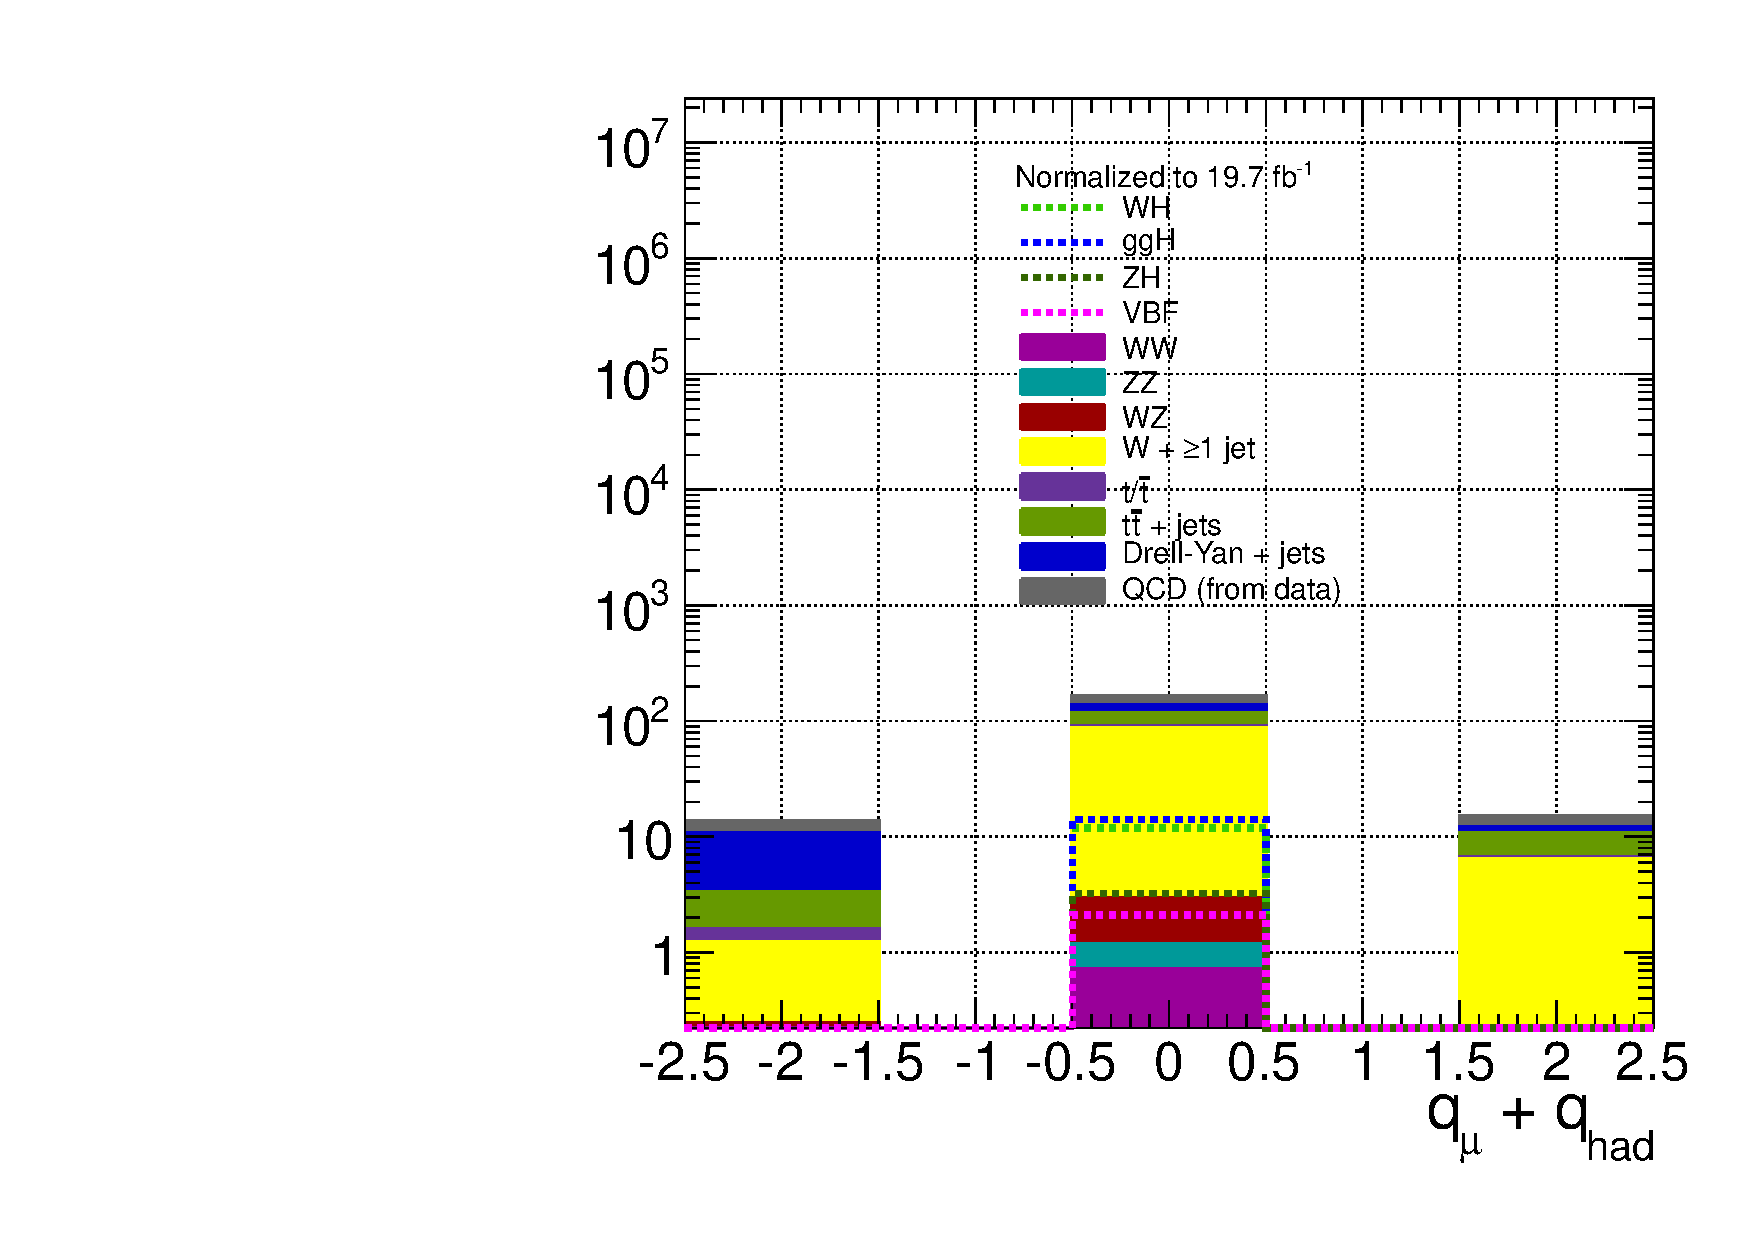
\includegraphics[width=1.2\cmsFigWidth]{figures/muHadCharge_highMT_beforeSSSF}
    \caption{Sum of the $\tau_{\mu}$ charge and $\tau_{\text{had}}$ charge for signals with $m_a$ = 9 GeV and all backgrounds.  All backgrounds except QCD are estimated from MC simulation. (\cmsLeft) Low-$M_{T}$ bin. (\cmsRight) High-$M_{T}$ bin. }
    \label{fig:muHadMass_SSSF}
  \end{center}
\end{figure}

%b-veto
\section{B-veto on tau jet\label{sec:evtsel-bveto}}

Heavy flavour jets, such as those from B meson or top decays, often contain a muon among the decay products which gets reconstructed as the $\tau_{\mu}$. Thus, the identification of b-jets can serve as a means to reject background from heavy flavour jets.

To optimize the identification of b-jets, b-tagging algorithms take advantage of the unique properties that distinguish b-jets from other kinds of jets produced at the LHC. One important property is the long lifetime of B mesons; when they decay, they will have travelled a significant distance (on the order of millimeters) from the primary vertex, resulting in displaced secondary vertices.  Thus, the impact parameter and secondary vertex associated with such jets can be used as discriminating variables. The combined secondary vertex (CSV) algorithm~\cite{Weiser:927399}, which is used in this search, employs a likelihood ratio that takes as input information about the primary vertex, secondary vertex, 2D and 3D impact parameters, track multiplicity, and track pseudorapidities of jets.

Figure~\ref{fig:sigVsBkg_csv_regA} shows the distribution of the CSV discriminator for Monte Carlo signals and all backgrounds except QCD in the low-$M_{\text{T}}$ and high-$M_{\text{T}}$ bins. As can be seen from this figure, the $\tau_{\text{had}}$ jet in the signal final states generally does not have large values of CSV; by vetoing b-tagged jets, the single top and $t\bar{t}$ backgrounds can be cut down significantly. A b-tag veto was thus implemented by rejecting events in which the cleaned jet associated with the $\tau_{\text{had}}$ object had a CSV value greater than the medium CSV working point of 0.679 recommended by the BTV POG for \texttt{22Jan2013} re-reco data at 8 \TeV~\cite{CMS:btvpogtwiki}.

\begin{figure}[hbtp]
  \begin{center}
    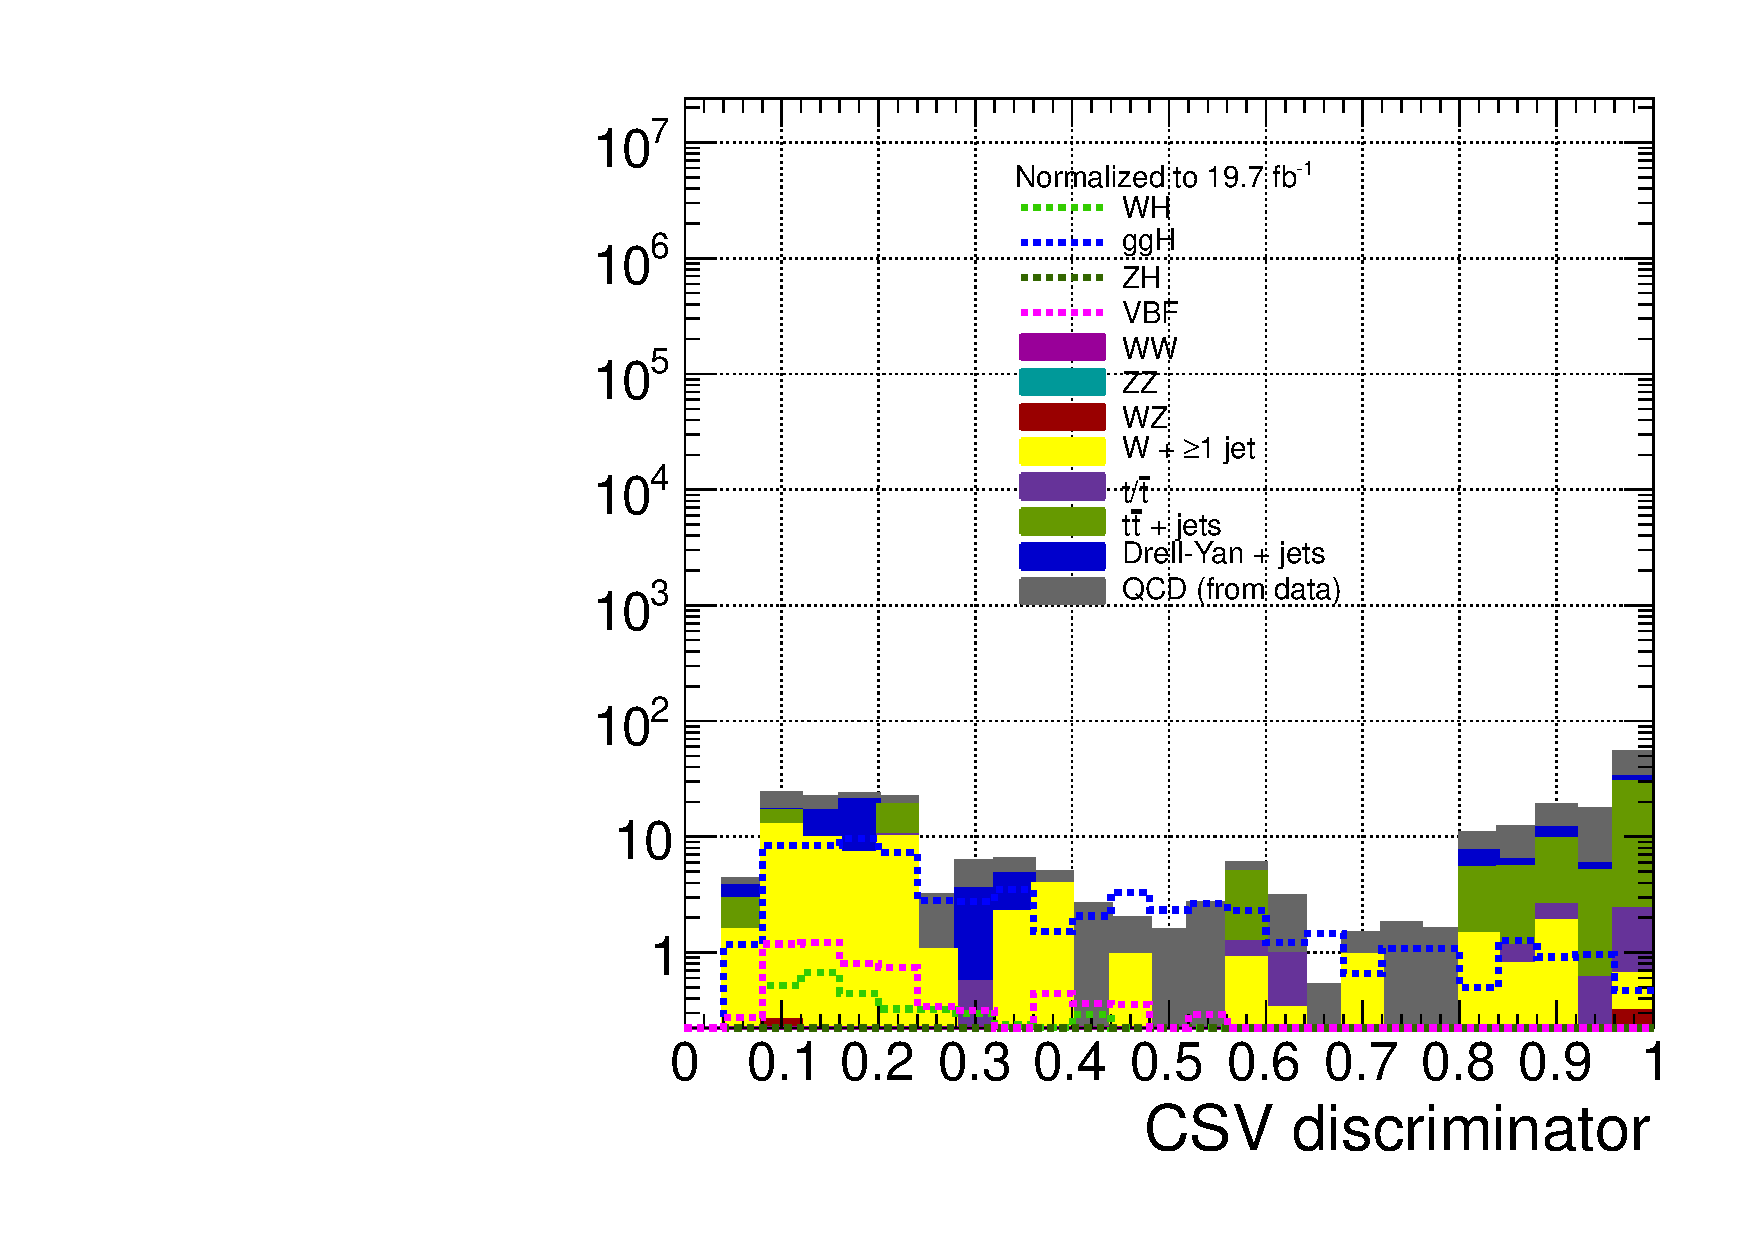
\includegraphics[width=\cmsFigWidth]{figures/sigVsBkg_csv_regA_lowMT_v61}
    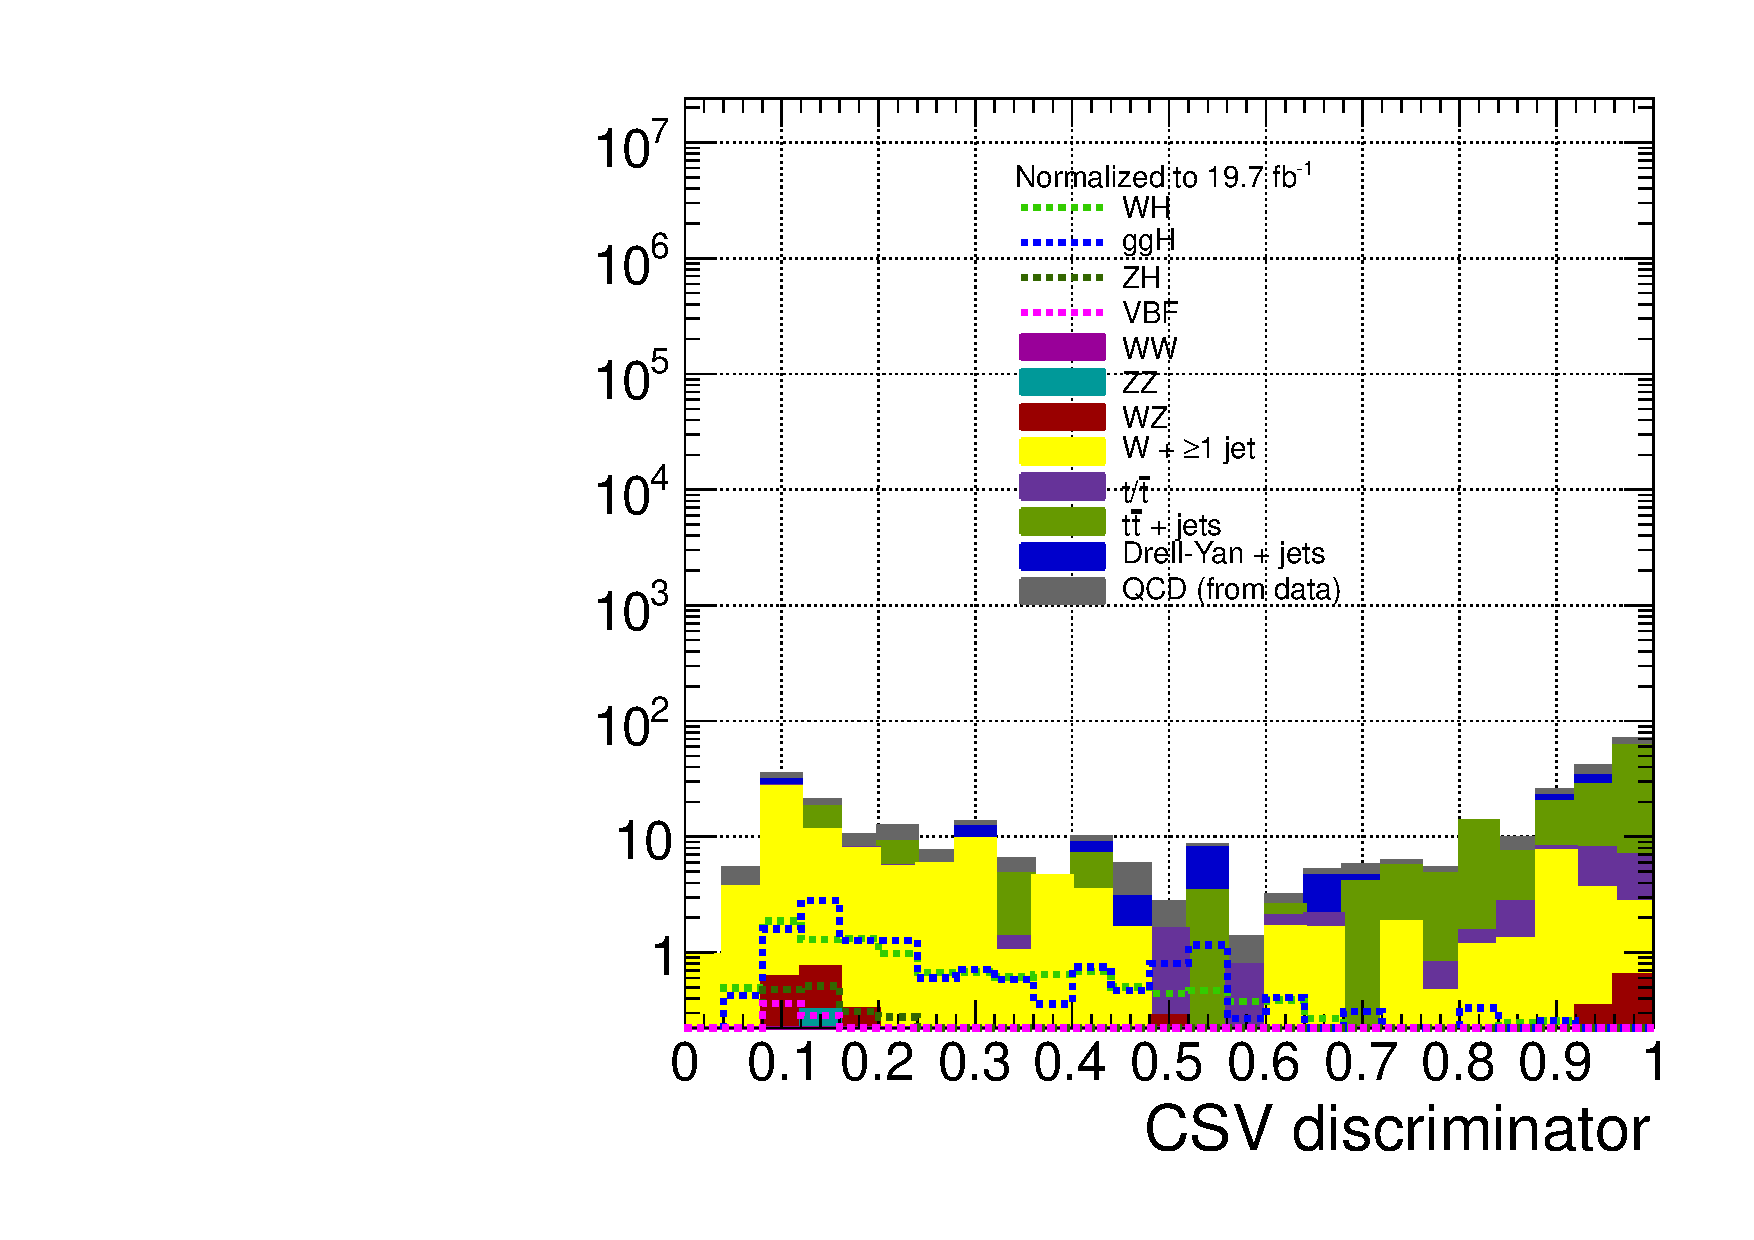
\includegraphics[width=\cmsFigWidth]{figures/sigVsBkg_csv_regA_highMT_v61}
    \caption{Distribution of the CSV discriminator for four signal models and all backgrounds, including data-driven QCD, after all the preselection cuts except the b veto have been applied. Normalized to 19.7 \fbinv. (\cmsLeft) Low-$M_{\text{T}}$ bin. (\cmsRight) High-$M_{\text{T}}$ bin.}
    \label{fig:sigVsBkg_csv_regA}
  \end{center}
\end{figure}

As shown in Figure~\ref{fig:sigVsBkg_csv_regA}, the distribution of the CSV discriminator for signal events tends to peak at low values of the discriminator, while single top and $t\bar{t}$ events with real b-jets peak at high values; thus, since no data/MC b-veto efficiency scale factors exist for tau jets, we make the approximation that the tau jets in our signal behave more like light jets with regard to the CSV discriminator, and so the expected signal is corrected for differences between data and MC b-veto efficiency using the BTV-provided scale factors~\cite{CMS:btaguncertaintytwiki} for light jets.  The scale factors are binned in HPS tau parent (cleaned) jet $\eta$ and $p_T$.

\begin{figure}[hbtp]
  \begin{center}
    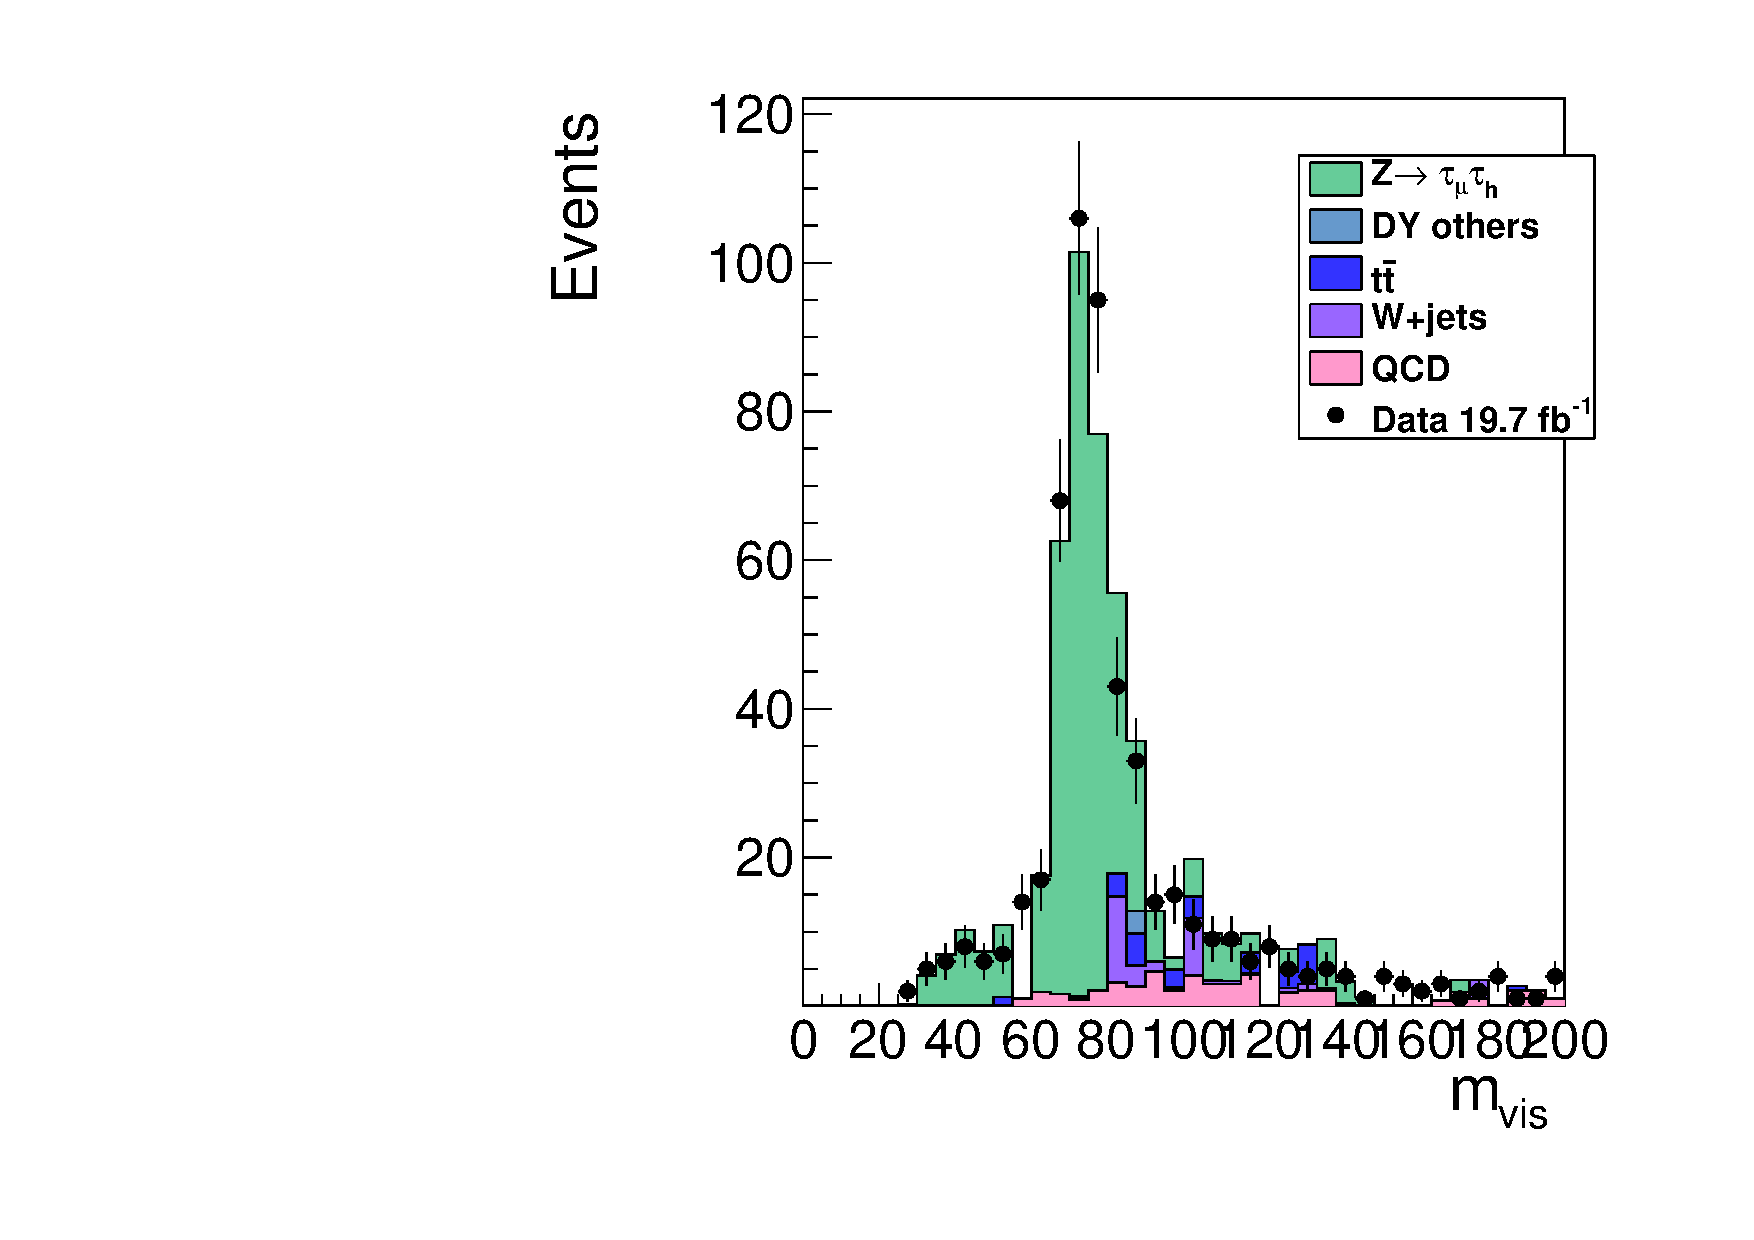
\includegraphics[width=\cmsFigWidth]{figures/PassNN_mvis}
    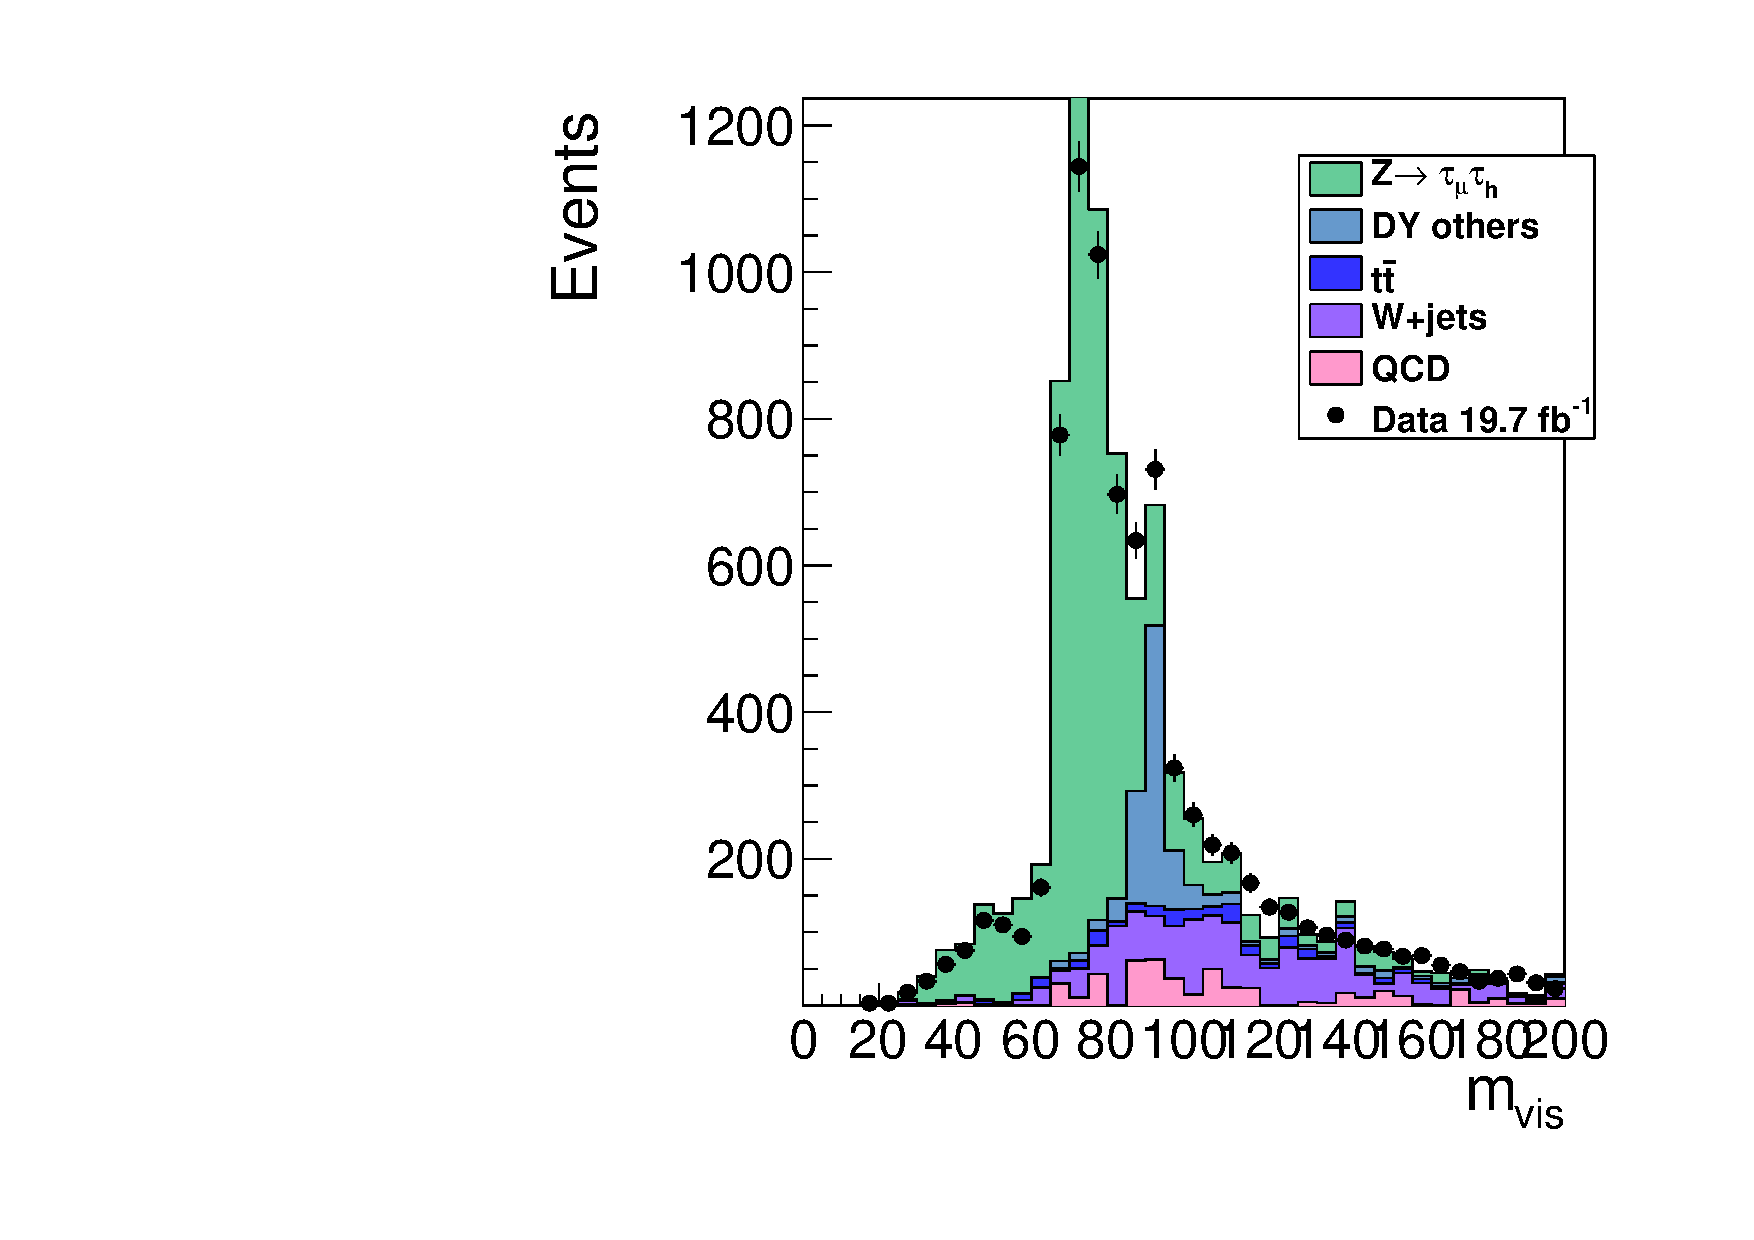
\includegraphics[width=\cmsFigWidth]{figures/FailNN_mvis}
    \caption{$\tau_{\mu}\tau_{\text{had}}$ invariant mass plots showing Z peak in Run I data and MC, for events passing all Z peak selections including the medium combined isolation discriminator for $\tau_{\text{had}}$, and passing or failing the medium CSV b-tag applied to the jet that seeded the $\tau_{\text{had}}$. (\cmsLeft) Events passing the medium CSV b-tag. (\cmsRight) Events failing the medium CSV b-tag.}
    \label{fig:BTagZPeakPassFail}
  \end{center}
\end{figure}

Two methods are used to assess the error on the expected signal due to the uncertainty on the scale factors. Firstly, the expected signal is recalculated for a coherent +1$\sigma$ shift in the scale factors in all simulated events, and then again for a -1$\sigma$ shift; the difference between the nominal and $\pm1\sigma$-shifted expected signal is taken as the $\pm1\sigma$ error due to b-tag scale factors for light jets. Secondly, another systematic is calculated to account for the uncertainty of using light-jet scale factors for tau jets; the signal yields after the final selection are calculated using light-jet scale factors (the nominal method) and using b-jet scale factors (the logic being that the phase space for tau jets should be somewhere between the two extremes of light jets and b jets), and the percent difference in the yield is taken as a conservative uncertainty on the yield due to the usage of light-jet scale factors.

Since a b-veto is applied to a tau jet, the following cross-check has been performed to verify that the assigned systematic uncertainty for a potential data/MC discrepancy is adequate. First, a clean sample of of tau lepton candidates was obtained using $Z\rightarrow\tau_{\mu}\tau_{\text{had}}$ selections in Run I data and MC and the Z peak was reconstructed as per the methods in~\cite{Tau14001}, requiring that the $\tau_{\text{had}}$ object pass the medium combined isolation discriminator. Then, additionally, a b-tag at the medium CSV working point was applied to the jets that seeded the $\tau_{\text{had}}$, and two Z peaks were plotted -- one for events passing the b-tag and one for events failing the b-tag. The Z peak plots are shown in Figure~\ref{fig:BTagZPeakPassFail}; these results suggest that the data/MC agreement is unaffected by whether the tau jets pass or fail the CSV b-tag, and also it can be seen that the percentage of events in data and MC that pass the medium CSV b-tag is in the neighbourhood of 10\%, which is similar to the proportion of signal MC events observed to pass the medium CSV b-tag. Thus, these results lend confidence to the assumption that the requirement for the tau jet to pass the medium CSV b-veto does not significantly affect the known data/MC discrepancy covered by the present systematic uncertainty.

%PV
\section{Primary vertex compatibility requirement\label{sec:evtsel-dz}}
To reduce the background from $\tau_{\mu}\tau_{\text{had}}$ pairs in which the $\tau_{\mu}$ and $\tau_{\text{had}}$ come from different $pp$ interactions, we require $d_{\text{z}}(\tau_{\mu},\text{PV}) <$ 0.5 \cm and $d_{\text{z}}(\tau_{\text{had}},\text{PV}) <$ 0.2 cm, where PV refers to the hardest (primary) interaction in the event.  These cuts are recommended by the MUO and TAU POGs.  The $d_{\text{z}}(\tau_{\mu},\text{PV})$ and $d_{\text{z}}(\tau_{\text{had}},\text{PV})$ distributions for events passing all preselection cuts except those plotted are shown in Figures~\ref{fig:sigVsBkg_dz_regA_lowMT} and~\ref{fig:sigVsBkg_dz_regA_highMT}.

\begin{figure}[hbtp]
  \begin{center}
    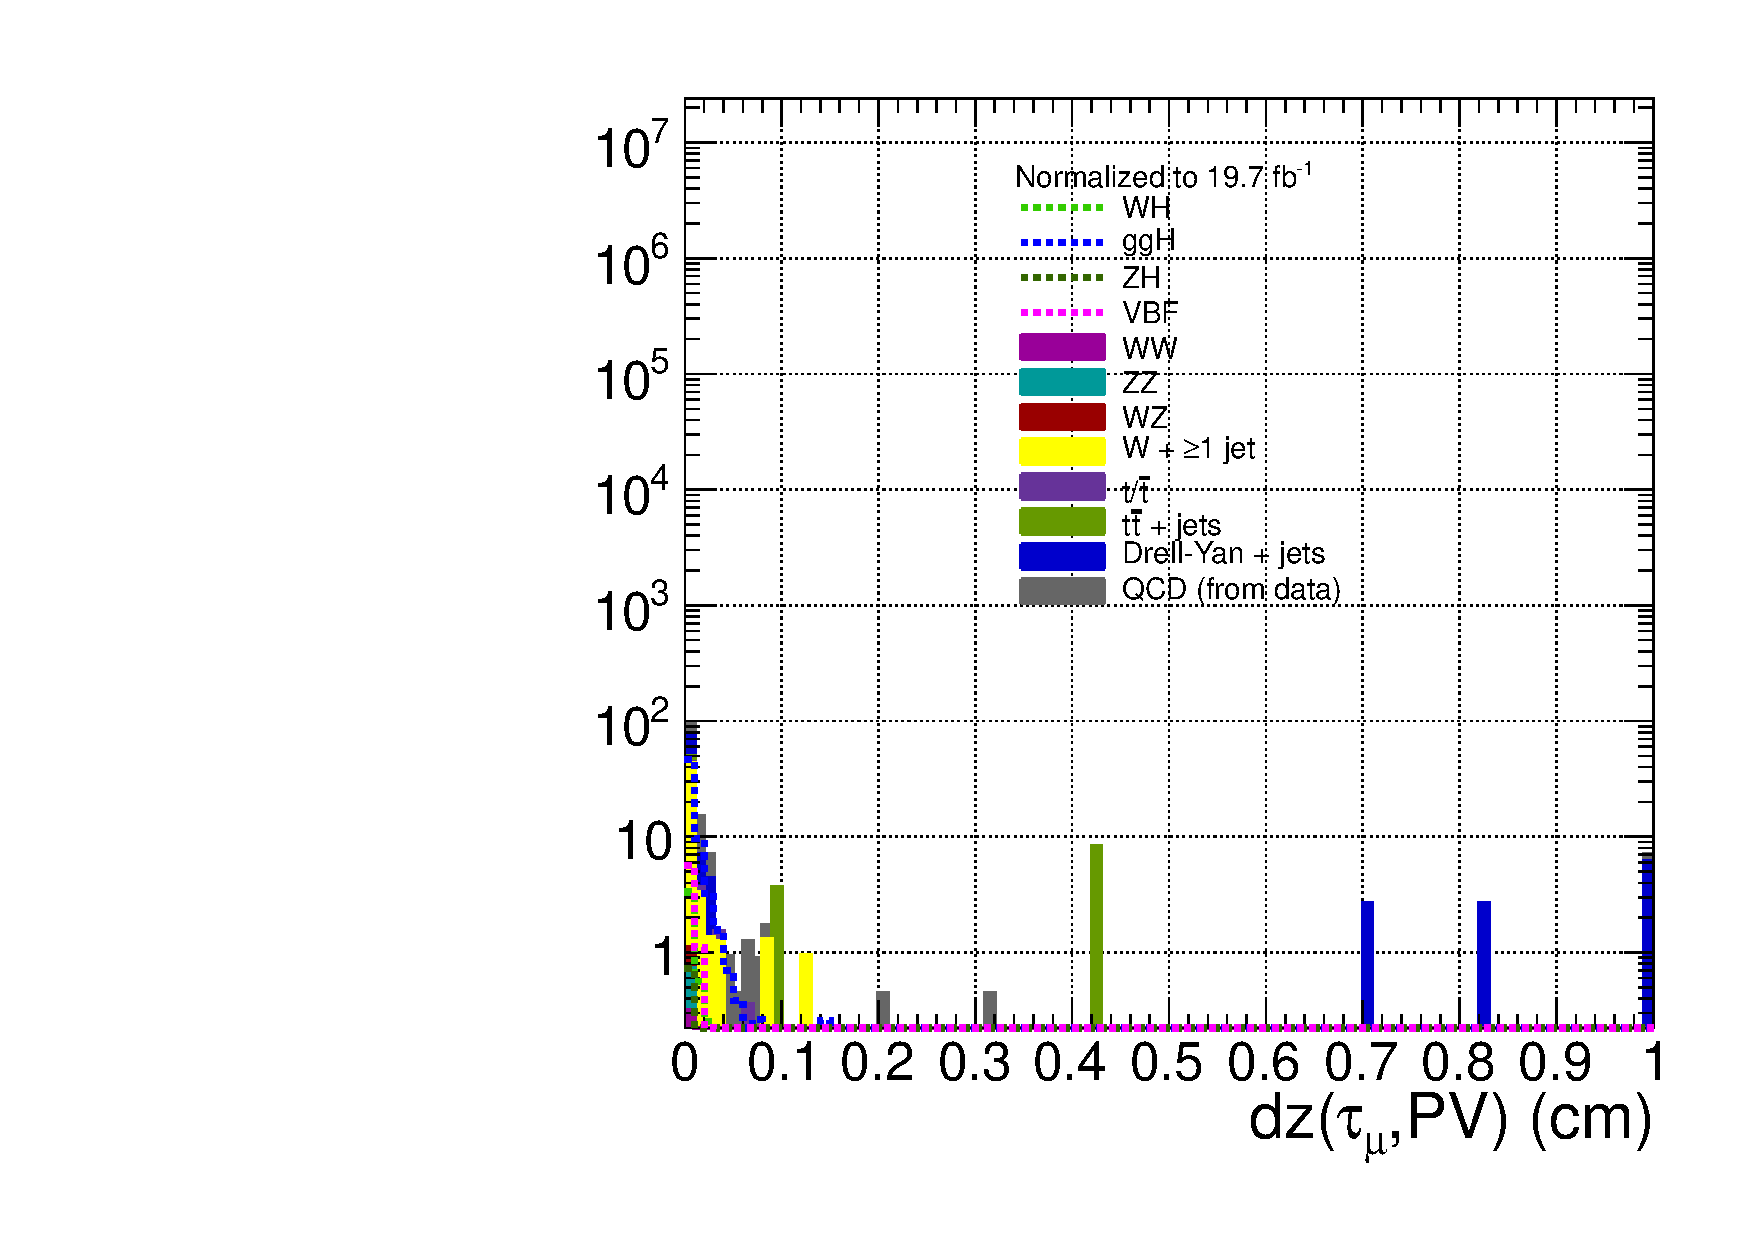
\includegraphics[width=1.2\cmsFigWidth]{figures/sigVsBkg_dztaumu_regA_lowMT_v60}
    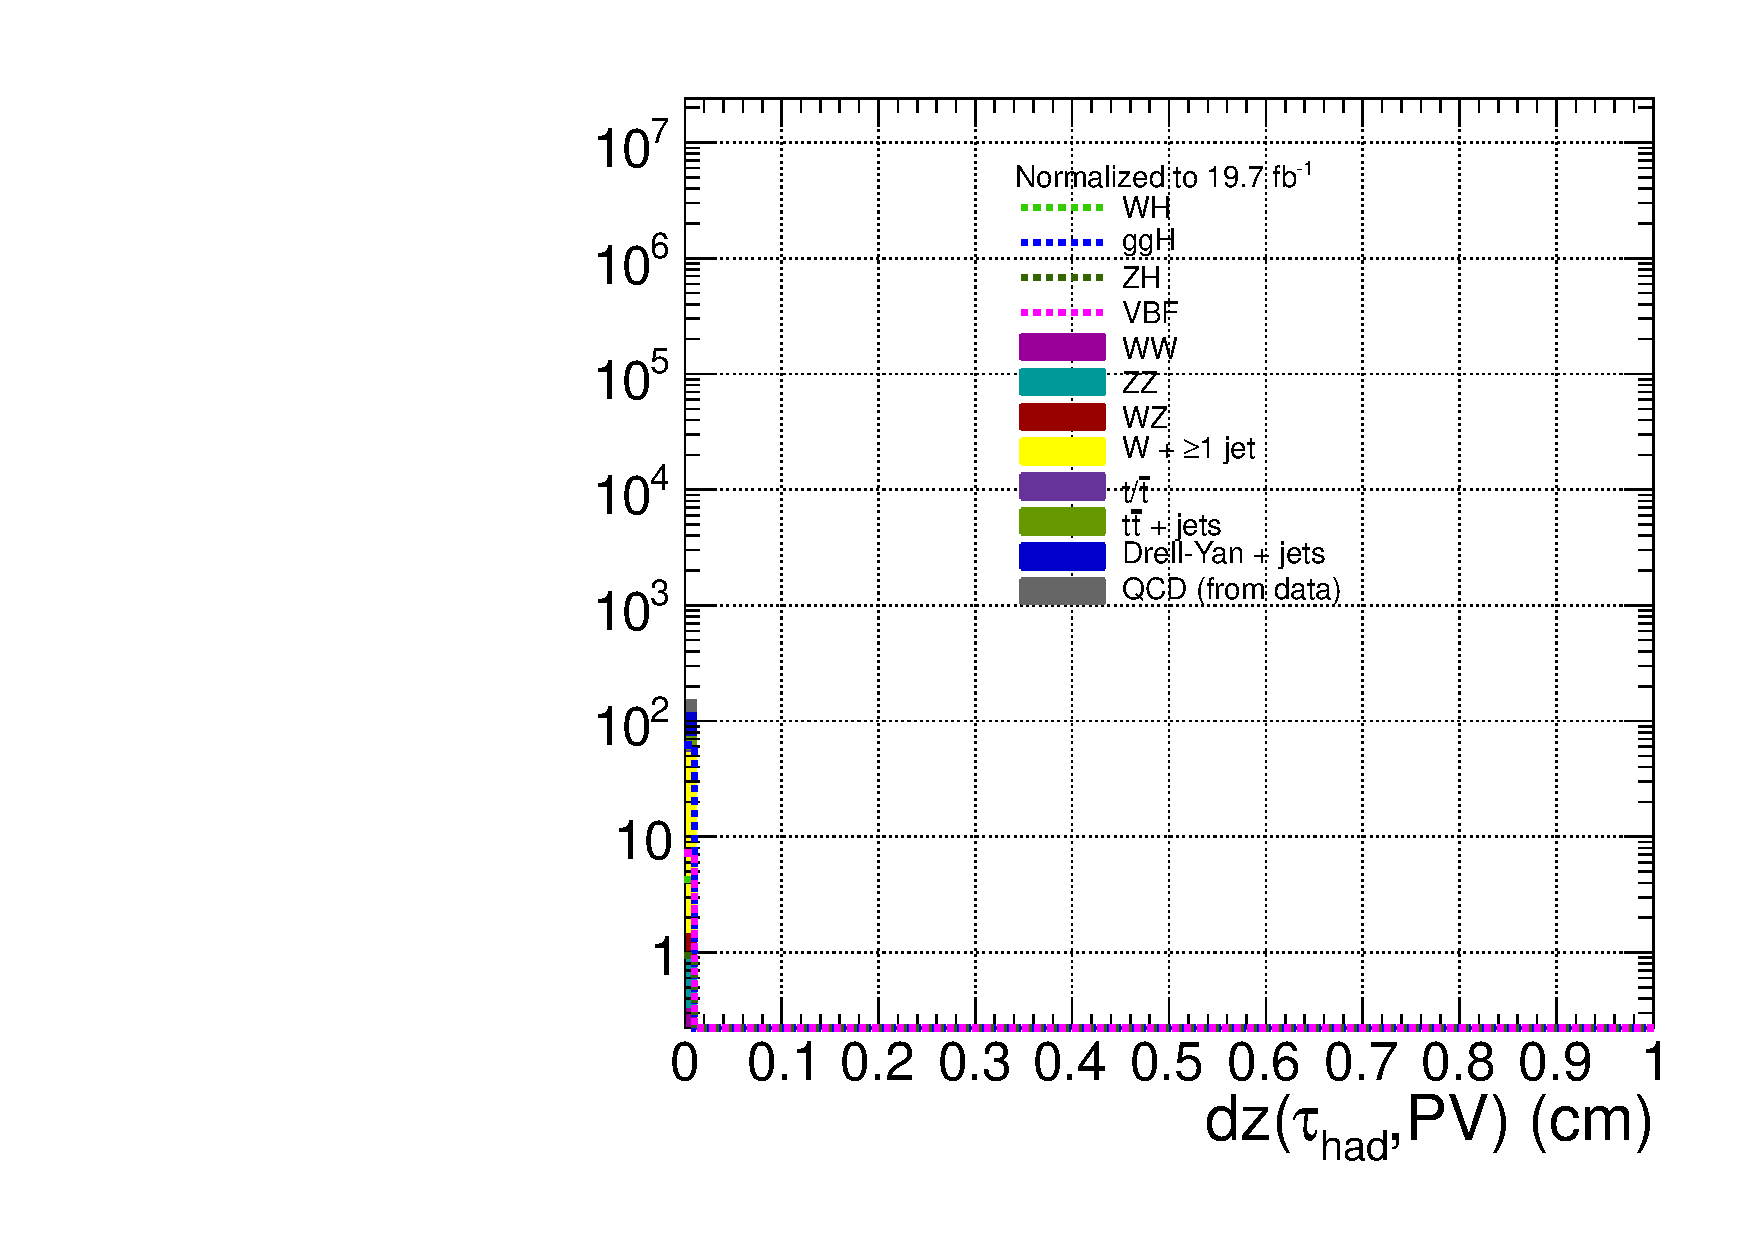
\includegraphics[width=1.2\cmsFigWidth]{figures/sigVsBkg_dztauhad_regA_lowMT_v60}
    \caption{Distribution of (\cmsLeft) dz($\tau_{\mu}$,PV) and (\cmsRight) dz($\tau_{\text{had}}$,PV) in the low-$M_{T}$ bin for four signal models and all backgrounds including data-driven QCD, after all the preselection cuts except the dz cuts have been applied. Normalized to 19.7 \fbinv.}
    \label{fig:sigVsBkg_dz_regA_lowMT}
  \end{center}
\end{figure}

\begin{figure}[hbtp]
  \begin{center}
    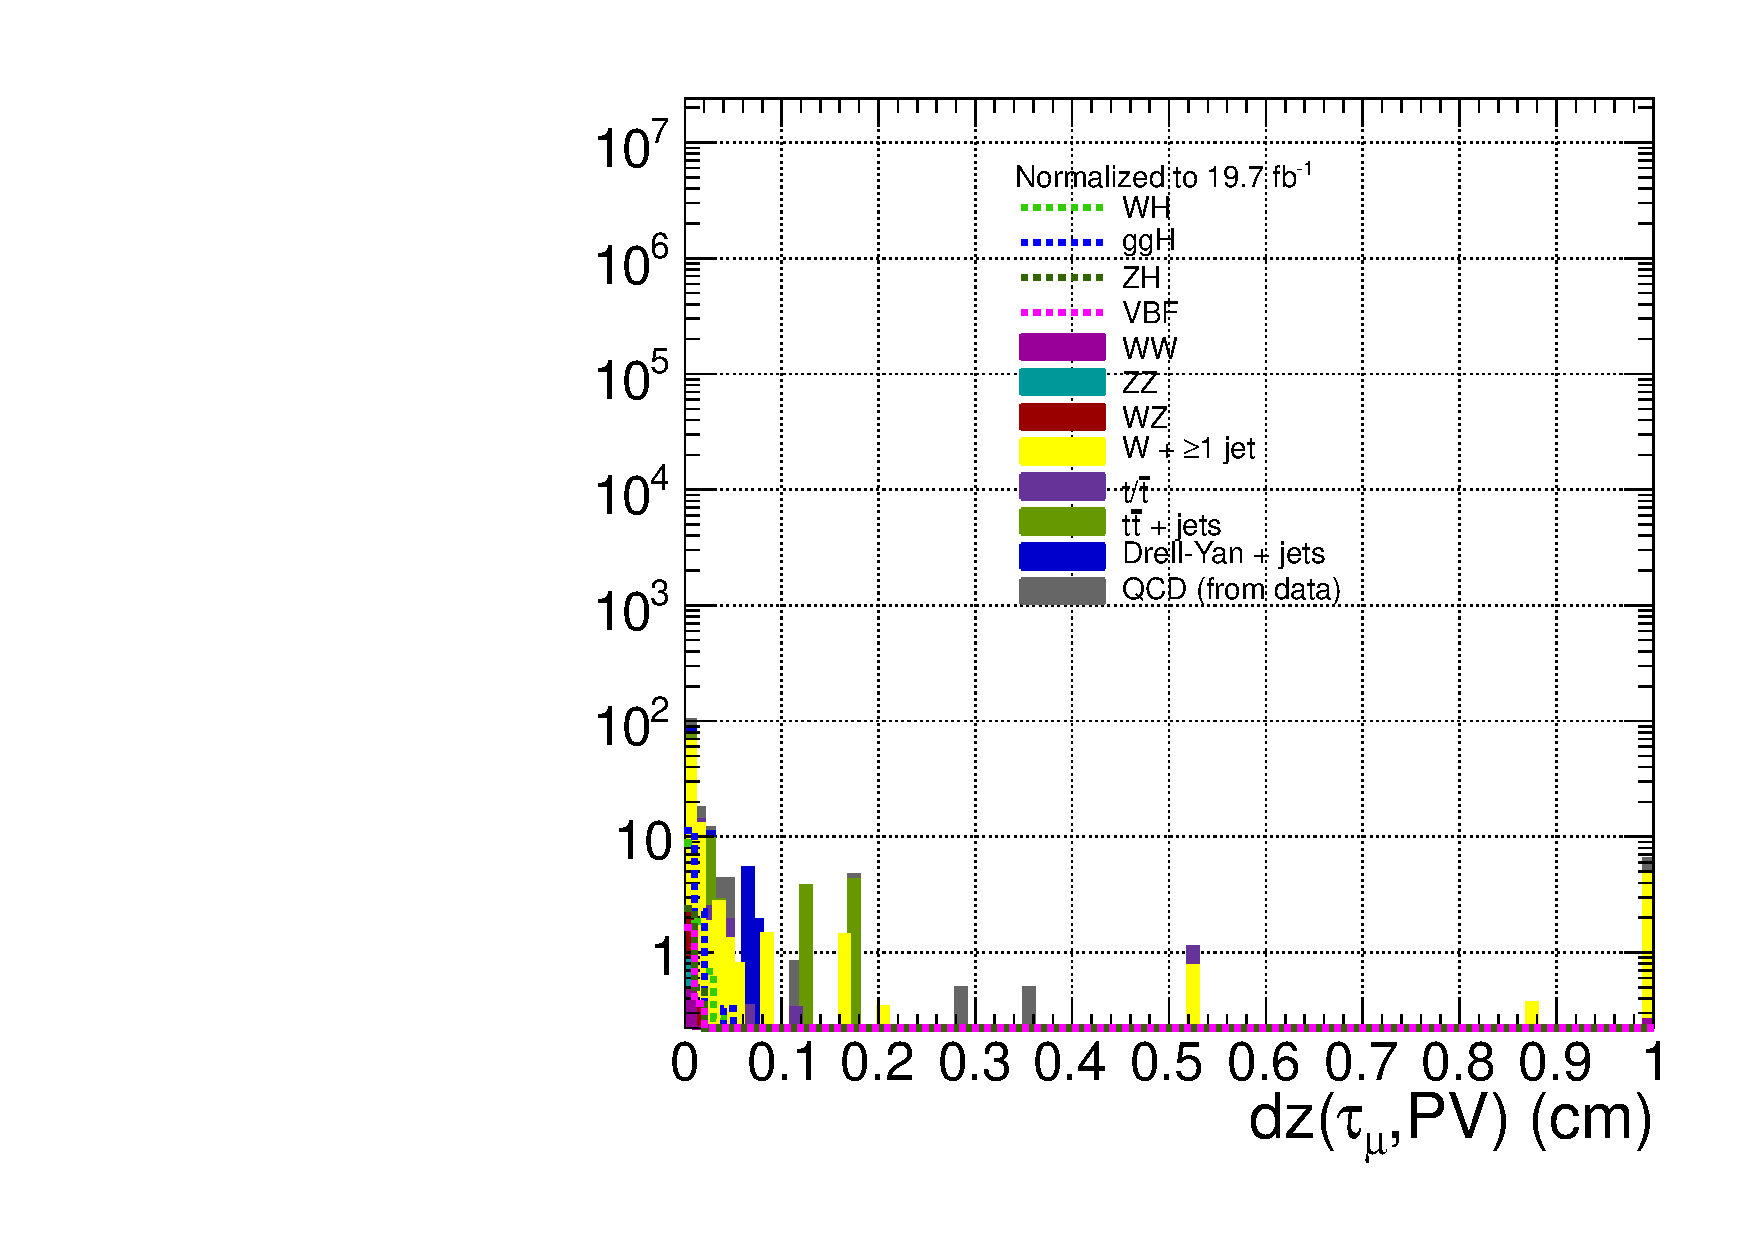
\includegraphics[width=1.2\cmsFigWidth]{figures/sigVsBkg_dztaumu_regA_highMT_v60}
    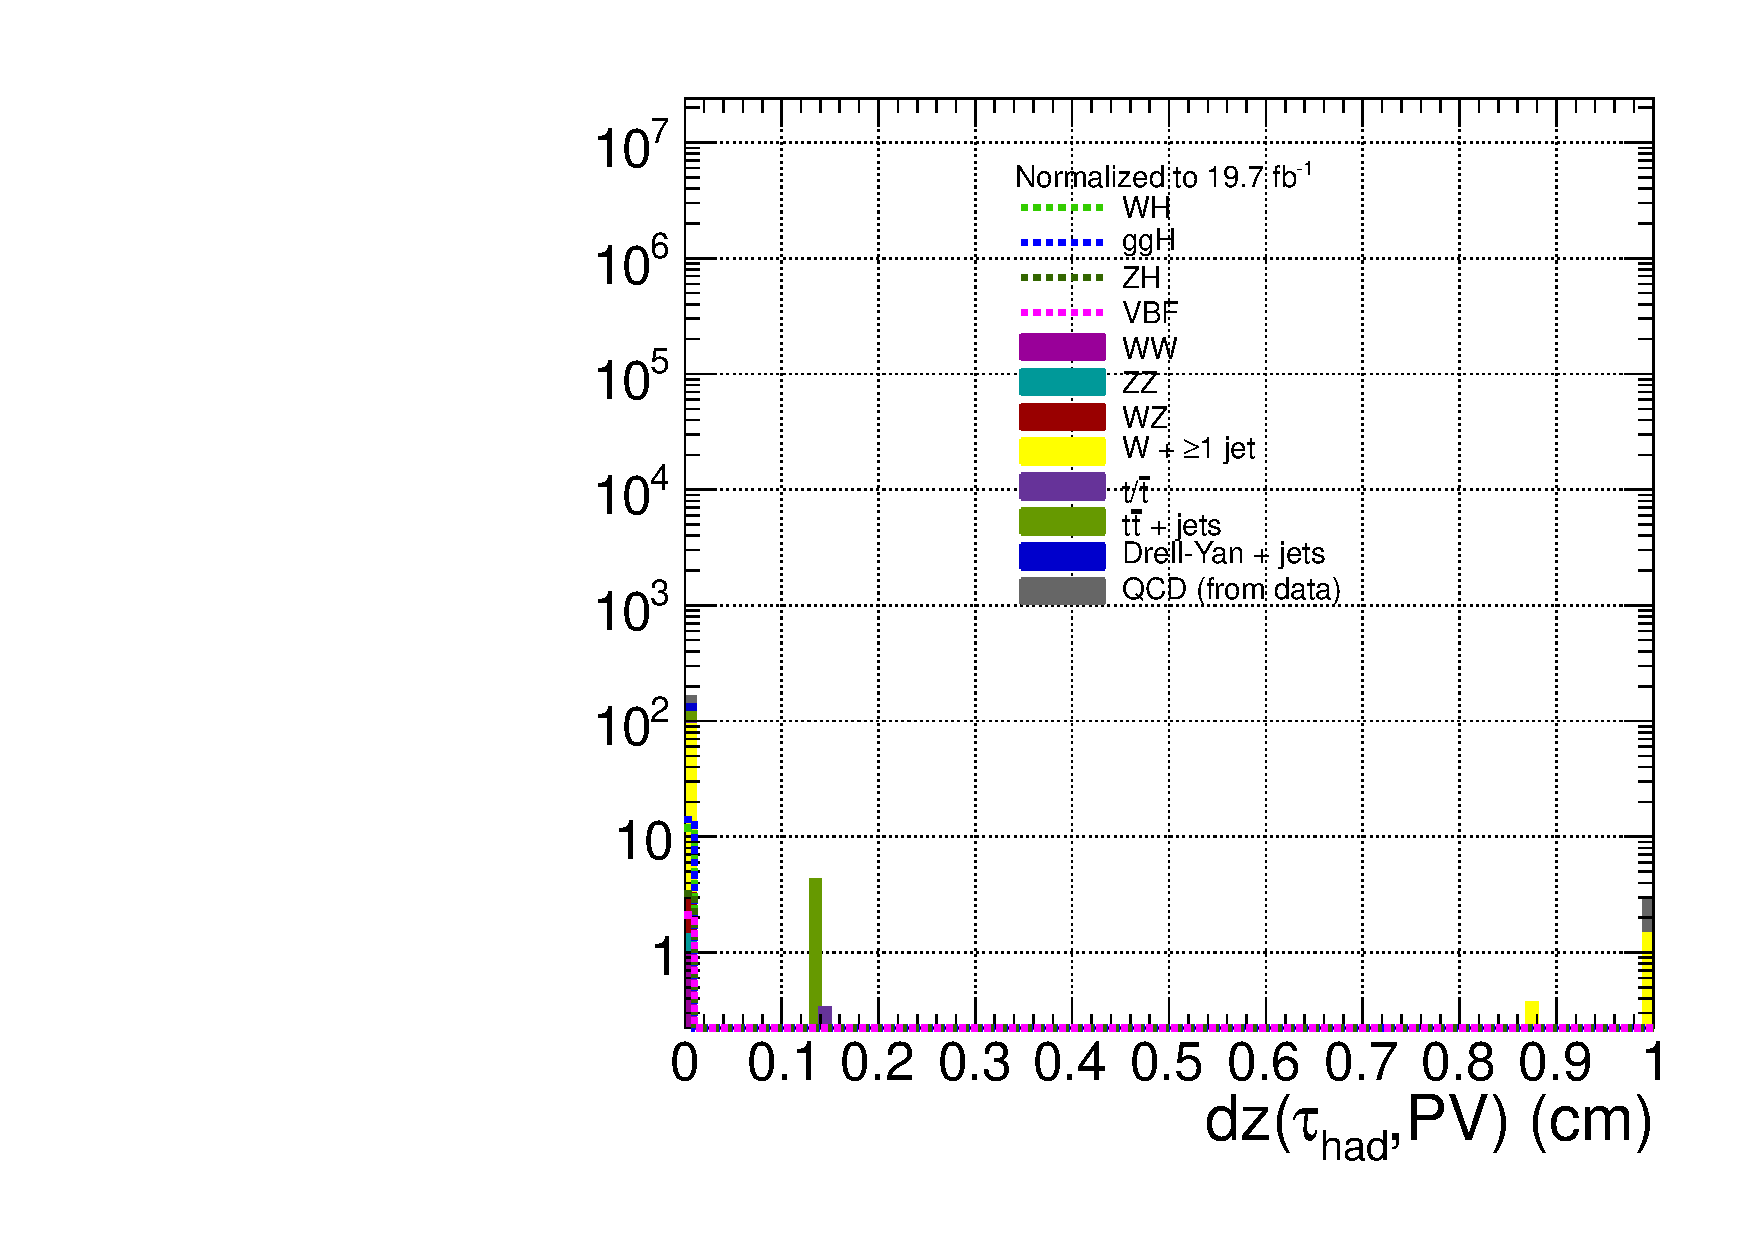
\includegraphics[width=1.2\cmsFigWidth]{figures/sigVsBkg_dztauhad_regA_highMT_v60}
    \caption{Distribution of (\cmsLeft) dz($\tau_{\mu}$,PV) and (\cmsRight) dz($\tau_{\text{had}}$,PV) in the high-$M_{T}$ bin for four signal models and all backgrounds including data-driven QCD, after all the preselection cuts except the dz cuts have been applied. Normalized to 19.7 \fbinv.}
    \label{fig:sigVsBkg_dz_regA_highMT}
  \end{center}
\end{figure}

%MT
\section{Transverse mass regions \label{sec:evtsel-mt}}

Figure~\ref{fig:sigVsBkg_MET_MT_regA} shows the $M_{\text{T}}$ distribution for four signal models and all backgrounds.  The gluon fusion signal is clustered at low $M_{\text{T}}$, where Drell-Yan and QCD are the most important backgrounds.  The WH signal can be found in the high $M_{\text{T}}$ bin, where $W$+jets and $t\bar{t}$ dominate the background.  We define $M_{\text{T}} \le$ 50 GeV as the low-$M_{\text{T}}$ bin of this search, sensitive to ggH and VBF, and $M_{\text{T}} >$ 50 GeV as the high-$M_{\text{T}}$ bin, sensitive to WH.  The cut was chosen to optimize S/$\sqrt{\text{S} + \text{B}}$ for the WH signal in the high-$M_{\text{T}}$ bin.  The $M_{\text{T}}$ in this search is calculated using Type I-corrected~\cite{1748-0221-6-11-P11002} PAT \ETslash, which is also used in the calculation of \ETslash systematics~\cite{METuncertainty}.

\begin{figure}[hbtp]
  \begin{center}
    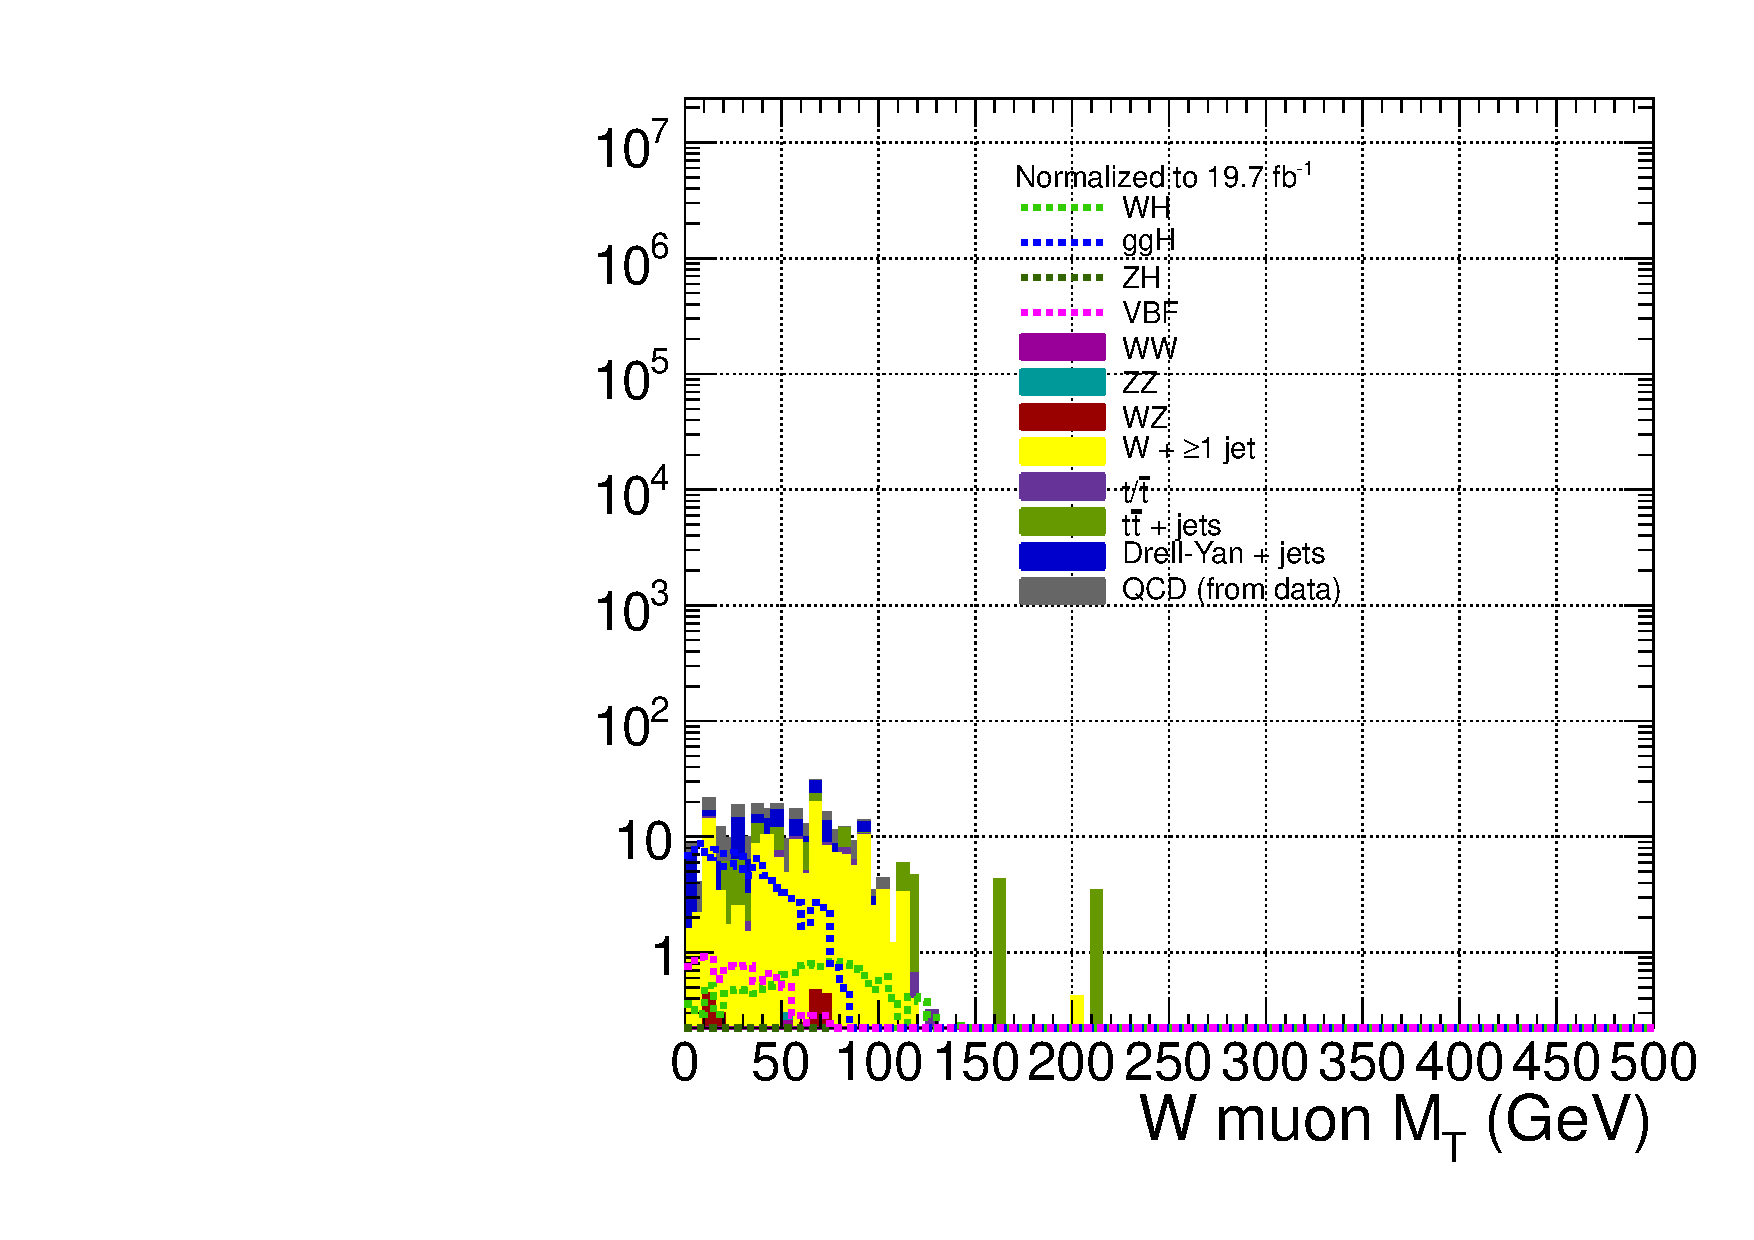
\includegraphics[width=1.2\cmsFigWidth]{figures/sigVsBkg_MT_regA_v62}
    \caption{$M_{\text{T}}$ distribution after the preselection (excluding the $M_{\text{T}}$ cut) has been applied for four signal models and all backgrounds. The term ``$W$ muon'' in the label refers to the trigger muon, not necessarily a muon from a $W$ decay (as in the case of the ggH signal, for instance).}
    \label{fig:sigVsBkg_MET_MT_regA}
  \end{center}
\end{figure}

Following the JME approved procedure~\cite{METuncertainty}, uncertainty on the expected signal in each $M_{\text{T}}$ bin due to \ETslash scale is assessed by independently varying the e/$\gamma$, muon, tau, jet, and unclustered energy scales up and down by their approved 1$\sigma$ errors for each event in the signal sample.  \ETslash and $M_{\text{T}}$ are recalculated in each event, yielding an expected signal estimate in each of the +1$\sigma$ and -1$\sigma$ scenarios.  For each energy scale variation, the larger of the $\pm1\sigma$ deviations from nominal is taken as the error due to the uncertainty on that energy scale.  The quadrature sum of these individual errors is taken as the total $\pm1\sigma$ error due to \ETslash scale.

For technical reasons, the \ETslash definition for the $\pm1\sigma$ varied \ETslash collections and the nominal from which deviations are measured is slightly different from the \ETslash definition used when quoting the expected signal.  However, the deviations for the \ETslash uncertainty calculation are measured in a consistent way (same \ETslash definition for varied and nominal collections), and it is only the percent difference which is quoted as the \ETslash scale error.

%Final selection
\section{Search region \label{sec:evtsel-search}}
Table~\ref{tab:cut-flow-MC} shows the number of events surviving each successive cut in the selection sequence for the $m_a$ = 9 GeV WH and ggH signal samples and all background Monte Carlo samples (except for QCD Monte Carlo, due to poor statistics) used in the selection sequence optimization.  Table~\ref{tab:cut-flow-WHSignal} displays the selection efficiencies for the WH signal samples for each selection cut, expressed as the fraction of triggered signal events (i.e., events passing the HLT) surviving after each cut.  Table~\ref{tab:cut-flow-ggHSignal} shows the analogous selection efficiencies for the ggH signal samples.  The number of events is scaled to 19.7 fb$^{-1}$ using the cross sections given in Tables~\ref{tab:MCBkg} and~\ref{tab:MC-sig}.

%\begin{table*}[htbh]
\begin{sidewaystable}
\begin{center}
\caption{Number of events in MC signal and background datasets remaining after each cut in the selection sequence.  The signal samples have a pseudoscalar mass of 9 GeV.  The number of events is scaled to 19.7 \fbinv using the cross sections given in Tables~\ref{tab:MCBkg} and~\ref{tab:MC-sig}.  For the rows labeled ``$d_{\text{Z}}$ to PV'' and ``$m_{\mu+\text{had}} >$ 4 GeV'', pileup reweighting has been applied, while for the other rows, no pileup reweighting has been applied.\label{tab:cut-flow-MC}}
\resizebox{\columnwidth}{!}{
\begin{tabular}{|m{2.5cm}|c|c|c|c|c|c|c|c|c|c|c|}
  \hline
  \multicolumn{2}{|l|}{Cut} & WH & ggH & W+$\ge$1 jet & Drell-Yan + jets & $t\bar{t}$ + jets & Single top & WZ & ZZ & WW \\
  \hline
  \hline
  \multicolumn{2}{|l|}{} & 4.522\ten{3} & 6.721\ten{4} & 1.883\ten{8} & 3.587\ten{8} & 4.842\ten{6} & 1.825\ten{6} & 6.542\ten{5} & 3.478\ten{5} & 1.080\ten{6} \\
  \hline
  \multicolumn{2}{|l|}{\texttt{HLT\_IsoMu24\_eta2p1}} & 1.024\ten{3} & 6.616\ten{3} & 2.723\ten{7} & 1.507\ten{7} & 6.359\ten{5} & 1.124\ten{5} & 5.203\ten{4} & 1.937\ten{4} & 1.167\ten{5} \\
  \hline
  \multicolumn{2}{|l|}{Trigger $\mu p_T$} & 1.001\ten{3} & 6.083\ten{3} & 2.633\ten{7} & 1.459\ten{7} & 6.238\ten{5} & 1.091\ten{5} & 5.090\ten{4} & 1.913\ten{4} & 1.138\ten{5} \\
  \hline
  \multicolumn{2}{|l|}{Trigger $\mu \eta$, ID, and isolation} & 9.065\ten{2} & 4.417\ten{3} & 2.410\ten{7} & 1.381\ten{7} & 5.543\ten{5} & 9.936\ten{4} & 4.732\ten{4} & 1.816\ten{4} & 1.043\ten{5} \\
  \hline
  \multicolumn{2}{|l|}{$\tau_{\mu} p_T$, $\eta$, and ID} & 2.702\ten{2} & 2.600\ten{3} & 2.950\ten{5} & 3.705\ten{6} & 1.449\ten{5} & 1.430\ten{4} & 7.300\ten{3} & 6.842\ten{3} & 6.138\ten{3} \\
  \hline
  \multicolumn{2}{|l|}{HPS $\eta$ and ID} & 1.270\ten{2} & 9.838\ten{2} & 7.518\ten{4} & 9.074\ten{4} & 6.805\ten{4} & 6.508\ten{3} & 7.541\ten{2} & 6.257\ten{2} & 7.861\ten{2} \\
  \hline
  \multicolumn{2}{|l|}{HPS $p_T$ and isolation}                          & 39.06 & 216.0 & 1145  & 4338   & 798.3 & 85.56  & 24.53  & 24.35  & 13.18 \\
  \hline
  \multicolumn{2}{|l|}{b-veto}                              & 34.28 & 194.8 & 903.6 & 4170   & 273.2 & 20.40  & 20.41  & 21.93  & 10.26 \\
  \hline
  \multicolumn{2}{|l|}{HLT matching}                                   & 33.99 & 194.0 & 903.6 & 4088   & 266.1 & 20.40  & 19.95  & 21.33  & 10.05 \\
  \hline
  \multicolumn{2}{|l|}{$q(\tau_{\mu}) \times q(\text{trigger }\mu)$} & 16.70 & 92.56 & 171.0 & 93.21  & 81.60 & 8.365  & 3.075  & 1.455  & 1.404 \\
  \hline
  \multicolumn{2}{|l|}{$q(\tau_{\mu}) \times q(\tau_{\text{had}})$}     & 16.55 & 91.80 & 154.3 & 68.84  & 67.41 & 6.901  & 2.159  & 1.171  & 1.296 \\
  \hline
  \multicolumn{2}{|l|}{Trigger $\mu$ nearby lepton filter}       & 16.37 & 79.80 & 153.1 & 68.84  & 63.86 & 6.901  & 2.159  & 1.171  & 1.296 \\
  \hline
  \hline
  \multicolumn{2}{|l|}{\textbf{$M_{\text{T}} >$ 50 GeV}}              & 12.04 & 14.91 & 95.40 & 22.66  & 39.03 & 5.389  & 1.701  & 0.4968 & 0.8642 \\
  \hline
  \multicolumn{2}{|r|}{$d_{\text{Z}}$ to PV}                           & 11.77 & 13.52 & 84.15 & 20.85  & 25.10 & 4.306  & 1.783  & 0.4766 & 0.7122 \\
  \hline
  \multicolumn{2}{|r|}{$m_{\mu+\text{had}} >$ 4 GeV} & 6.972 & 7.598 & 1.761 & 0.4630 & 0     & 0      & 0.4038 & 0.1447 & 0 \\
  \hline
  \hline
  \multicolumn{2}{|l|}{\textbf{$M_{\text{T}} \le$ 50 GeV}}            & 4.326 & 64.89 & 57.67 & 46.18  & 24.84 & 1.512  & 0.4580 & 0.6743 & 0.4321 \\
  \hline
  \multicolumn{2}{|r|}{$d_{\text{Z}}$ to PV}                           & 4.225 & 60.79 & 50.30 & 32.03  & 17.62 & 1.839  & 0.5187 & 0.5394 & 0.3159 \\
  \hline
  \multicolumn{2}{|r|}{$m_{\mu+\text{had}} >$ 4 GeV} & 2.723 & 46.35 & 0     & 5.248  & 4.104 & 0.2781 & 0      & 0.1082 & 0 \\
  \hline
\end{tabular}
}
\end{center}
\end{sidewaystable}

\begin{sidewaystable}
\begin{center}
\caption{Selection efficiencies for MC WH signal samples, expressed as the fraction of triggered events surviving each selection cut.\label{tab:cut-flow-WHSignal}}
\resizebox{\columnwidth}{!}{
\begin{tabular}{|m{2.5cm}|c|c|c|c|c|c|c|}
  \hline
  \multicolumn{2}{|l|}{Cut} & $m_a$ = 5 GeV & $m_a$ = 7 GeV & $m_a$ = 9 GeV & $m_a$ = 11 GeV & $m_a$ = 13 GeV & $m_a$ = 15 GeV \\
  \hline
  \hline
  \multicolumn{2}{|l|}{Trigger $\mu p_T$} & 0.9780 & 0.9779 & 0.9769 & 0.9765 & 0.9754 & 0.9739 \\
  \hline
  \multicolumn{2}{|l|}{Trigger $\mu \eta$, ID, and isolation} & 0.8841 & 0.8841 & 0.8850 & 0.8801 & 0.8795 & 0.8802 \\
  \hline
  \multicolumn{2}{|l|}{$\tau_{\mu} p_T$, $\eta$, and ID} & 0.2898 & 0.2814 & 0.2638 & 0.2643 & 0.2620 & 0.2570 \\
  \hline
  \multicolumn{2}{|l|}{HPS $\eta$ and ID} & 0.1688 & 0.1476 & 0.1240 & 0.1189 & 0.1051 & 0.0914 \\
  \hline
  \multicolumn{2}{|l|}{HPS $p_T$ and isolation} & 0.0485 & 0.0439 & 0.0381 & 0.0379 & 0.0338 & 0.0282 \\
  \hline
  \multicolumn{2}{|l|}{b-veto} & 0.0407 & 0.0382 & 0.0335 & 0.0334 & 0.0305 & 0.0256 \\
  \hline
  \multicolumn{2}{|l|}{HLT matching} & 0.0404 & 0.0380 & 0.0332 & 0.0332 & 0.0303 & 0.0254 \\
  \hline
  \multicolumn{2}{|l|}{$q(\tau_{\mu}) \times q(\text{trigger }\mu)$} & 0.0204 & 0.0192 & 0.0163 & 0.0167 &  0.0152 & 0.0125 \\
  \hline
  \multicolumn{2}{|l|}{$q(\tau_{\mu}) \times q(\tau_{\text{had}})$} & 0.0202 & 0.0190 & 0.0162 & 0.0166 & 0.0150 & 0.0124 \\
  \hline
  \multicolumn{2}{|l|}{Trigger $\mu$ nearby lepton filter} & 0.0200 & 0.0188 & 0.0160 & 0.0165 & 0.0148 & 0.0124 \\
  \hline
  \multirow{2}{*}{\textbf{$M_{\text{T}} \le$  50 GeV}} & $d_{\text{Z}}$ to PV & 0.00575 & 0.00494 & 0.00413 & 0.00480 & 0.00364 & 0.00342 \\
  & $m_{\mu+\text{had}} >$ 4 GeV & 0.00114 & 0.00148 & 0.00266 & 0.00403 & 0.00329 & 0.00335 \\
  \hline
  \multirow{2}{*}{\textbf{$M_{\text{T}} >$  50 GeV}} & $d_{\text{Z}}$ to PV & 0.0140 & 0.0136 & 0.0115 & 0.0111 & 0.0106 & 0.00835 \\
  & $m_{\mu+\text{had}} >$ 4 GeV & 0.000101 & 0.00379 & 0.00681 & 0.00837 & 0.00932 & 0.00774 \\
  \hline
\end{tabular}
}
\end{center}
\end{sidewaystable}

\begin{sidewaystable}
\begin{center}
\caption{Selection efficiencies for MC ggH signal samples, expressed as the fraction of triggered events surviving each selection cut.\label{tab:cut-flow-ggHSignal}}
\resizebox{\columnwidth}{!}{
\begin{tabular}{|m{2.5cm}|c|c|c|c|c|c|c|}
  \hline
  \multicolumn{2}{|l|}{Cut} & $m_a$ = 5 GeV & $m_a$ = 7 GeV & $m_a$ = 9 GeV & $m_a$ = 11 GeV & $m_a$ = 13 GeV & $m_a$ = 15 GeV \\
  \hline
  \hline
  \multicolumn{2}{|l|}{Trigger $\mu p_T$} & 0.9147 & 0.9226 & 0.9194 & 0.9169 & 0.9156 & 0.9155 \\
  \hline
  \multicolumn{2}{|l|}{Trigger $\mu \eta$, ID, and isolation} & 0.6093 & 0.6491 & 0.6675 & 0.6979 & 0.7328 & 0.7623 \\
  \hline
  \multicolumn{2}{|l|}{$\tau_{\mu} p_T$, $\eta$, and ID} & 0.4308 & 0.4082 & 0.3931 & 0.3973 & 0.4091 & 0.4173 \\
  \hline
  \multicolumn{2}{|l|}{HPS $\eta$ and ID} & 0.1846 & 0.1679 & 0.1487 & 0.1319 & 0.1151 & 0.0918 \\
  \hline
  \multicolumn{2}{|l|}{HPS $p_T$ and isolation} & 0.0364 & 0.0345 & 0.0327 & 0.0302 & 0.0250 & 0.0166 \\
  \hline
  \multicolumn{2}{|l|}{b-veto} & 0.0321 & 0.0303 & 0.0294 & 0.0280 & 0.0232 & 0.0153 \\
  \hline
  \multicolumn{2}{|l|}{HLT matching} & 0.0316 & 0.0301 & 0.0293 & 0.0279 & 0.0230 & 0.0152 \\
  \hline
  \multicolumn{2}{|l|}{$q(\tau_{\mu}) \times q(\text{trigger }\mu)$} & 0.0154 & 0.0144 & 0.0140 & 0.0133 & 0.0117 & 0.0073 \\
  \hline
  \multicolumn{2}{|l|}{$q(\tau_{\mu}) \times q(\tau_{\text{had}})$} & 0.0153 & 0.0143 & 0.0139 & 0.0131 & 0.0116 & 0.0072 \\
  \hline
  \multicolumn{2}{|l|}{Trigger $\mu$ nearby lepton filter} & 0.0102 & 0.0117 & 0.0121 & 0.0117 & 0.0110 & 0.0068 \\
  \hline
  \multirow{2}{*}{\textbf{$M_{\text{T}} \le$  50 GeV}} & $d_{\text{Z}}$ to PV & 0.00816 & 0.00926 & 0.00914 & 0.00923 & 0.00787 & 0.00488 \\
  & $m_{\mu+\text{had}} >$ 4 GeV & 0.000089 & 0.00419 & 0.00701 & 0.00853 & 0.00763 & 0.00469 \\
  \hline
  \multirow{2}{*}{\textbf{$M_{\text{T}} >$  50 GeV}} & $d_{\text{Z}}$ to PV & 0.00112 & 0.00142 & 0.00204 & 0.00185 & 0.00234 & 0.00147 \\
  & $m_{\mu+\text{had}} >$ 4 GeV & 0 & 0.000381 & 0.00115 & 0.00139 & 0.00212 & 0.00130 \\
  \hline
\end{tabular}
}
\end{center}
\end{sidewaystable}

Compared to WH, \texttt{HLT\_IsoMu24\_eta2p1} rejects a large fraction of ggH events (factor 10 \vs factor 4).  However, the ggH cross section is 80 times larger than the WH cross section, making ggH an important signal in this search.  Once the HLT selection has been applied, the acceptance of the trigger muon selection, $\tau_{\mu}\tau_{\text{had}}$ selection, b-veto, and event-level cuts $q(\tau_{\mu}) \times q(\text{trigger }\mu) >$ 0 and $q(\tau_{\mu}) \times q(\tau_{\text{had}}) <$ 0 is larger for the WH samples than for the ggH samples by factors 1.3-2 depending on pseudoscalar mass.  A large portion of that difference is explained by the better acceptance of the trigger muon ID for $W$ decay muons than for ggH $a\rightarrow\tau\rightarrow\mu$ muons.

In both the WH and ggH samples, the trigger muon + $\tau_{\mu}\tau_{\text{had}}$ ID selects 1.7-4.9\% of triggered events depending on pseudoscalar mass.  The main contributors to this acceptance are the $\tau_{\mu}\tau_{\text{had}}$ decay mode requirement, high tau $p_T$ threshold of 20 GeV, and HPS isolation efficiency of $\sim$60\%.  For events with an identified trigger muon, the $\tau_{\mu}\tau_{\text{had}}$ ID accepts 4-5\% of signal events but only 1 in $10^{5} W$ + jets events, 1 in $10^{4}$ Drell-Yan + jets events, and 1 in 1000 $t\bar{t}$ events.  A drastic reduction in the Drell-Yan background comes from the requirement $q(\tau_{\mu}) \times q(\text{trigger }\mu) >$ 0, and about 65\% of the $t\bar{t}$ background is removed by the b-veto.

Signal versus background studies with Monte Carlo have shown that $m_{\mu+\text{had}}$, the invariant mass of the $\tau_{\mu}$ and $\tau_{\text{had}}$, provides good separation between the signal and the various backgrounds. The region $m_{\mu+\text{had}} <$ 2 GeV is primarily background-dominated, while most of the signal distribution is found in the region $m_{\mu+\text{had}} >$ 4 GeV.

The final selection consists of the preselection sequence followed by the requirement $m_{\mu+\text{had}} >$ 4 GeV. Events passing the final selection constitute the signal region, where a counting experiment will be performed. The background $m_{\mu+\text{had}}$ distribution for events passing the preselection has been shown -- using both Monte Carlo and QCD -- to be modelled well by events that pass all preselection cuts up to and failing the HPS $\tau_{\text{had}}$ isolation cut. Thus, the expected background for events in the signal region will be estimated by normalizing the signal-poor $m_{\mu+\text{had}} <$ 2 GeV sideband to match the background prediction and applying this normalization factor to the signal region.
